\section{Introduction}

In this chapter, I aim to uncover the underlying principles that govern the stability of a given switch. To do this, I developed an algorithm, called StabilityFinder, that can find the parameter value ranges that can produce the desired stability in a given model. I use this algorithm to examine a variety of switch architectures using different modelling abstractions.

Structurally, this chapter is organised as follows: In the first section I examine the current understanding of the stability landscape of the genetic toggle switch. Then, I discuss the development of StabilityFinder, justify the choices made and the drawbacks of this method. In the sections following I apply StabilityFinder to a variety of models and finally I discuss the implications these findings have to the overall understanding of the toggle switch stability. 

\section{Contributions to this Chapter}
This phase plot analysis of the stability of the switch steady states shown in Figure~\ref{fig:lu_bifurc} was carried out by Mae Woods, PhD.

\section{Background}
A circuit must be robust to a fluctuating cellular environment and its response and sensitivity must be able to be fine tuned in order to orchestrate a network of circuits that function together. A robust circuit can tolerate the compound stochasticity that a chain of circuits brings, and fine tuning of its response and sensitivity enables the researcher to make it sensitive to an upstream signal as well as influence a downstream subsystem. Parts can be fine tuned by developing component libraries~\autocite{Lu:2009ez,}, but this will be of little use if the required parameter ranges for parts to make a functional complex network are unknown, and will only perpetuate the cycles of trial-and-error. A computational method to find the range of parameter values that will produce the behaviour of choice is crucial to the design process by enabling the informed selection of appropriate parts from the libraries. For example, if it is known that gene expression must be low for a given stability, one can select a weak promoter or a low copy plasmid for the desired construct. 

Both analytical and computational approaches have been deployed for the study of the toggle switch. Analytical approaches are limited to simpler models and thus require a number of assumptions to be made. The system under consideration has to be reduced to very few equations and parameters in order to make the system solvable. This requires assumptions to be made about the system that cannot always be justified, such as the~\acrfull{qssa}. The \acrshort{qssa} assumes that the binding/unbinding processes are much faster than any other process~\autocite{Loinger:2007vma}, thus the bound intermediate is assumed to always be in steady state. The \acrshort{qssa} assumption is met \textit{in vitro} but often does not hold \textit{in vivo} and its misuse can lead to large errors and incorrectly estimated parameters~\autocite{Pedersen:2007ke}. Moreover, it is generally not possible to solve even simple stochastic models analytically, and these methods are restricted to deterministic models. The computational and graph-theoretic approaches developed for the study of multistationarity generally focus on deciding on whether a given system is incapable of producing multiple steady states ~\autocite{Conradi:2007jo, Banaji:2010fh,Feliu:2013dz}. For example, ~\textcite{Feliu:2013dz} developed an approach using chemical reaction theory and generalised mass action modelling \autocite{Feliu:2013dz}. No approach exists that can handle both deterministic and stochastic systems in an integrated manner.

For this purpose, I developed a computational framework based on sequential Monte Carlo that takes a model and determines whether it is capable of producing a given number of steady states and the parameter space that gives rise to the behaviour. Uniquely, this can be done for both deterministic and stochastic models, and also complex models with many parameters, thus removing the need for simplifying assumptions. This framework can be used for comparing the conclusions drawn by various modelling approaches and thus provides a way to investigate appropriate abstractions. I have made this framework into a python package, called StabilityFinder. 

I use this methodology to investigate genetic toggle switches and uncover the design principles behind making a bistable switch, as well as those necessary to make a tristable and a quadristable switch (4 steady states). The number of stable steady states will be referred to as the desired stability of the model in this thesis. I also demonstrate the ability of StabilityFinder to examine more complex systems and examine the design principles of a three gene switch. The examples I used demonstrate that StabilityFinder will be a valuable tool in the future design and construction of novel gene networks. 




%\section{Parameter scan}
%\subsection{Background}
%
%    
%\subsection{Methods}
%
%\par
%A scan of the parameter values and initial species concentrations of the general toggle switch (shown in Figure~\ref{fig:Toggle switch example}) was performed in this work. This illustrated the presence of tristable, bistable and monostable systems given a different set of parameter values. In addition, the scan was carried out to identify a set of parameter values that leads to a bistable system with maximum distance between the two steady states. This system is able to produce high amounts of the response protein when switched on. A symmetric model, where the parameters for equivalent reactions were set to be the same, was used for simplicity. The algorithm of the scans is outlined below:
%
%\begin{algorithm}[H]
%	\label{alg:param_scan}
%  \caption{Parameter scan}
% \begin{algorithmic}[1]
%    \Statex
%	\State Sample parameters from $U(0, 10)$
%	\ForAll{Sample}
%    	\State Sample initial conditions via Latin Hypercube sampling~\autocite{Mckay:2000lhs}
%    	\ForAll{Samples}
%    		\State Simulate model
%    		\State Solve to steady state
%    	\EndFor
%    \EndFor
%  \end{algorithmic}
%\end{algorithm}
%
%%\begin{itemize}
%%\item Select multiple sets of parameter values from a random uniform distribution between 0 and 10.
%%\item For each set of parameter values:
%%    \begin{itemize}
%%    \item Select multiple sets of initial conditions for the two dimers via latin hypercube sampling:
%%    The space from which the sampling will take place, here between 0 and 10 for both species, is divided equally into 100 smaller subspaces and one value is selected from each subspace~\autocite{Mckay:2000lhs}. Therefore it is ensured the whole space is sampled from. 
%%    \item For each set of initial conditions:
%%        \begin{enumerate}
%%        \item Integrate ODEs of the model
%%        \item Solve system to steady state
%%        \end{enumerate}
%%    \end{itemize}
%%\end{itemize}
%
%
%
%One dimer was plotted against the other for all initial conditions of each parameter set. An example for each of the three types of stabilities found during the scan are shown in Figure~\ref{fig:stab exampl}. The parameter sets that resulted in bistability are shown in Table ~\ref{tab: scan params}. 
%
%\subsection{Results}
%\begin{figure}[h!]
%\centering
%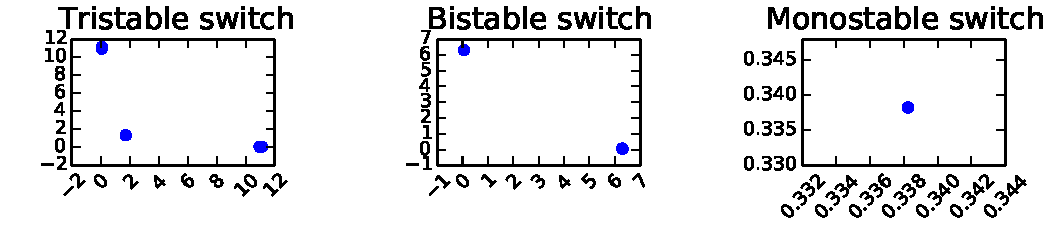
\includegraphics[scale=0.9]{../../chapters/chapterStabilityFinder/images/switch_stbility_examples.pdf}
%\captionof{figure}{An example for each type of switch found during the parameter scan. Each graph represents the steady state values of one dimer plotted against the other, from one parameter set and 100 initial conditions.}
%    \label{fig:stab exampl}
%\end{figure}
%
%In order to determine which areas in the parameter space give rise to the different kinds of stability, a histogram of the frequency of each parameter value found in monostable, bistable and tristable systems was plotted and shown in Figure~\ref{fig:scan ode param hist}.
%
%
%\begin{figure}
%\centering
%\begin{minipage}[c]{1\textwidth}
%\centering
%    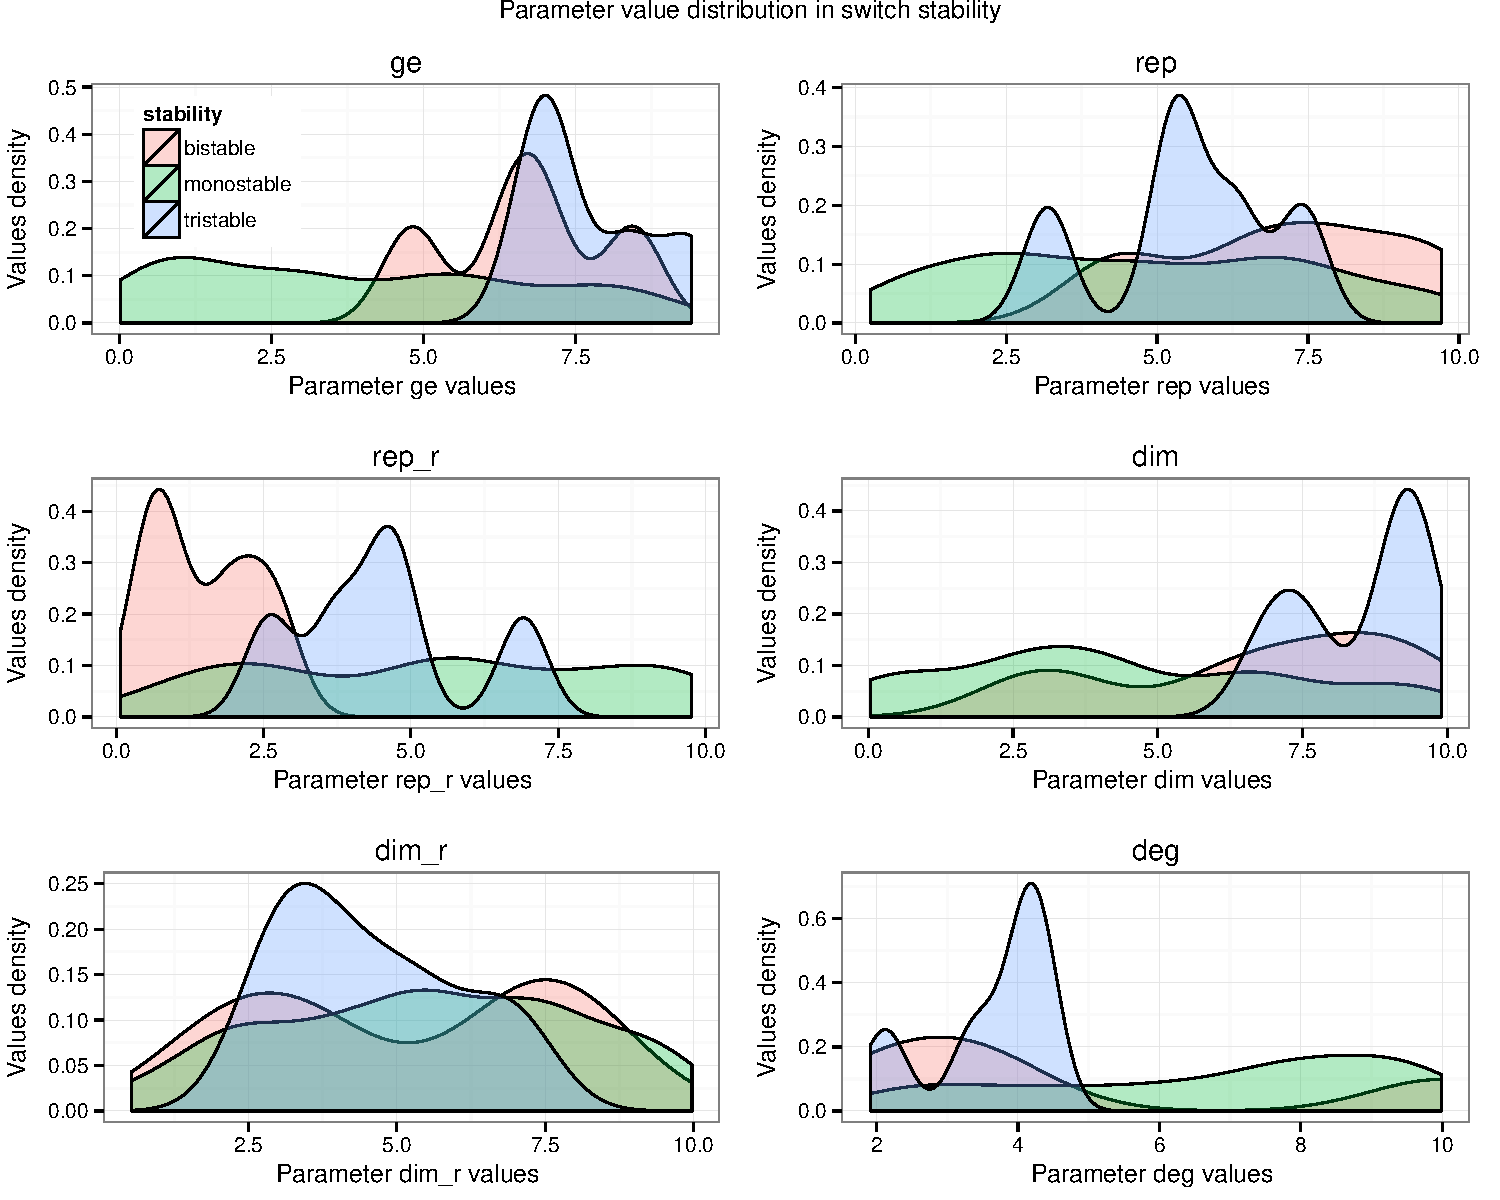
\includegraphics[width=1.05\textwidth]{../../chapters/chapterStabilityFinder/images/param_stability_hist.pdf}
%    \caption{The distribution of parameter values that resulted in monostable, bistable and tristable switches in the parameter scan. Each graph represents the distribution of the values of one parameter. }
%    \label{fig:scan ode param hist}
%\end{minipage}
%\end{figure}
%
%
%
%\begin{table}[h!]
%\centering
%\caption {The parameter values obtained from the parameter scan that resulted in bistability. Each row corresponds to a set of parameter values.} \label{tab: scan params}
%\begin{tabular}{ccccccc}
%\toprule
% \textbf{ge}     & \textbf{rep}    & \textbf{rep r}     & \textbf{dim}    & \textbf{dim r}     & \textbf{deg      }\\
% \midrule
%6.95   & 9.53    & 1.890     & 6.43   & 7.06      & 2.91   \\
%4.82   & 4.37    & 0.595     & 9.45   & 2.07      & 3.72   \\
%8.44   & 6.53    & 0.818     & 8.15   & 3.59      & 9.99   \\ 
%6.46   & 7.92    & 2.650     & 3.07   & 8.01      & 1.91   \\
%8.15   & 9.42    & 1.44      & 6.13   & 5.45      & 4.84     \\
%8.89   & 8.98    & 5.39      & 3.56   & 7.39      & 2.24     \\
%8.01   & 9.95    & 5.69      & 5.95   & 4.01      & 1.90     \\
%6.28   & 4.88    & 2.11      & 4.96   & 2.44      & 4.24     \\
%9.48   & 9.40    & 3.69      & 2.16   & 3.95      & 2.08     \\
%7.72   & 6.19    & 2.31      & 5.97   & 1.58      & 5.40     \\
%3.60   & 3.80    & 0.43      & 8.90   & 4.66      & 2.24     \\
%8.23   & 4.31    & 2.07      & 7.94   & 3.52      & 6.32     \\
%9.36   & 7.33    & 7.47      & 8.19   & 9.87      & 2.99   \\
%8.16   & 2.08    & 1.36      & 3.29   & 8.27      & 1.62   \\
%8.52   & 8.09    & 4.41      & 4.25   & 1.23      & 6.48   \\
%8.15   & 4.42    & 1.05      & 5.44   & 9.57      & 2.16   \\
%\bottomrule
%\end{tabular}
%\end{table}   
%   
%\clearpage
%\subsection{Discussion}
%\par
%   The parameter scan was successfully completed in the deterministic case and some of the results shown in Figure \ref{fig:stab exampl}. Different parameter sets resulted in different stability of the toggle switch.   
%     
%\par
%   There were a total of 217 monostable, 16 bistable and 6 tristable switches out of 400 sampled parameter sets. The remaining samples did not reach steady state. This shows that different parameter values have a great effect on the stability profile of the switch. Note the symmetry of the steady states of each bistable switch is due to the use of a symmetric model. 
% 
%\par 
%    Some interesting results arise from the histograms in Figure ~\ref{fig:scan ode param hist}. It can be seen that the parameter for gene expression (ge) tends to be relatively high when bistability arises whereas the parameter for the reverse reaction of repression (rep r) tends to be low. Degradation (deg) also tends to be low. It must also be noted that the parameter values that give rise to monostable systems are generally evenly distributed for all parameters, suggesting that monostable systems arise from the whole range of values sampled. This can further indicate that the right combination of more than one parameter values is necessary for bistability. Further analysis is thus needed to determine what these combinations are. A sensitivity analysis of the model will be carried out in order to determine which parameters affect bistability and to which parameters is the system robust. The parameter scan will also be incorporated into the ABC SMC methodology, in order to identify the parameter values required for bistability more efficiently.             
%
%\par
%    In this work it was shown that a range of stability profiles are achievable by the standard toggle switch. The patterns of the parameter values required for each are beginning to emerge. Further work is required in order to get a definitive answer for the stability characteristics of the toggle switch given this modelling approach.
%
%\section{Bayesian approach to model stability}
\section{StabilityFinder algorithm}

To investigate the multistable behaviour of systems, I had to make a number of extensions to existing approaches. Firstly, a wide range of initial condition samples are required in order to determine the stability of a system. For a given set of parameter values, sample points are taken across initial conditions using latin hypercube sampling~\autocite{MCKAY:2000vt}, and the ensemble system simulated in time until steady state. As a distance function I use the desired stability of the simulated model. An overview of the algorithm is given in Section~\ref{sec:Alg_overview}. %Then each module in the algorithm is described in Sections~\ref{sec:part_samp}-\ref{sec:mod_check}.


\subsection{Algorithm overview}
\label{sec:Alg_overview}
The StabilityFinder algorithm is summarised below. StabilityFinder is available as a Python package, and can be downloaded from \url{https://github.com/ucl-cssb/StabilityFinder.git}. 

\begin{figure*}[h]
\begin{center}
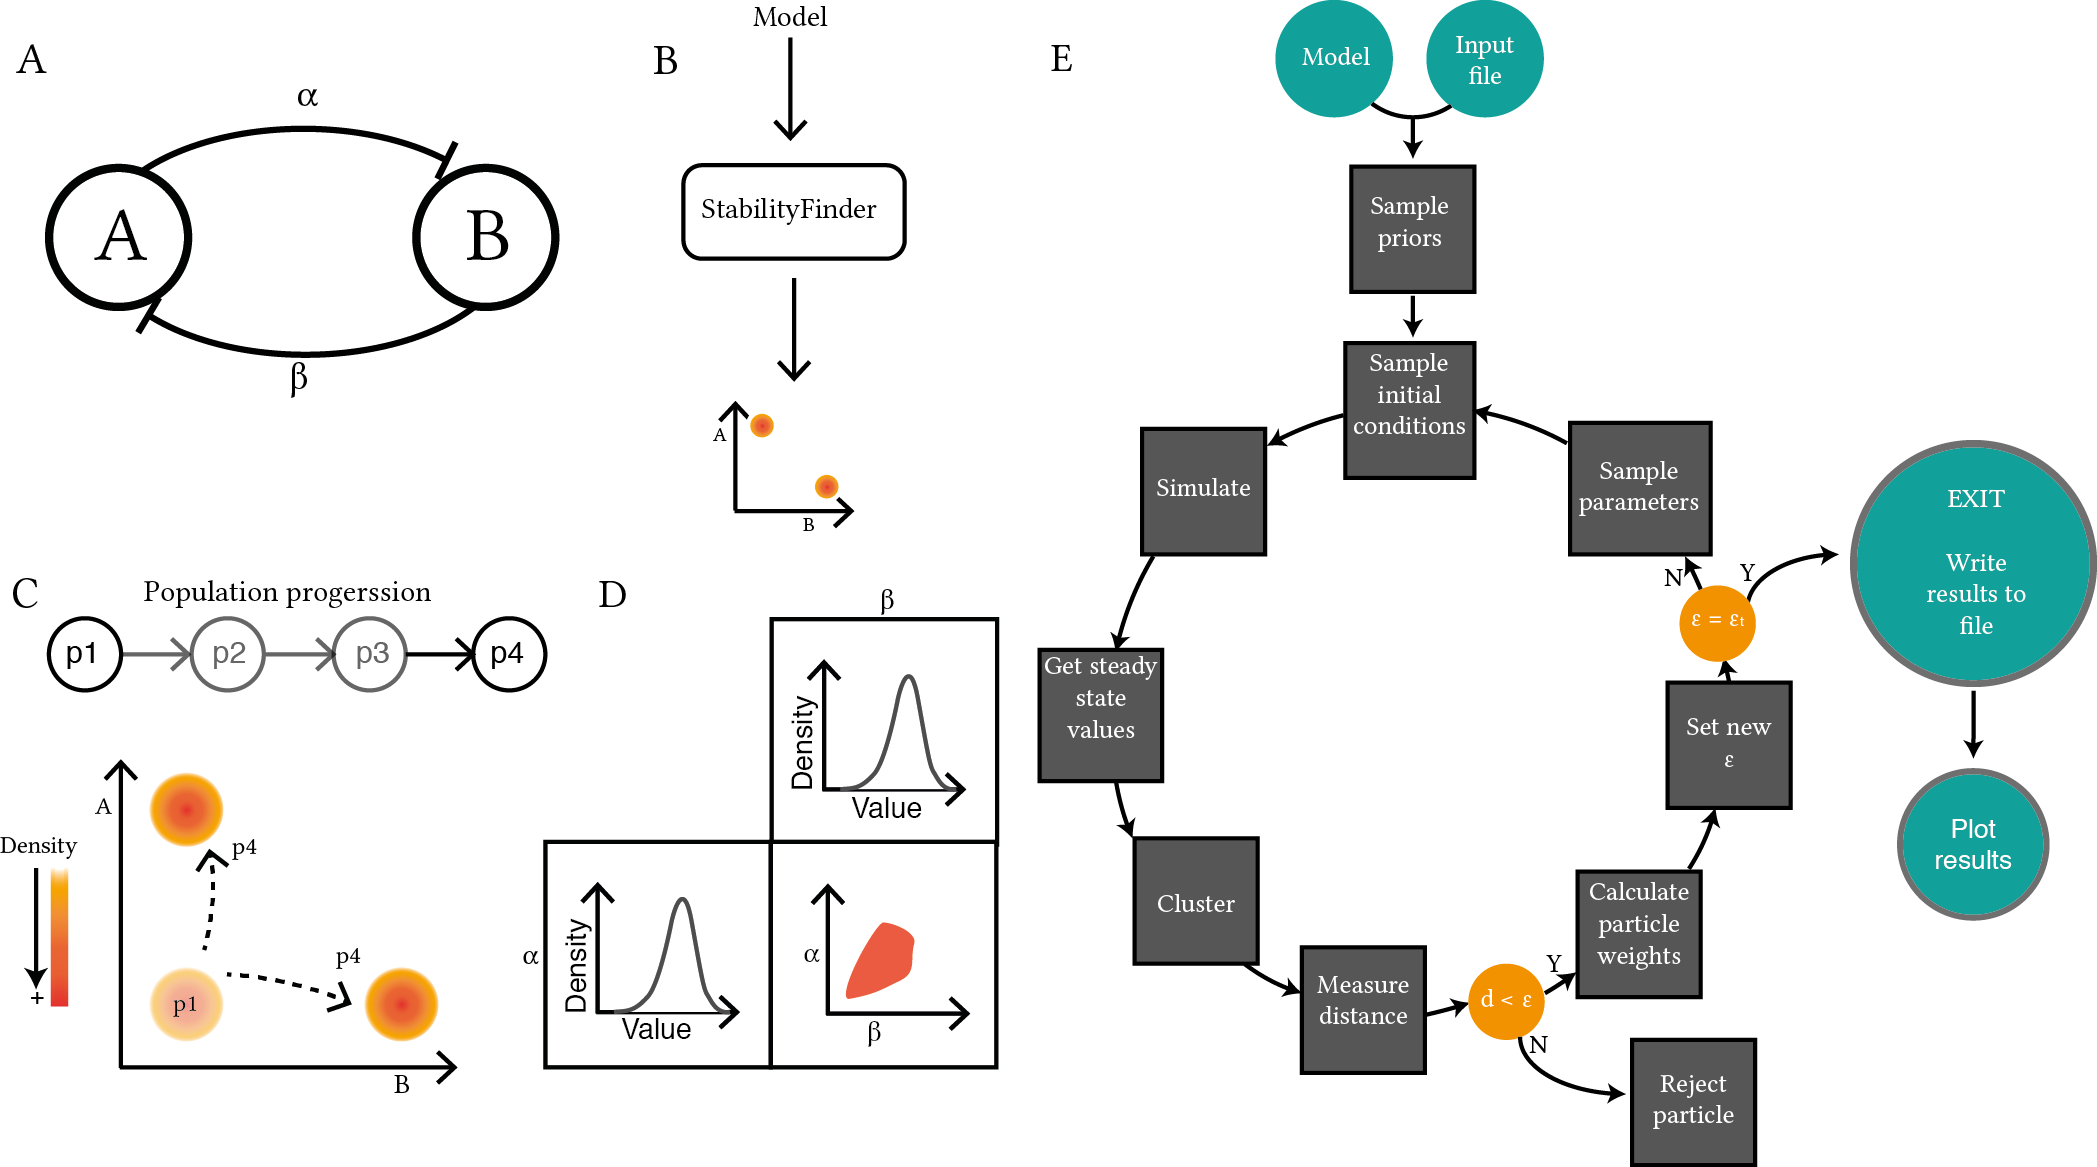
\includegraphics[scale=0.9]{../../chapters/chapterStabilityFinder/images/SF_algo_overv.png}
\caption[StabilityFinder algorithm overview]{\label{fig:fig1}: Using sequential Monte Carlo to examine system stability. The algorithm takes as input a model (A) and evolves it to the stability of choice (C) via intermediate populations. In this example model shown in A, There are two species and two parameters. For the model to be bistable, the phase plot of the two species of interest must have two distinct densities, as shown in (C). The parameter space of the model is searched through our algorithm until the resulting simulations give rise to bistability. The parameter values for the model that demonstrated the desired behaviour are given as an output (D). The output consists of the accepted values for each parameter, as well as each density plotted against the other. This allows us to uncover correlations between parameter values. We made this algorithm into a python package, called StabilityFinder. The overview of the algorithm is shown in (E).}
\end{center}
\end{figure*}
\clearpage

The user provides an SBML model file~\autocite{Finney:2003vk, Hucka:2004wh} and an input file that contains all the necessary information to run the algorithm, including the desired stability and the final tolerance, $\epsilon$, for the distance from the desired behaviour necessary for the algorithm to terminate. The flow of execution is illustrated in Figure~\ref{fig:fig1}E. Since the algorithm is computationally intensive, all deterministic and stochastic simulations are performed using algorithms implemented on \acrfull{gpu}s, which are used for mutli-threaded computation~\autocite{Kirk:2010we}.


%The user provides an SBML model file and an input file that contains all the necessary information to run the algorithm, including the desired stability and the final tolerance \textepsilon, for the distance from the desired behaviour necessary for the algorithm to terminate. The flow of execution is illustrated in Figure~\ref{fig:fig1}E. Since the algorithm is computationally intensive, all deterministic and stochastic simulations are parallelised and performed using algorithms implemented on \acrfull{gpu}s. 

%\begin{figure*}[h]
%\begin{center}
%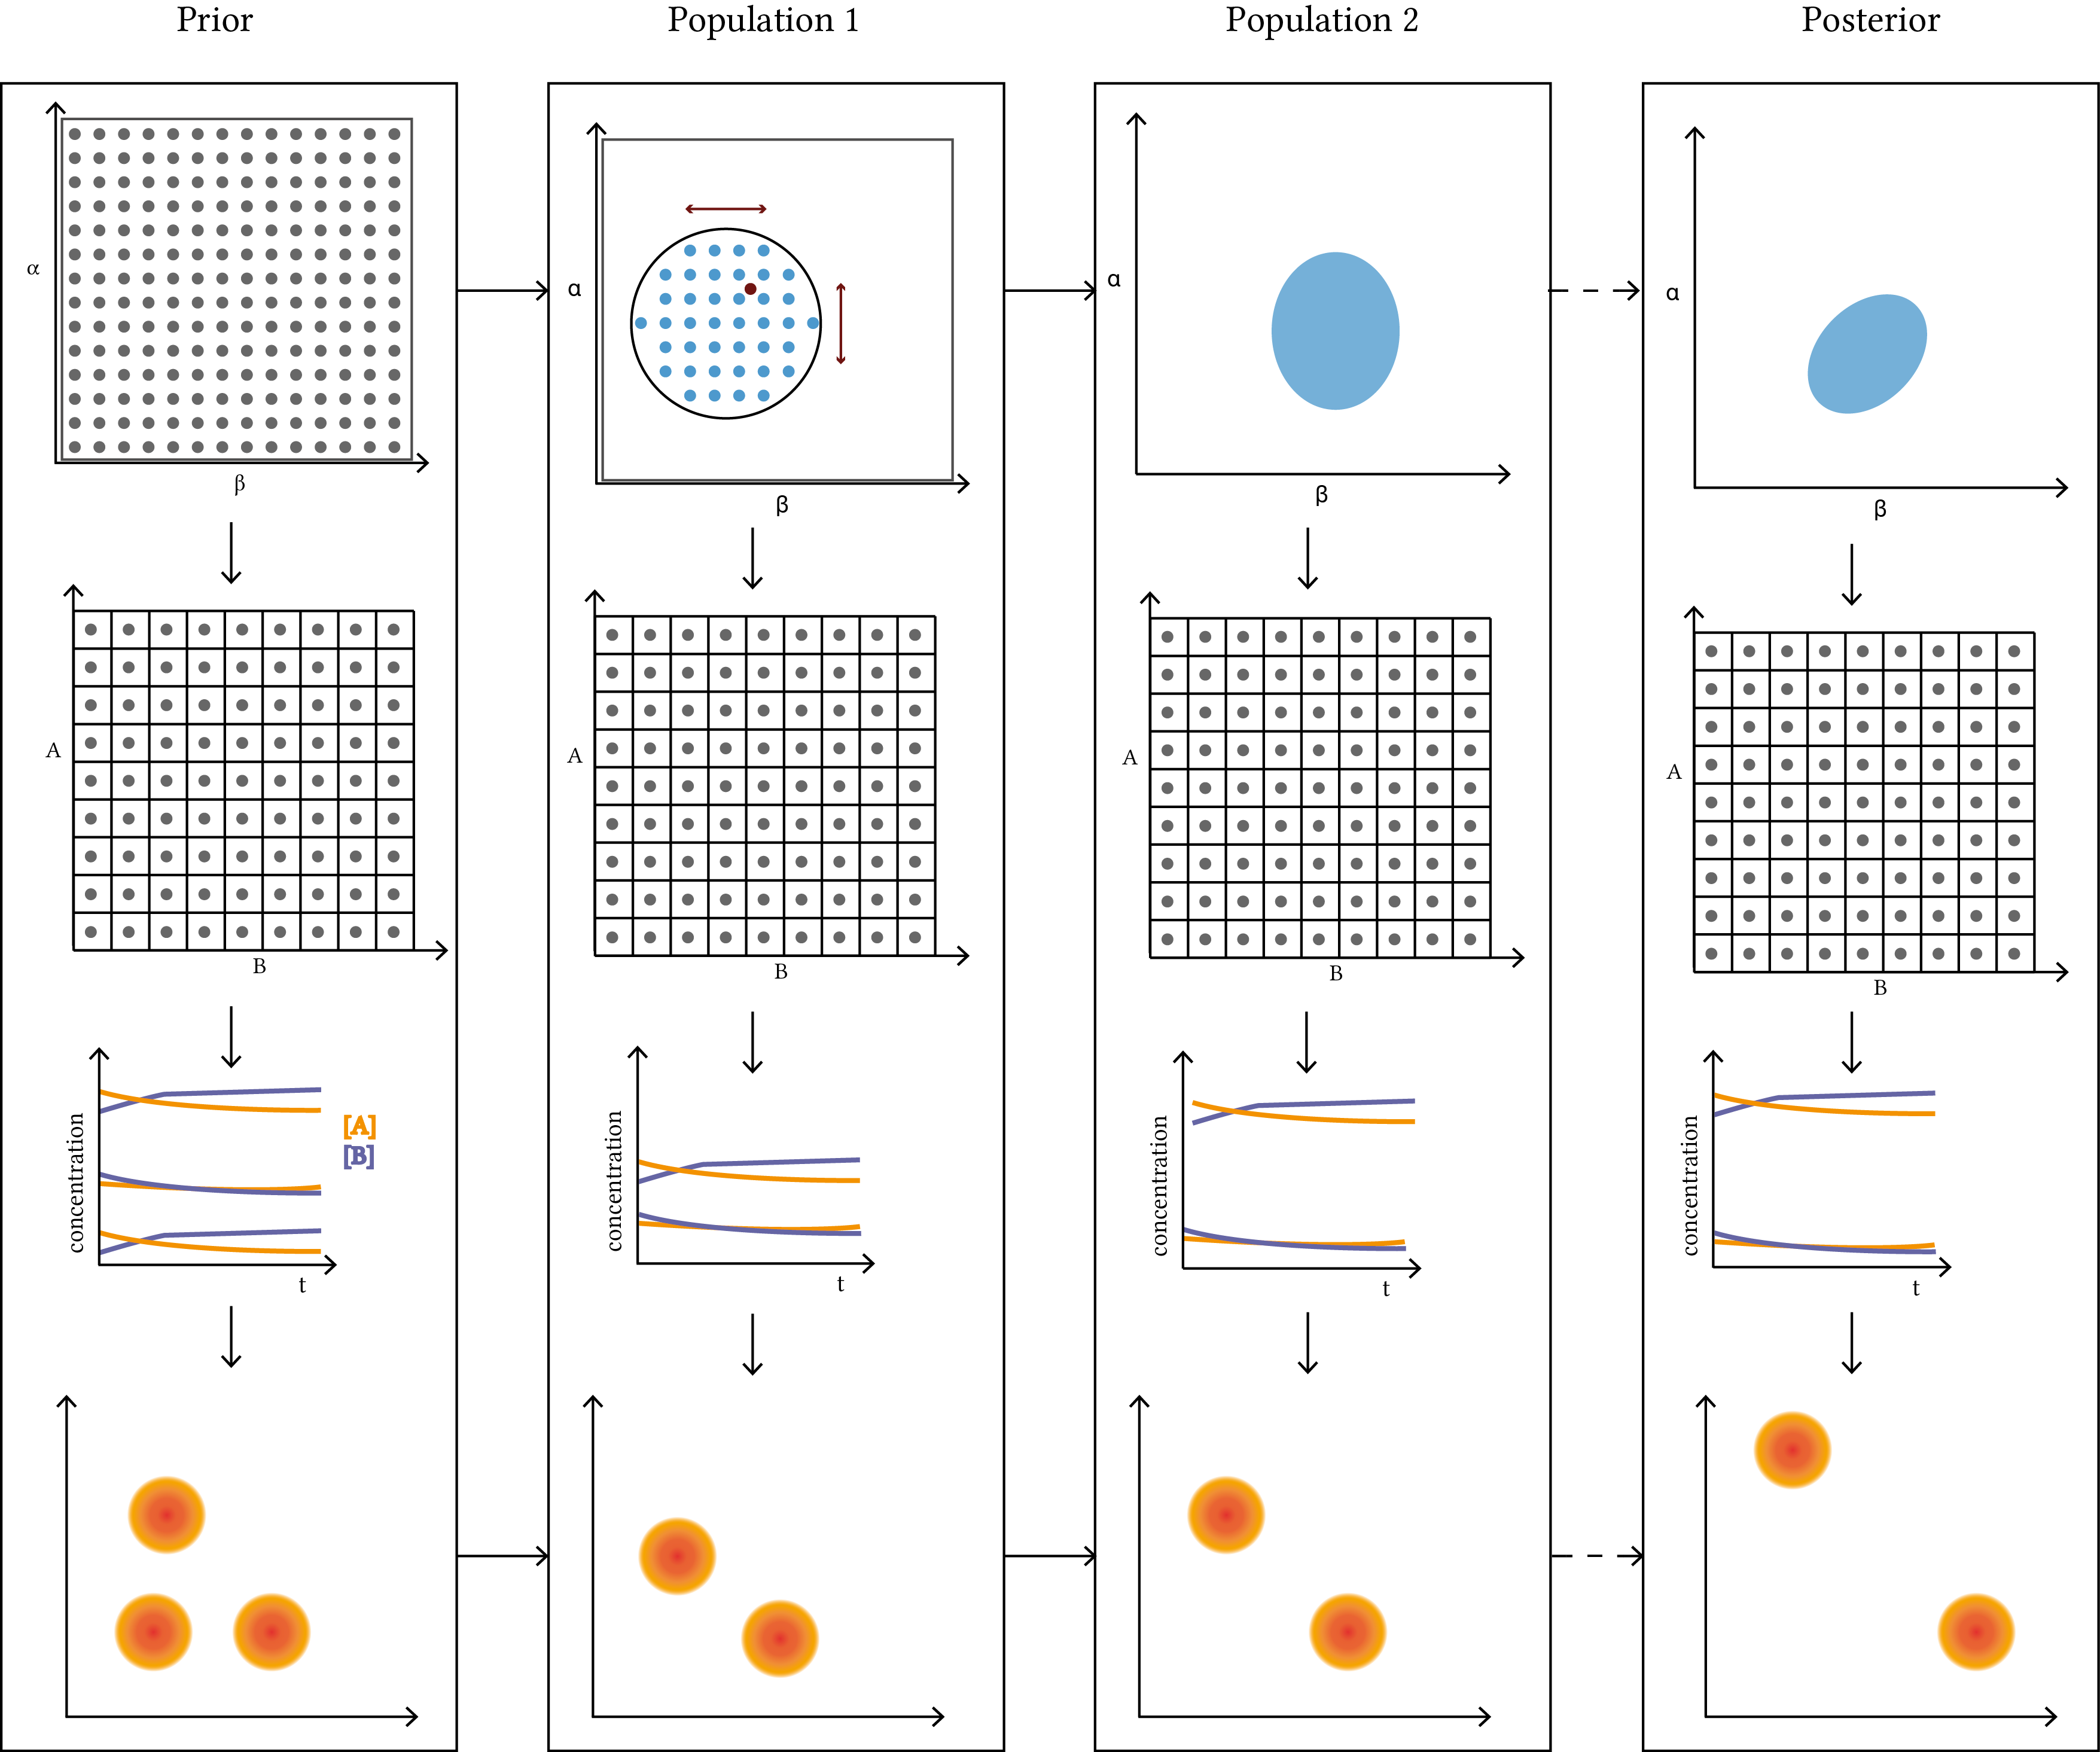
\includegraphics[scale=0.5]{../../chapters/chapterStabilityFinder/images/process_overv.png}
%\caption[LoF caption]{q}
%\end{center}
%\end{figure*}
%\clearpage

%\subsection{Particle sampling}
%\label{sec:part_samp}
%For the first population, particles are sampled from the priors. Random samples are taken from the distribution specified by the user for each parameter. 
%
%For subsequent populations particles are sampled from the previous population. The weight of each particle in the previous population dictates the probability of it being sampled. The number of samples to be drawn is specified by the user in the input file.  
%
%\subsection{Perturbation}
%\label{sec:pertub}
%Each sampled particle is perturbed by a kernel defined by the distribution of the previous population, as developed by~\textcite{Toni:2009tr}. 
%
%\begin{align}
%K_p(\theta|\theta* ) =& \theta* + U(+s_p, -s_p)\text{, where:} \\
%s_p =& \frac{1}{2} \big (max(\theta_{p-1}) - min(\theta_{p-1}) \big )
%\end{align}
%
%If the \texttheta* falls out of the limits of the priors then the perturbation is rejected and repeated until an acceptable \texttheta* is obtained. This method is successful in perturbing the particles by a small amount in order to explore the parameter space, but can be slow to complete. 

\subsection{Initial condition sampling}
\label{sec:init_cond_samp}
In StabilityFinder, latin hypercube sampling is used to sample initial conditions~\autocite{MCKAY:2000vt}. This is used to ensure that the whole space is sampled uniformly. Latin hypercube sampling is done in two dimensions in StabilityFinder. This is the same algorithm used for initial condition sampling in Chapter~\ref{ch:abcsysbio}, and the reader is referred to Section~\ref{sec:paramscan} for a description of this algorithm. StabilityFinder could easily be implemented to be used for a larger number of species, but here it has only been used for stability analyses concerning two species. Stability landscapes involving more that two species are beyond the scope of this thesis. %The uniform priors of the two species in consideration represent a rectangle space, which is subdivided into equal parts. Then a random sample is drawn from each sub-part. This ensures the whole space is evenly sampled. 

%\begin{figure*}[htbp]
%\begin{center}
%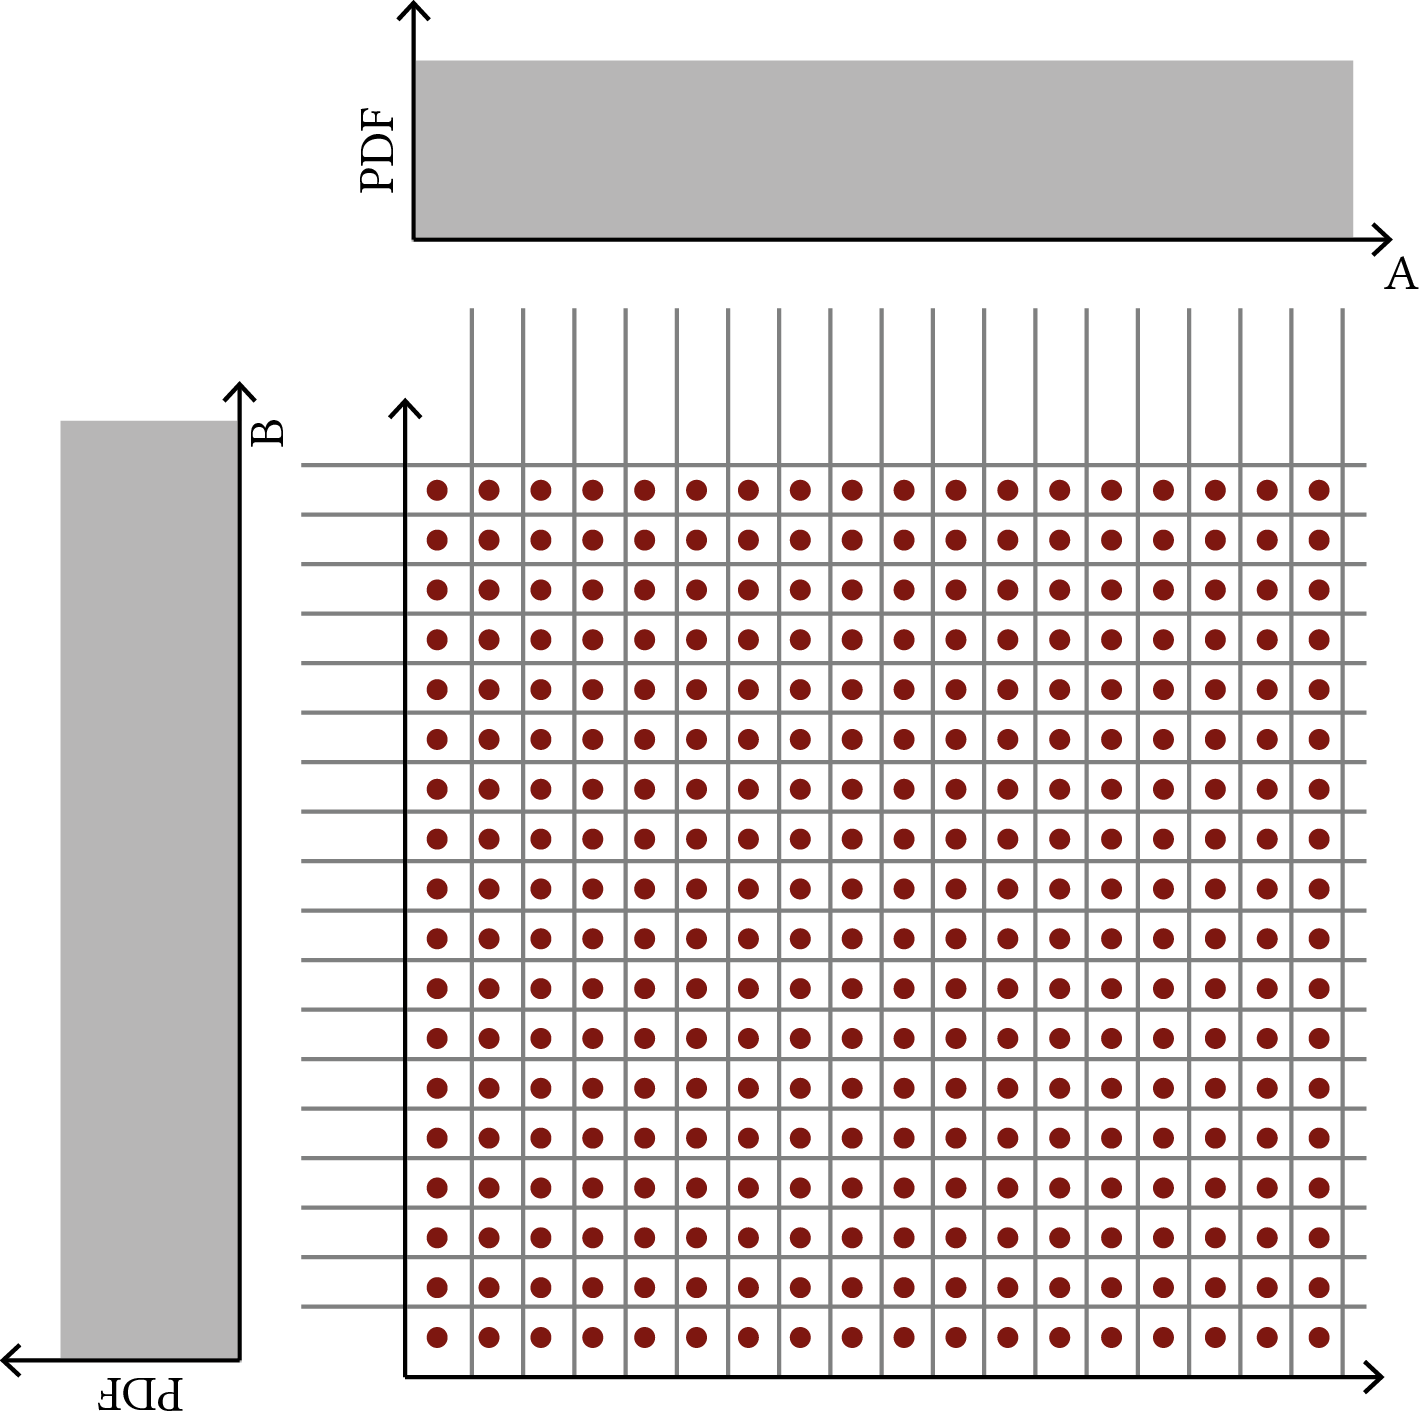
\includegraphics[scale=0.5]{../../chapters/chapterStabilityFinder/images/LHS.png}
%\caption[LoF caption]{\label{fig:lhs}Latin hypercube sampling ensures that the whole space is sampled evenly. For the two species concerned, A and B, we assume uniform distributions, shown in grey. The joint space of the two distributions is divided into smaller equal parts and a random sample is drawn from within each subspace.  }
%\end{center}
%\end{figure*}


\clearpage

%\subsection{Particle simulation}
%\label{sec:sim}
%Each particle is simulated using cuda-sim~\autocite{Zhou:2011hp}. The model is provided by the user in SBML format and is converted into CUDA\textsuperscript{\textregistered} code by cuda-sim. The model in CUDA\textsuperscript{\textregistered} code format can then be run on NVIDIA\textsuperscript{\textregistered}. CUDA\textsuperscript{\textregistered}. \acrshort{gpu}s. This allows the user to take advantage of the speed of parallelised simulations without any CUDA\textsuperscript{\textregistered} knowledge. 
%
 
\subsection{Clustering methods}
\label{Clustering methods}

Whether the model was simulated using \acrshort{ode}s or the Gillespie algorithm~\autocite{Gillespie:1977ww} dictated the method of clustering that I used. For the deterministic models I used an algorithm I developed, that will be referred to as the delta clustering algorithm in this thesis. This algorithm consists of defining the number of clusters by counting a new cluster every time a data point is more than a distance δ away from any existing clusters. The benefits of the delta clustering algorithm are that it is fast and can be used on deterministic solutions, where steady state values tend to be identical if all the particles have reached steady state.

Steady states of stochastic models are clustered using the K-means clustering~\autocite{Lloyd:1982wn} and the number of clusters determined using the Gap statistic~\autocite{Tibshirani:2001vo}. This method is more suited to stochastic solutions, where the delta clustering method would fail as the steady state solutions tend to be more widely dispersed than in the deterministic case. The detailed algorithms used are shown in Appendix~\ref{ap:Alg}. 

The method used for clustering can be altered by the user if he/she wants to add their own preferred clustering algorithm that might be more appropriate for their specific purposes. For the models I used here, the above methods were successful in clustering the steady state solutions. 

\subsection{Distance function}
\label{sec:dist}
 The distance function is used to compare the desired behaviour to the behaviour observed in each particle~\autocite{Toni:2009tr}. In StabilityFinder the distance function consists of three distances. The first one is the difference between the number of desired clusters and the number of clusters observed in the phase plot. For this distance metric the number of clusters in the phase plot must be calculated. The clustering methods used are outlined in Section~\ref{Clustering methods}.
 
 The other two distance metrics used in StabilityFinder are the variance within each cluster and the overall, between cluster, variance. The within cluster variance ensures that the clusters are tight, and the between cluster variance is used to ensure the clusters are far apart from each other. In the context of this thesis, the ideal behaviour of a system is tight, widely separated clusters. This means that the genetic system has distinct steady states, and the difference in the protein levels between each steady state is observable.

\begin{align}
	d_1 &= C = M_c \label{eq:dist1}\\
	d_2 &= V_{tot} = \frac{1}{n} \sum_{i=1}^{n}(x_i- \mu)	\label{eq:dist1}\\
	d_3 &= V_{cl} =  \underset{m_c = 1}{\overset{Mc}{\mathrm{median}}} \{ \frac{1}{n_{m_c}} \sum_{c=1}^{n_{m_c}}(x_c- \mu_c)\} \label{eq:dist3},
\end{align}
where $n$ denotes the total number simulations per particle, $x$ refers to each  simulation steady state of a given particle and μ the mean value of all the simulations steady states in each particle. $M_c$ denotes the total number of clusters per particle and $m_c$ refers to each cluster. $x_c$ and $\mu_c$ represent the simulation steady state of a given particle in the current cluster and the mean of the current cluster respectively.   


%\subsection{Particle rejection}
%\label{sec:rej}

Once the distance from the desired behaviour has been calculated, the algorithm rejects any particles whose distance is farther than the current ε. The distances taken into account are the number of clusters (C), the total variance (V\textsubscript{tot}) and the within cluster variance (V\textsubscript{cl}) as outlined in Equations~\ref{eq:dist1}-\ref{eq:dist3}. In addition to these distances I have included another two checks for the particles. Firstly, StabilityFinder checks if the simulation of a particle has reached steady state. If the standard deviation of the last ten time points in the simulation (denoted as $SS_{ss}$) is larger than a user-specified value, then the particle is rejected. This is to ensure that only particles that have reached steady state are considered. Secondly, there is a check for the minimum level of the steady states (denoted as $SS_{l}$). This is to allow the user to select for steady states whose protein levels are above a certain threshold. This has to be added as an additional check as the steady state levels must be experimentally observable if they are to be used to design new systems. Two steady state levels of very low levels would be biologically indistinguishable and thus meaningless in an experimental setup. This check is optional to the user, and can be set to zero if not desired. In summary, a particle must satisfy all of the criteria given below in order to be accepted:

\begin{align*}
	M_c &\leq ε_{M_c} \\
	V_{tot} &\leq ε_{V_{tot}}\\
	V_{cl} &\leq ε_{V_{cl}}\\
	SS_{ss} &\leq ε_{SS_{ss}}\\
	SS_{l} &\leq ε_{SS_{l}}
\end{align*}



%\begin{enumerate}
%	\item Cluster distance \textgreater \textepsilon\textsubscript{c}
%	\item V\textsubscript{bc} distance \textgreater \textepsilon \textsubscript{Vbc}
%	\item V\textsubscript{wc} distance \textgreater \textepsilon \textsubscript{Vwc}
%	\item SS\textsubscript{v} \textgreater \textepsilon \textsubscript{ssv}
%	\item SS\textsubscript{l}  \textgreater \textepsilon \textsubscript{ssl}
%\end{enumerate}
% 

%\subsection{Weight calculation}
%\label{sec:weight}
%For the first population the weights are all given a value of 1, and then normalised over the number of particles. For subsequent populations the weights of the particles are calculated by considering the weights of the previous population~\autocite{Toni:2009tr}. 
%
%\begin{align}
%w_{t}^{(i)} = \frac{P(\theta_{t}^{(i)})}{\sum_{j=1}^N w_{t-1}^{(j)} K_{t}(\theta_{t-1}^{(j)}, \theta_{t}^{(i)})} \text{ for n $\textgreater$  0}
%\end{align}
%	
%The weights are then normalised over the total number of particles. 
%    

\subsection{Model checking}
\label{sec:mod_check}
A problem that can arise by using this method with stochastic simulations is that the behaviour observed may not be the true behaviour but it might be a result of noise. We need to ensure that the resulting behaviour is reproducible. Therefore, I added model checking to the algorithm. Model checking consists of resampling from the posterior distribution and simulating each sample. If the resulting behaviour is the same as what we expected we can be confident that it is the true behaviour of the system and not a result of noise. 
\begin{algorithm}[htbp]

\caption{ StabilityFinder algorithm}
\label{alg:StabilityFinder}
 \begin{algorithmic}[1]
    \Statex
	\State Initialise $t=0$, 
	\State $i=0$ 
	\If{t $= 0$}
		\State Sample particle from prior, $\theta^{**} \sim \pi(\theta)$
	\Else
		\State Sample $\theta^*$ from the previous population $\{ \theta_{t-1}^{i} \}$ with weights $w_{t-1}$.
		\State Perturb the particle, $\theta^{**} \sim K_t(\theta|\theta^{*})$ where $K_t$ is the perturbation kernel.
	\EndIf
	
	\State Sample $k$ initial conditions $\{ x_0^k \}$ via latin hypercube sampling.
	\State Simulate $k$ datasets to steady state, $\{ x^{*k} \}$, from the the model, $ x^{*} \sim f(x|\theta, x_0)$
    	\State Apply clustering in phase space on $\{ x^{*k} \}$
    	\State Calculate the distance $ d = \rho( \{ x^{*k} \},y)$. 
    	\If{$d \leq \epsilon_t$}
	\State $\theta^{i}_{t} = \theta^{**}$.  $i = i + 1$
	\If{ $i \le N$ } 
		GoTo step 3
	\Else
	\State Calculate weight for each accepted $\theta^{i}_t$
	\State $w_{t}^{(i)} = \begin{cases} 1, & \mbox{if } t = 1 \\\frac{\pi(\theta_{t}^{(i)})}{\sum_{j=1}^N w_{t-1}^{(j)} K_{t}(\theta_{t-1}^{(j)}, \theta_{t}^{(i)})}, & \mbox{if } p \geq  1. \end{cases}$
	\State Normalise weights
	\State $t = t + 1$. 
	\If{ $t \le N_t$} 
	\State GoTo step 3 
	\EndIf
	\EndIf
	\EndIf	
\end{algorithmic} 
\end{algorithm}

\clearpage

\section{Calculating robustness}
\label{sec:cal_rob}
Unlike~\textcite{Toni:2009tr}, StabilityFinder does not have model selection integrated into the method. This is because the purpose of StabilityFinder is not necessarily to compare models for robustness but to elucidate the stability a given model is capable of. Nevertheless, robustness analysis is an outcome that Bayesian methods are well suited for. Therefore, here I discuss another algorithm I developed in order to extract robustness information from the results of StabilityFinder and apply model selection.  

As discussed in Section~\ref{sec:rob_back}, two models $M_a$ and $M_b$ can be compared for their robustness using the Bayes factor, defined as follows:

\begin{align}
 B_{ab} &= \frac{p(D|M_a)}{p(D|M_b)}, \label{eq:final_bayes1}
\end{align}	

\noindent which represents the fraction of the evidence supported by model $a$ over the evidence supported by model $b$. This can be interpreted as the ratio of the fraction of the volume of the functional region to the volume of its prior of model $a$ and model $b$:

\begin{align}
 B_{ab} &= \frac{|F_a|}{|P_a|} / \frac{|F_b|}{|P_b|}, \label{eq:final_bayes2}
\end{align}	

\noindent where $|F|$ is the volume of the functional region of model and $|P|$ the volume of the prior. Equation~\ref{eq:final_bayes2} represents the ratio of the robustness measure of each model which in turn is defined as the ratio between the volume of functional region $F$ and the volume of the prior $P$. The reader is referred to Section~\ref{sec:rob_back} for a further discussion.

In order to calculate the Bayes factor we must first be able to approximate the volume of the viable parameter space. The viable parameter space is the space that approximates the posterior distribution that can give rise to the desired behaviour. I tested two methods of approximating the volume of the viable space, which are outlined in Algorithm~\ref{alg:robustness}. The first method is based on the method used by~\autocite{Hafner:2009ct}, where the volume of the cuboid containing all the viable space is calculated. I modified this part of their method by only including the area of the viable space where the majority of the last population lies. Therefore only the 1\textsuperscript{st} and 99\textsuperscript{th} percentile of the viable space are taken into account. This is necessary in order to exclude outliers in the distribution that would skew the volume calculation significantly. Each parameter represents a side in the cuboid and since the volume of a cuboid is equal to the product of its sides, the volume of the viable space is equal to the product of the ranges of all the parameters. This cuboid method will be prone to overestimating robustness especially in cases of correlation between parameters. This caveat could be alleviated if a \acrfull{pca}~\autocite{Fukunaga:2013wt} is done on the data before the cuboid is calculated~\autocite{Hafner:2009ct}. This would align the axes of the cuboid to the major axes of the distribution. This would still be a crude estimation of the volume, since if the posterior distribution is assumed to be normally distributed the volume would still be overestimated. 

Thus I used a second method, where the volume of the viable space was represented by a hyper-ellipsoid, an ellipse in higher dimensions. This method should not be as prone to overestimation of robustness as the cuboid method as an ellipsoid can take correlation into account. For this method the distribution of the viable space is assumed to be normal. The method calculates the covariance matrix of the distribution, whose volume is given by Equation~\ref{eq:el_vol}. Just as in the cuboid method, the 1\textsuperscript{st} and 99\textsuperscript{th} percentile of the data is ignored. 

\begin{align}
	V & = \frac{2\pi^{\frac{k}{2}}}{k\Gamma(\frac{k}{2})} \Big[ \chi _{k}^{2}(\alpha) \Big]^{\frac{k}{2}} |\Sigma|^\frac{1}{2}, \label{eq:el_vol}
\end{align}
\noindent where k is the number of dimensions, \textGamma{} is the Gamma function, \textalpha{} is the confidence interval required and |$\Sigma$| is the determinant of the covariance matrix. %In this case p = 3, \textalpha{} = 0.025

To validate these methods I compare them to ABC-SysBio model selection~\autocite{Liepe:2014iw}. ABC-SysBio has been used extensively for model selection~\autocite{Toni:2009tr, Toni:2011jy, Barnes:2011hh} and is thus used as a benchmark to the algorithm used here. We use two examples used in  the ABC-SysBio package~\autocite{Toni:2009tr} as well as in~\textcite{Toni:2010}. 
%There is good agreement between the three methods as can be seen in Figures~\ref{fig:rob_sysbio1} and \ref{fig:rob_sysbio4}.


\begin{algorithm}[htbp]
\caption{Approximating robustness}
\label{alg:robustness}

 \begin{algorithmic}[1]
 	\Let{k}{number of parameters}
 	\Let{i}{prior for each parameter}
    \Statex
		\For{each model $m$ of $M$}
		\State Prior$\sim U(a, b)$
    	\State $V_{prior}^{m} = \prod_{i=1}^{k} (i_{b} - i_{a})$ \
		\Statex
			\State Get $1^{st} < data < 99^{th}$ percentiles
    		\If{Cuboid calculation}
    		\State $V_{post}^{m} = \prod_{i=1}^{k} (i_{max} - i_{min})$ \
    		\EndIf
			\If{Ellipsoid calculation}
				\State Calculate data covariance matrix
    			\State $V_{post}^{m} = \frac{2\pi^{\frac{k}{2}}}{k\Gamma(\frac{k}{2})} \Big[ \chi _{k}^{2}(\alpha) \Big]^{\frac{k}{2}} |\Sigma|^\frac{1}{2}$
    		\EndIf
			\Statex
			\State $R^{m} = \frac{V_{post}^{m}}{V_{prior}^{m}}$
			
			\State $R_{norm}^{m} = \frac{R^{m}_i}{\sum_{i=1}^{M} R^m_i }$
		\EndFor
  \end{algorithmic}
\end{algorithm}	

\clearpage
\subsection{Case study 1: Infectious diseases}
\label{sec:cs1}

As described in~\textcite{Toni:2009tr}, the models used for the first case study describe the spread of an infectious disease through a population over time. The population is made up of susceptible, infected or recovered individuals, denoted as $S$, $I$ and $R$ respectively. Three models are compared for the robustness of their posterior distributions. The first model (Model 1), is the simplest model of the three. Each individual $S$ or $R$ can be infected once and then it can immediately infect other individuals~\autocite{Toni:2009tr}.

Model 1:
\begin{align*}
\frac{dS}{dt} &= \alpha - \gamma SI - dS \\
\frac{dI}{dt} &= \gamma SI - \upsilon I - dI \\
\frac{dR}{dt} &= \upsilon I - dR,
\end{align*}

\noindent where $a$ denotes the birth rate, $d$ the death rate, \textgamma{} the infection rate, and $v$ the recovery rate. The second model, Model 2, includes a time delay between an individual getting infected and being infectious. \textdelta{} denotes the rate of transition of a non-infectious infected individual to an infectious one.

Model 2:
\begin{align*}
\frac{dS}{dt} &= \alpha - \gamma SI - dS \\
\frac{dL}{dt} &= \gamma SI - \delta L - dL \\
\frac{dI}{dt} &= \delta L - \upsilon I - dI \\
\frac{dR}{dt} &= \upsilon I - dR,
\end{align*}

\noindent Finally the third model, Model 3, extends Model 1 and includes the recovered individuals being able to become susceptible again. This is denoted by rate $e$.

Model 3:
\begin{align*}
\frac{dS}{dt} &= \alpha - \gamma SI - dS + eR\\
\frac{dI}{dt} &= \gamma SI - \upsilon I - dI \\
\frac{dR}{dt} &= \upsilon I - dR - eR,
\end{align*}

\noindent The three models are simulated using \acrshort{ode}s. In ABC-SysBio model selection is used. Parameter inference is also used for each model separately without the use of model selection. I used the two methods outlined in Algorithm~\ref{alg:robustness} to calculate the robustness of the posterior distributions of all three models resulting from the parameter inference. This robustness measure was then compared to the result of ABC-SysBio model selection of the same models. As shown in Figure~\ref{fig:rob_sysbio1}, there is good agreement between the three measures of robustness. The posterior distributions of all three models are also shown in Figure~\ref{fig:rob_sysbio1}.

\subsection{Case study 2: Population growth}
\label{sec:cs2}
The second example I will use to demonstrate the effectiveness of the methods used here for robustness calculation is a population growth model. This is example is also used in the ABC-SysBio package~\autocite{Toni:2009tr}.

The data was obtained by simulating an immigration-death model shown in Equation~\ref{eq:id}. This model (referred to as Model 1) and a model of logistic growth are compared for robustness of their posterior distributions.
 
Model 1:
\begin{align}
  \frac{dI}{dt} &= \alpha - \beta I \label{eq:id}
\end{align}

\noindent Logistic growth, Model 2:

\begin{align}
  \frac{dI}{dt} &= \gamma - I	(\delta - \epsilon I)
\end{align}

%5{\color{red} check these equations}

\noindent As in Section~\ref{sec:cs1}, two analyses were carried out on these two models. First, ABC-SysBio model selection was used to find the most robust model. Then parameter inference was done on each model. The resulting posterior distributions (shown in Figure~\ref{fig:rob_sysbio4}), were compared for robustness using the cuboid and the ellipsoid approximation methods. All three robustness measures find that Model 1 is the most robust model. The analysis was repeated for~\acrshort{ode},~\acrfull{mjp} and~\acrfull{sde} simulations, all arriving to the same result of Model 1 being the most robust. The results are shown in Figure~\ref{fig:rob_sysbio4}.


\begin{figure*}[p]
\begin{center}
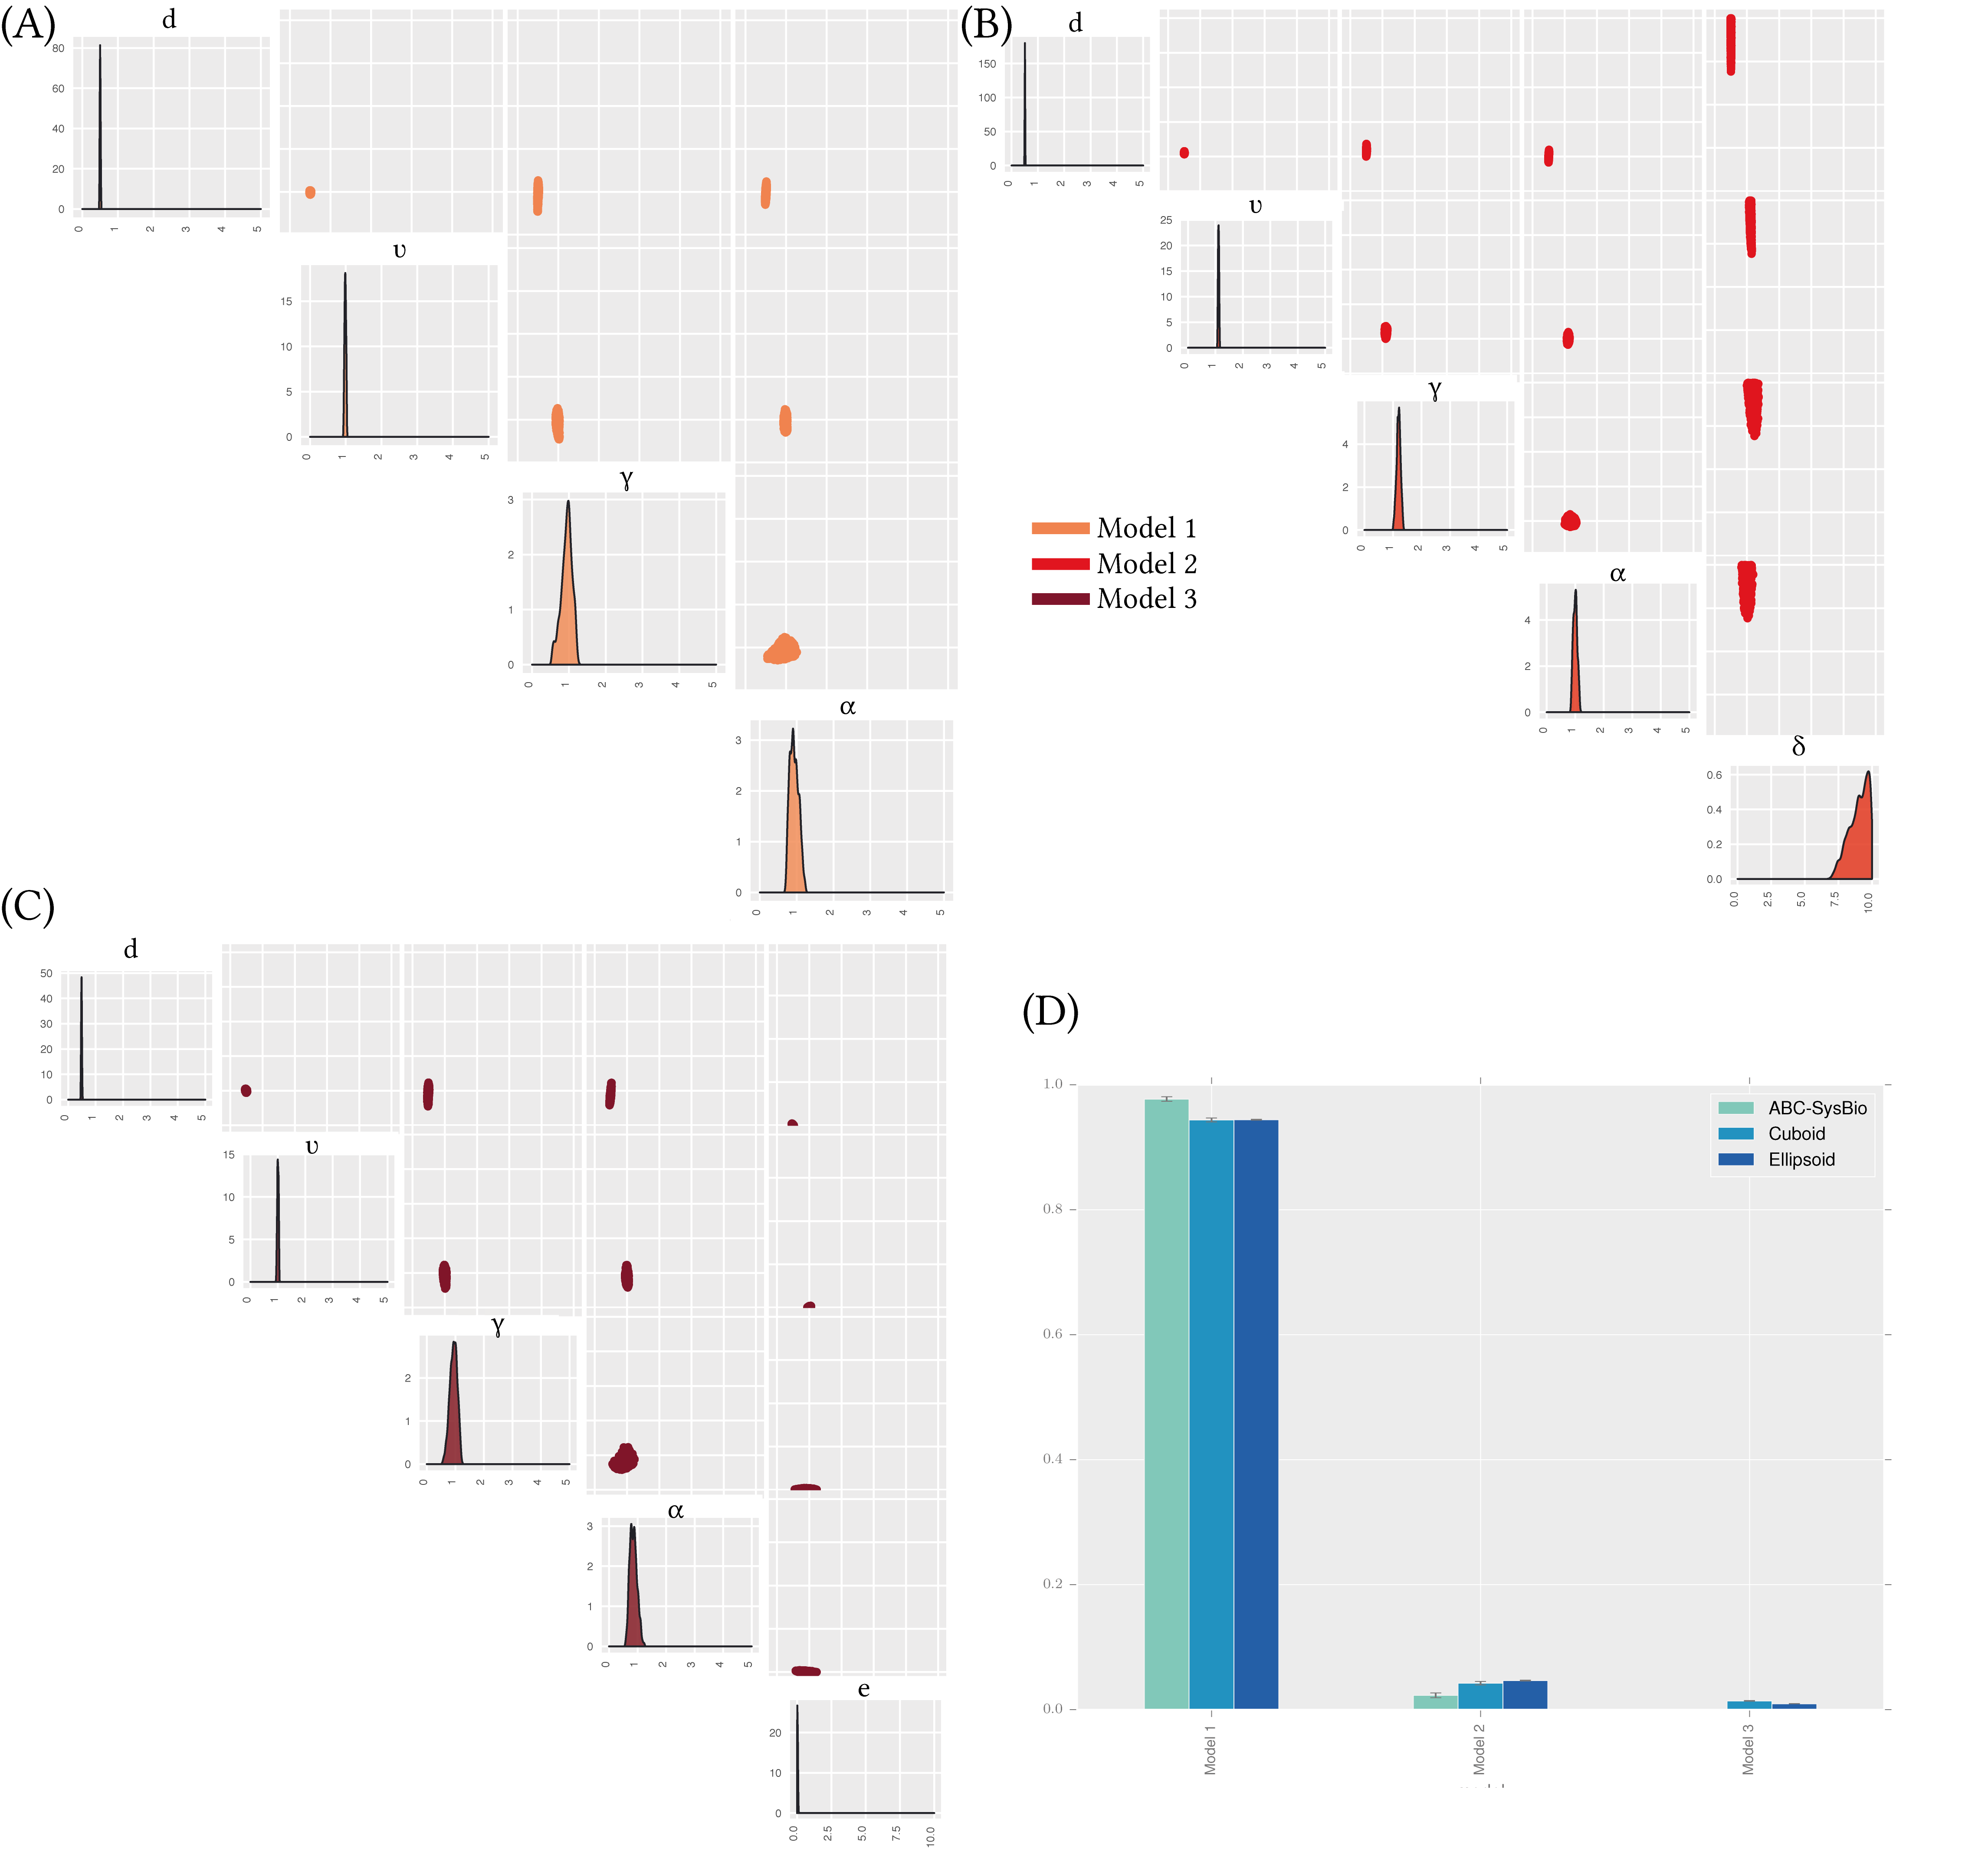
\includegraphics[width=\textwidth]{../../chapters/chapterStabilityFinder/images/ex1_sum.png}
\caption[Robustness analysis of case study 1]{\label{fig:rob_sysbio1}: Robustness analysis of the three models for the spread of infectious diseases. (A-C) The posterior distributions of the three models compared. (D) I use three methods to calculate robustness, ABC-SysBio model selection, the volume of the hyper-cuboid approximation of the posterior distribution and the volume of the hyper-ellipsoid approximation of the posterior distribution. Each analysis was repeated three times. The height of the bars indicate the mean robustness from the three repeats and the error bars represent the standard deviation. There is good agreement between all three methods. All three methods show that Model 1, the simplest model, is the most robust model. }

\end{center}
\end{figure*}

\begin{figure*}[p]
\begin{center}
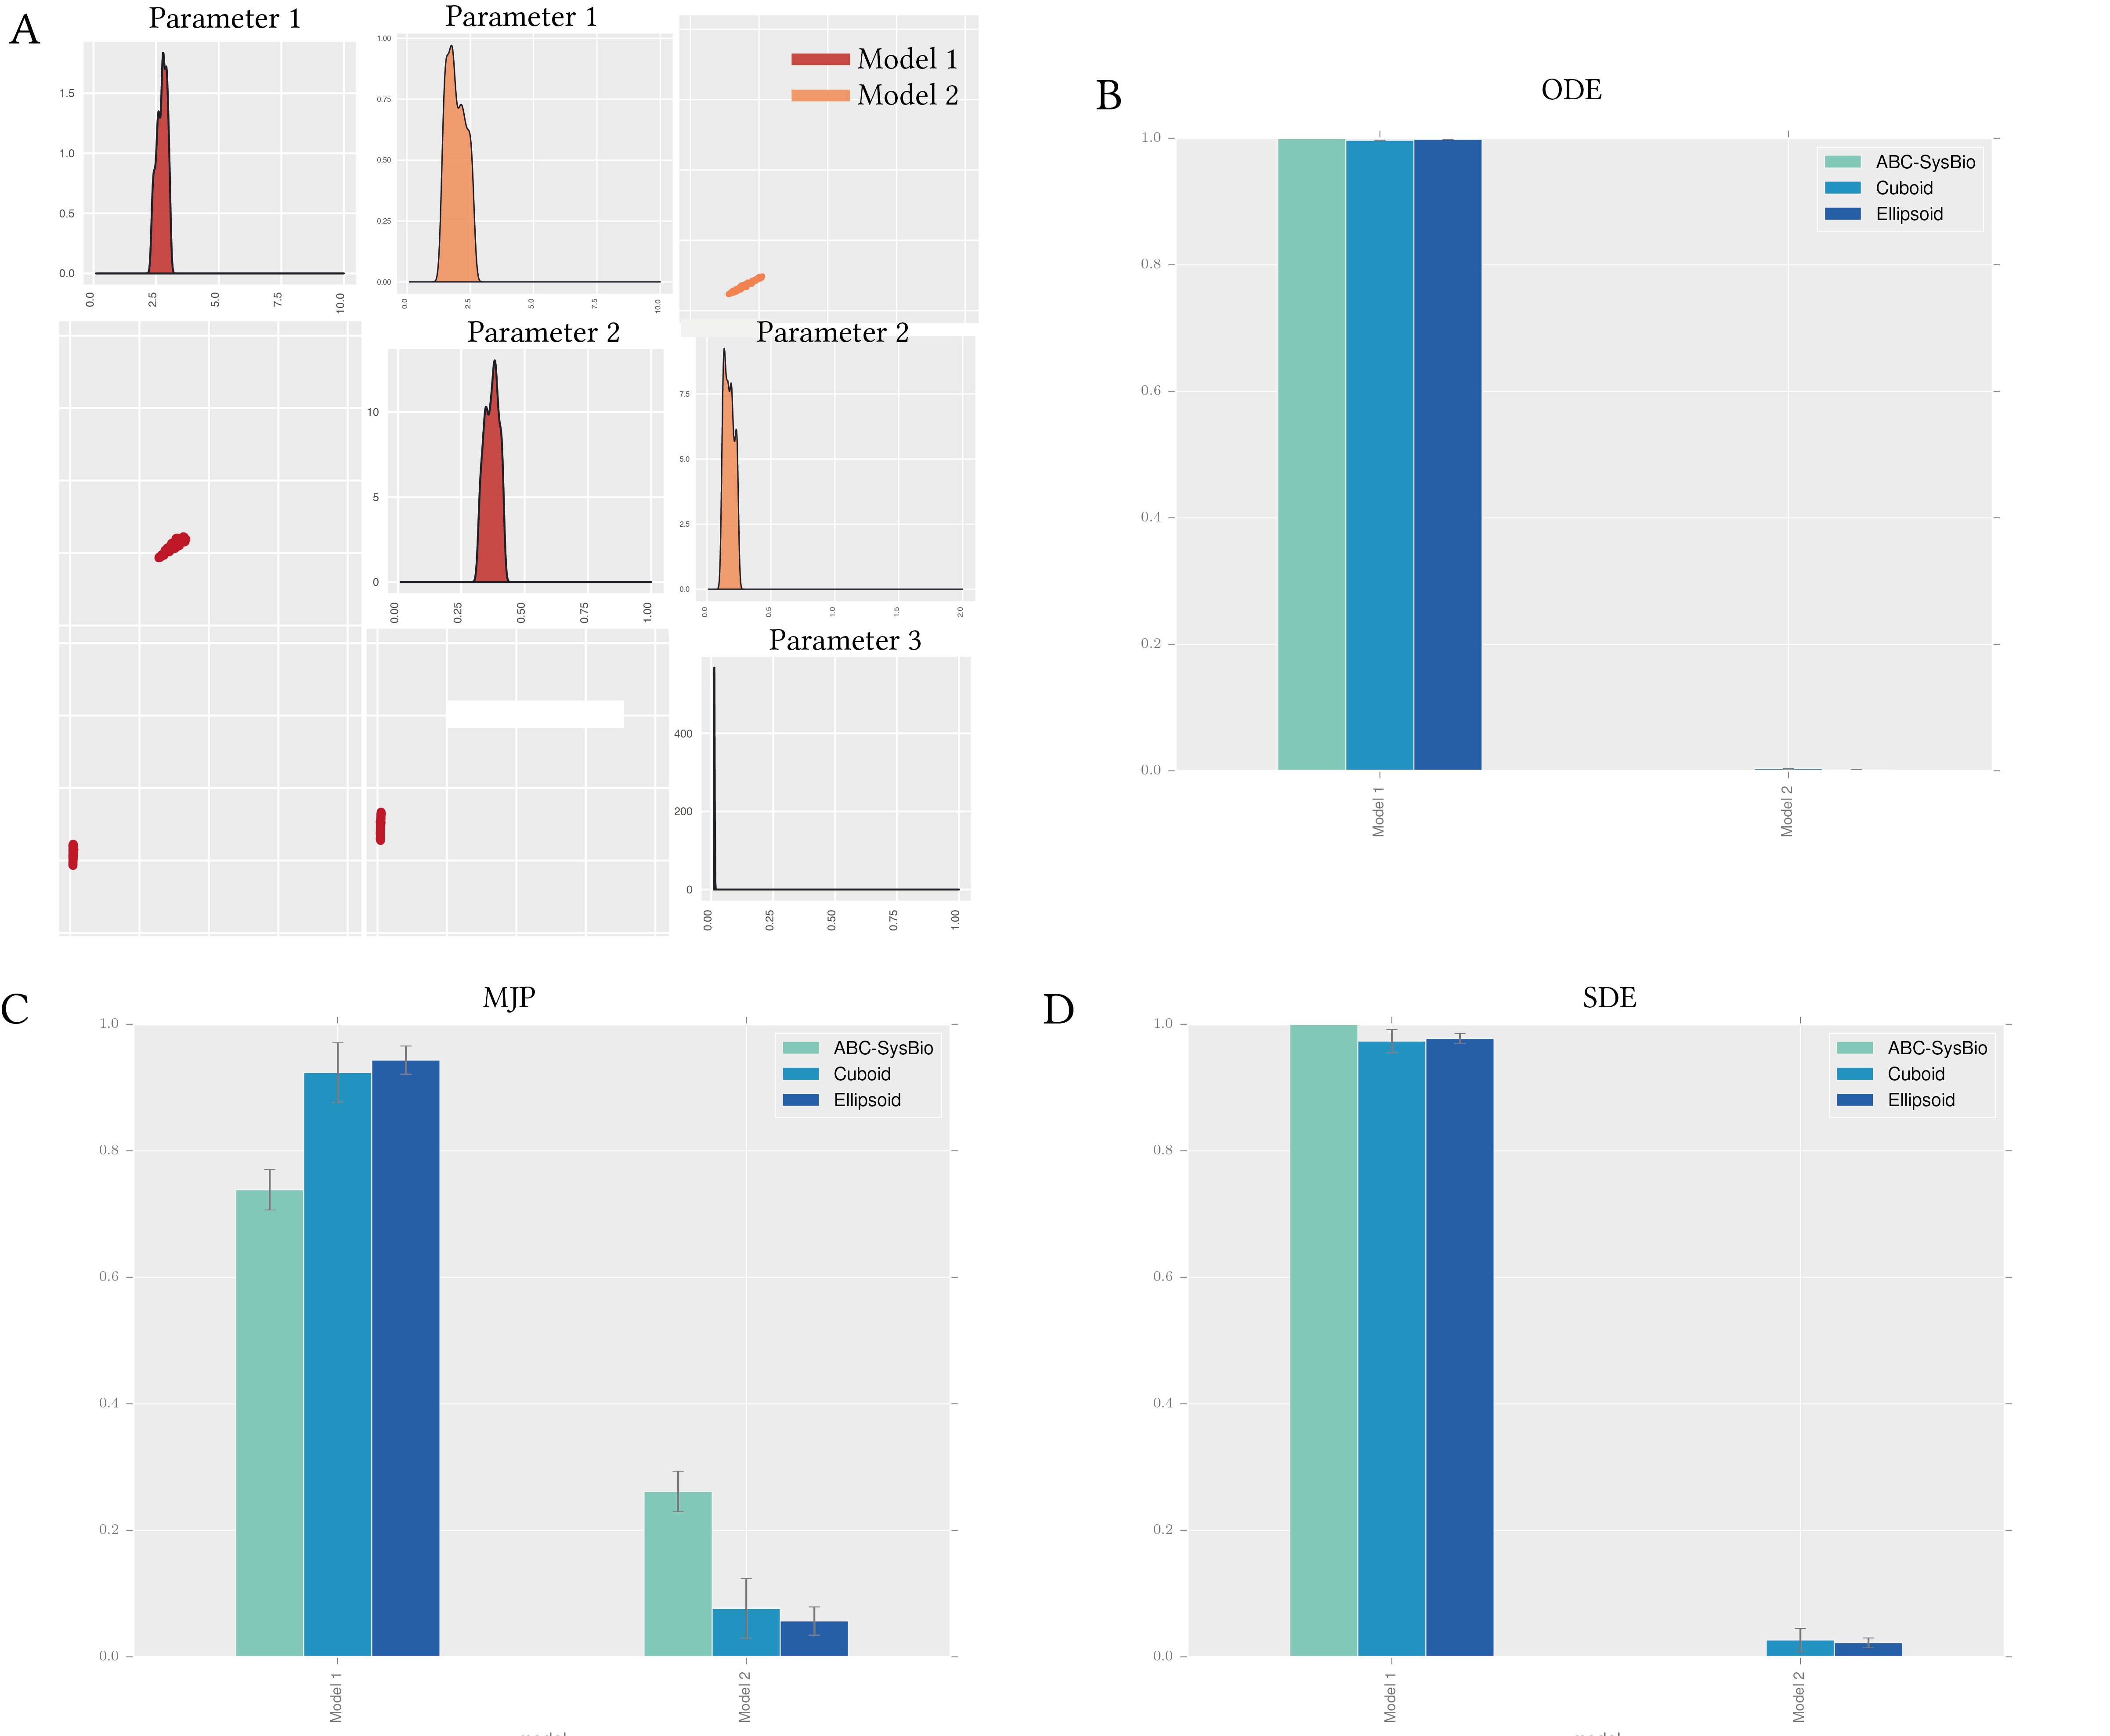
\includegraphics[width=\textwidth]{../../chapters/chapterStabilityFinder/images/ex4_summ.png}
\caption[Robustness analysis of case study 2]{\label{fig:rob_sysbio4}: Robustness comparison of two population growth models. (A) The posterior distributions of the two models. (B-D) The models were simulated using \acrshort{ode},~\acrshort{mjp} and~\acrshort{sde}. Both the cuboid and the ellipsoid approximations agree with ABC-SysBio model selection results. Each analysis was repeated three times. The height of the bars indicate the mean robustness from the three repeats and the error bars represent the standard deviation. }
\end{center}
\end{figure*}

\clearpage


The two case studies used above show that the cuboid and the ellipsoid approximation of model robustness agree with the results obtained from ABC-SysBio model selection. A point I must draw attention to is that for ABC-SysBio model selection where model selection is incorporated in the process, each model is also considered a particle with an associated weight~\autocite{Toni:2009tr}. If a model is performing poorly it does not proceed in the algorithm and is dropped when the weight falls low enough so that the model is not sampled~\autocite{Toni:2009tr}. This can save time in the analysis as computational resources are not wasted on 'dead' models, models that perform the required behaviour poorly. Using StabilityFinder for model selection, each model must reach the given final \textepsilon{} in order for the cuboid and ellipsoid methods to be valid. This means that time and computational power will be spent on models that are potentially a bad fit, or that have posterior distributions so small compared to the prior that it will take a long time for StabilityFinder to find it. Despite this, the results agree between the all three methods of model selection. This shows that the requirement for all models to reach the final \textepsilon{} does not affect the results for the models used in the above case studies. The potentially wasted computational resources on 'dead' models is a compromise made in order to be able to run the models separately, as model selection is not the primary purpose of StabilityFinder. 

\section{Applications of StabilityFinder}

In this section I apply StabilityFinder to switch models in order to find the design principles underlying their stabilities. First I apply it to a simple model with known results, the~\textcite{Gardner:2000vha} toggle switch. This model can serve as a test for StabilityFinder, as the conditions for bistability are derived in~\textcite{Gardner:2000vha}.


\subsection{StabilityFinder used on the Gardner toggle switch}
\label{sec:gard}
\textcite{Gardner:2000vha} constructed the first synthetic genetic toggle switch~\autocite{Gardner:2000vha}. Their model consisted of two mutually repressing transcription factors, as shown in Figure~\ref{fig:gard_mod}A, and in the deterministic case is defined by the following \acrshort{ode}s:

\begin{align}
\frac{du}{dt} &= \frac{a_1}{1+v^{\beta}} - u\\
\frac{dv}{dt} &= \frac{a_2}{1+u^{\gamma }} - v,
\end{align}
\noindent where \textit{u} is the concentration of repressor 1, \textit{v} the concentration of repressor 2, $a_1$ and $a_2$ denote the effective rates of synthesis of repressors 1 and 2 respectively, β is the cooperativity of repression of promoter 1 and γ of repressor 2. \textcite{Gardner:2000vha} studied the deterministic case and concluded that there are two conditions for bistability for this model; that $a_1$ and $a_2$ are balanced and that β, γ \textgreater 1 \autocite{Gardner:2000vha}. I test StabilityFinder by using it to find the posterior distribution for which this model exhibits bistable behaviour. Therefore, the desired behaviour is set to two steady states, and using a wide range of values as priors as shown in Table~\ref{tab:gard_det_stoch}, I used StabilityFinder to find the parameter values necessary for bistability to occur. The posterior distribution calculated by StabilityFinder for the Gardner deterministic case is shown in Figure~\ref{fig:gard_post}A.

\begin{table}[htbp]
\centering
\caption{Gardner switch priors in the deterministic and stochastic cases}
\label{tab:gard_det_stoch}
\begin{tabular}{@{}cccccc@{}}
\toprule
\multicolumn{4}{c}{Parameters (time\textsuperscript{-1})}                          & \multicolumn{2}{c}{Species (μM)} \\ \cmidrule(lr){1-4}
\cmidrule(lr){5-6}
$a_1$ & $\beta$ & $a_2$ & \multicolumn{1}{c}{$\gamma$} & $s_1$        & $s_2$        \\
0-60  & 0-5     & 0-60  & 0-5                           & 0-100        & 0-100        \\ \bottomrule
\end{tabular}
\end{table}

These results agree with the results reported by~\textcite{Gardner:2000vha}. For this switch to be bistable $a_1$ and $a_2$ must be balanced while β and γ must both be \textgreater 1, as can be seen in the marginal distributions of β and γ in Figure~\ref{fig:gard_post}A.

I next applied StabilityFinder to the case of the Gardner switch under stochastic dynamics using the same priors as the deterministic case, and again searched the parameter space for bistable behaviour. The posterior distribution is shown in Figure~\ref{fig:gard_post}B. We can see that the conditions on the parameters required for bistability in the deterministic case generally still stand in the stochastic case. There appears to be slightly looser requirements on the parameters of the stochastic model (wider marginal distributions). Some difference between the deterministic and stochastic posteriors is expected as different clustering algorithms are used for the stochastic and the deterministic cases. The Gap statistic is used in the case of the stochastic case, as it is capable of dealing with noisier data whereas a simpler and faster algorithm is used for clustering the deterministic solutions. These results demonstrate that StabilityFinder can be used to find the parameter values that can produce a desired stability and can be confidently applied to more complex models.


\begin{figure*}[htbp]
\begin{center}
	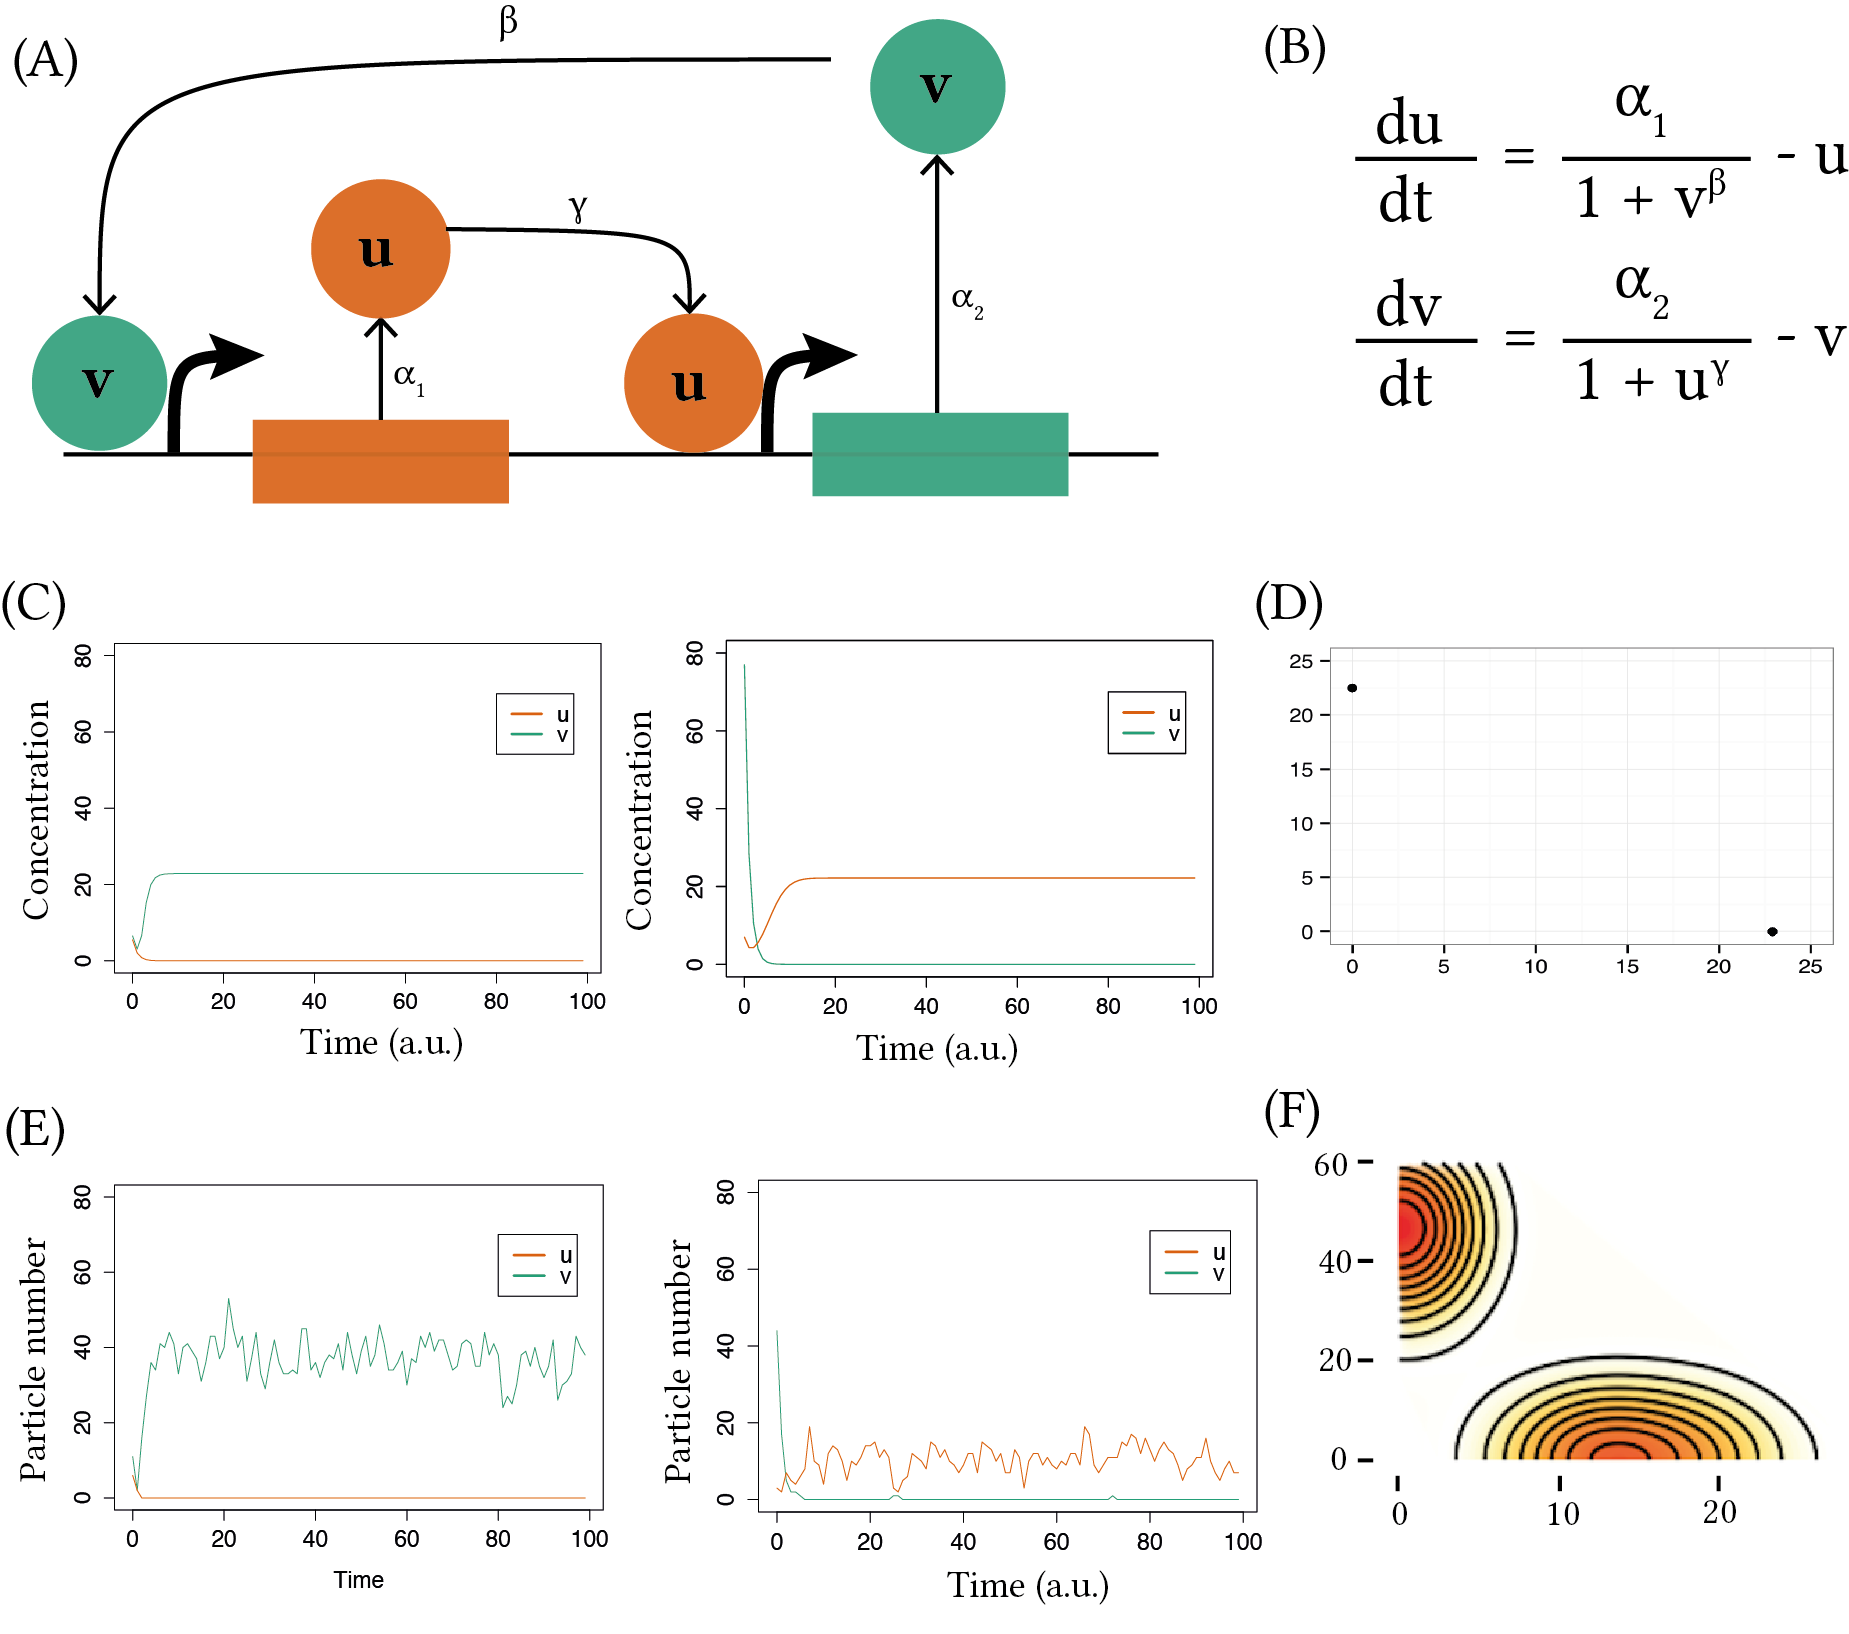
\includegraphics[scale=0.8]{../../chapters/chapterStabilityFinder/images/gardner_model.png}
	\caption[StabilityFinder used on the Gardner toggle switch]{\label{fig:gard_mod} The Gardner switch model used to test StabilityFinder. The Gardner model (A) consists of two mutually repressing transcription factors. It can be reduced to a two-equation system (B) , where $u$ and $v$ are the two transcription factors, $a_1$,$a_2$ are their effective rates of synthesis, $u$,$v$ are their concentrations and $\beta$, $\gamma$ represent the cooperativity of each promoter. (C) Two samples of deterministic simulated timecourses of the Gardner switch and (D) The resulting phase plot. (E) Two samples of timecourses of the stochastic simulations and (F) the resulting stationary distributions.}
\end{center}
\end{figure*}

\begin{figure*}[htbp]
\begin{center}
	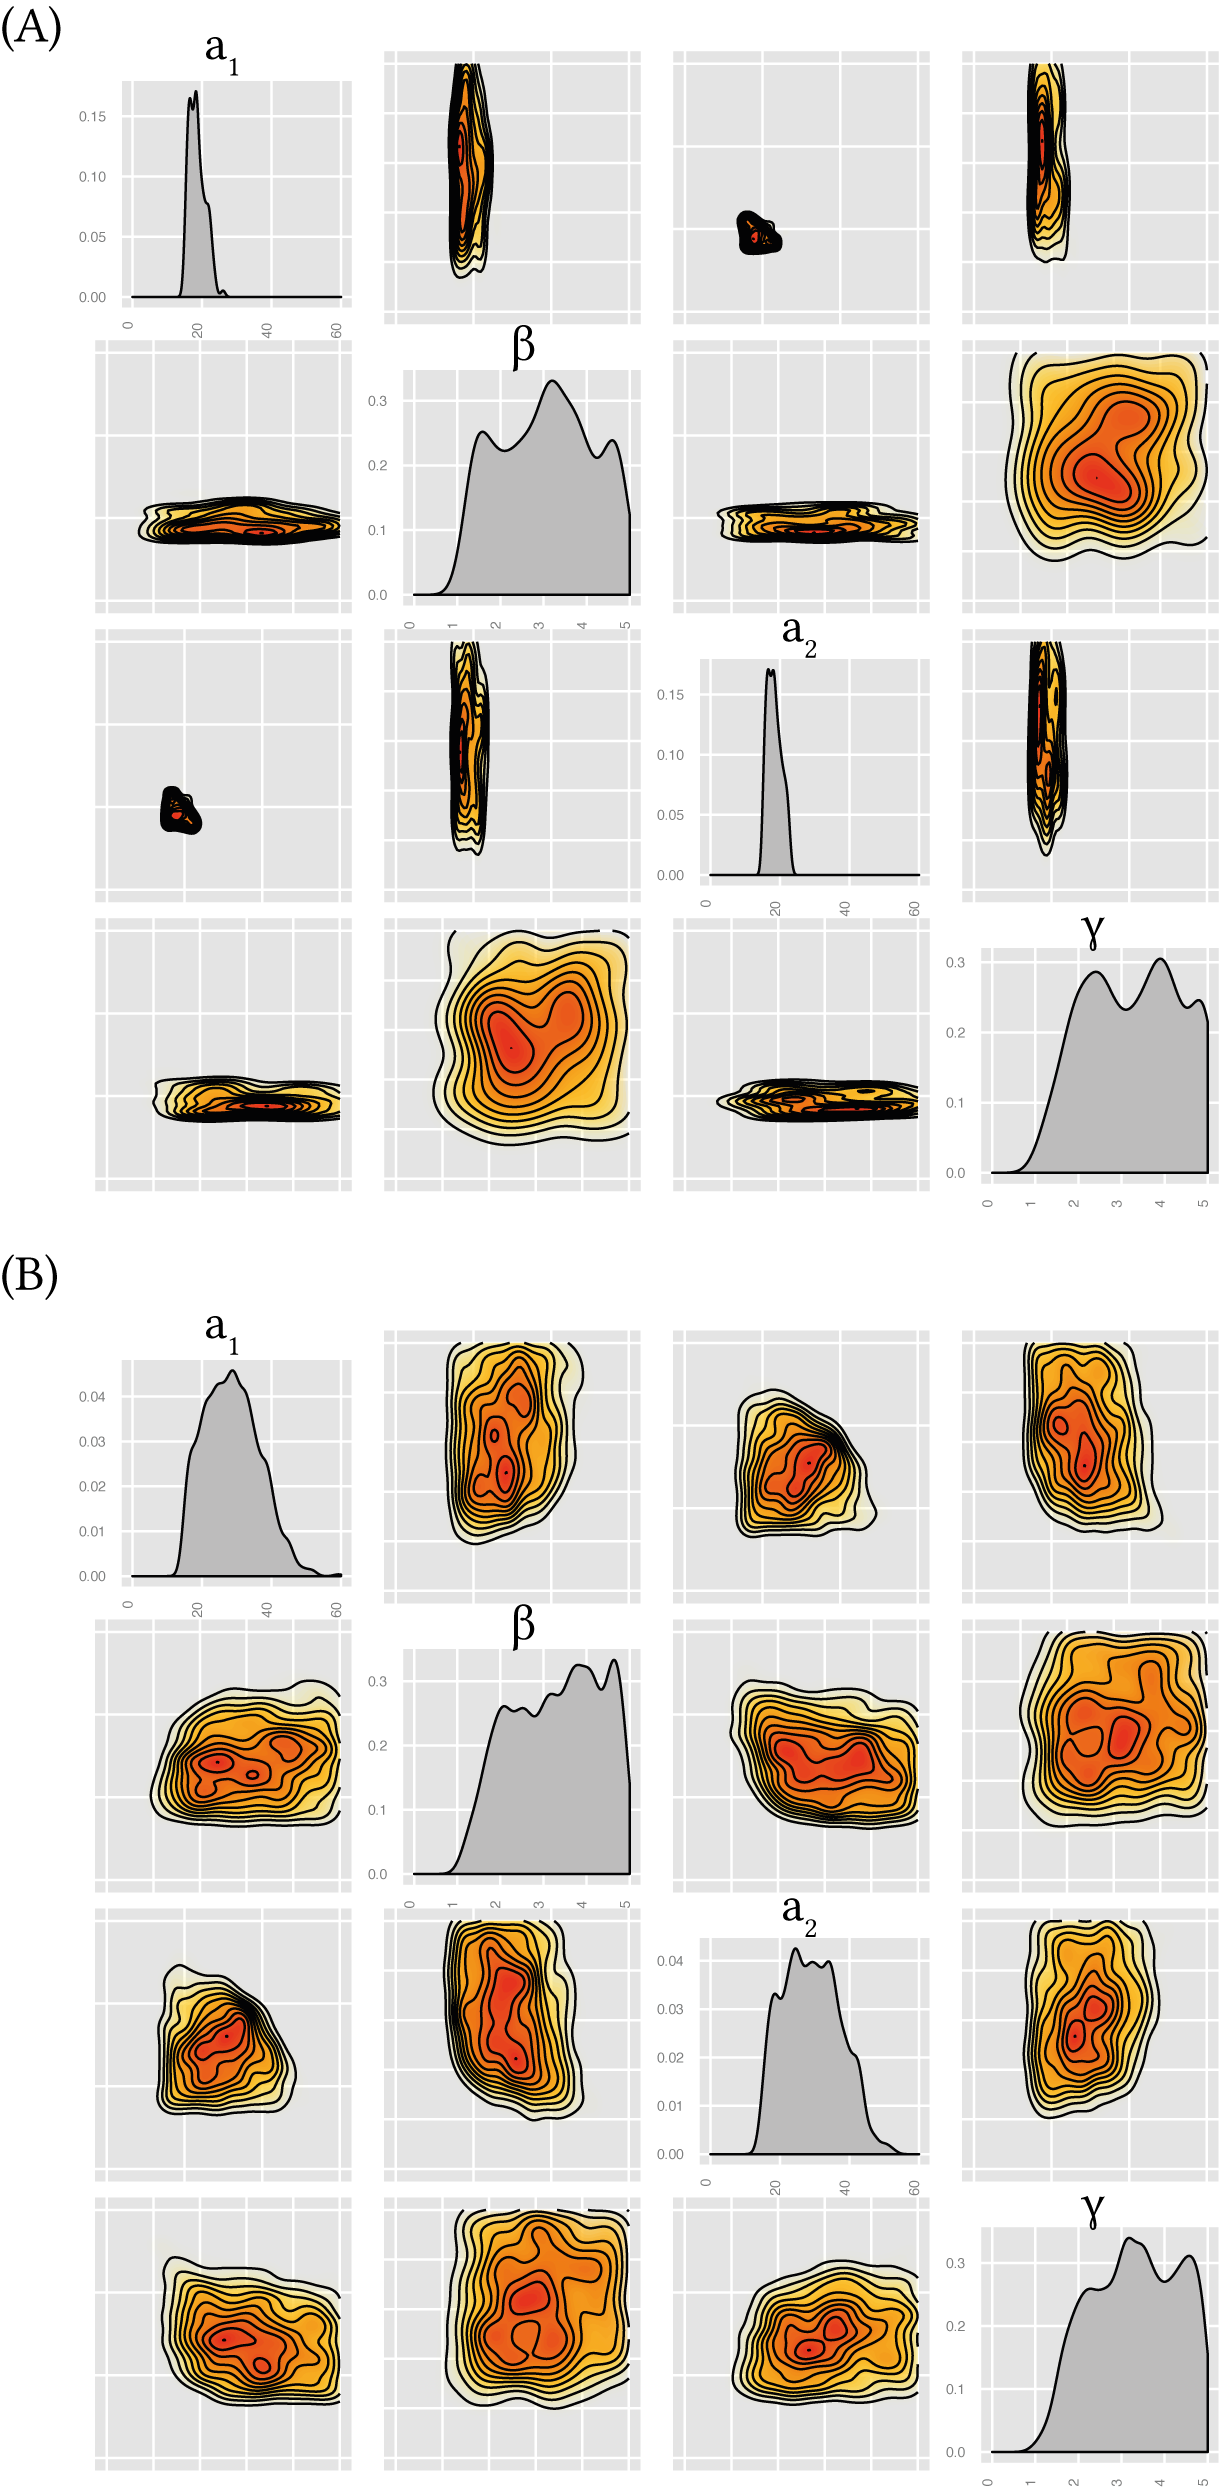
\includegraphics[scale=0.8]{../../chapters/chapterStabilityFinder/images/gardner_posteriors.png}
	\caption[The posterior distributions of the bistable Gardner toggle switch]{\label{fig:gard_post} Elucidating the stability of the Gardner switch. The Gardner model has four parameters, for which I want to find the values for which this system is bistable. I use StabilityFinder to find the posterior distribution of the bistable Gardner switch, deterministically (A) and stochastically (B). The posterior distributions are shown as the density plots of each parameter as well as each one plotted against the other.  }
\end{center}
\end{figure*}
\clearpage
%\begin{figure*}[h]
%\begin{center}
%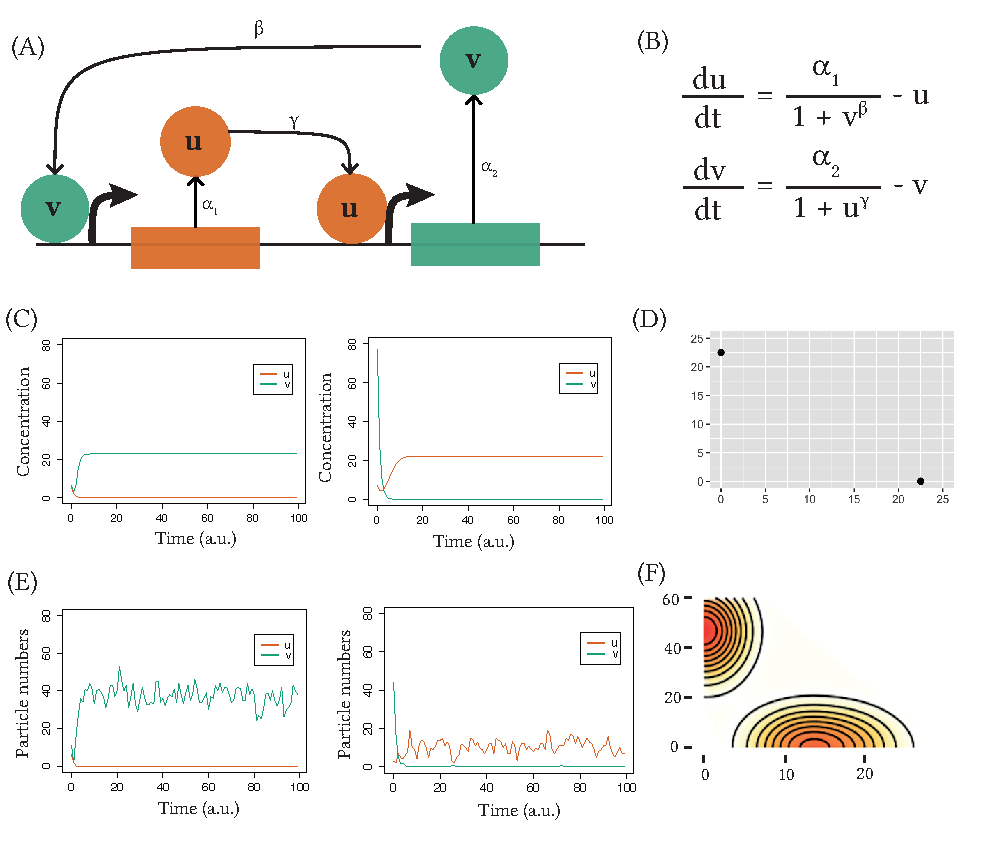
\includegraphics[width=\textwidth]{../../chapters/chapterStabilityFinder/images/gardner_poster.png}
%\caption[LoF caption]{ \label{fig:fig2}: Elucidating the stability of the Gardner switch. The Gardner model (A) consists of two mutually repressing transcription factors. It can be reduced to a two-equation system, where $u$ and $v$ are the two transcription factors, $a_1$,$a_2$ are their effective rates of synthesis, $u$,$v$ are their concentrations and $\beta$, $\gamma$ represent the cooperativity of each promoter. There are four parameters in the model, for which we want to find the values for which this system is bistable. We use StabilityFinder to find the posterior distribution of the bistable Gardner switch, deterministically (B) and stochastically (C). The posterior distributions are shown as the density plots of each parameter as well as each one plotted against the other. }
%\end{center}
%\end{figure*}
%\clearpage


\subsection{Lu toggle switch models}
\label{sec:lu}
Next I analyzed an extension of the Gardner switch model developed by~\textcite{Lu:2014kc}. I use these models as they are of increased complexity from the Gardner model. \textcite{Lu:2014kc} considered two types of switches, the classic switch consisting of two mutually repressing transcription factors (model \acrshort{cs-lu}), as well as a double positive switch \acrshort{dp-lu}.  The \acrshort{cs-lu} switch was found to be bistable given the set of parameters used, while the \acrshort{dp-lu} switch was found to be tristable~\autocite{Lu:2014kc}. The \acrshort{cs-lu} model used in their study is given by the following system of \acrshort{ode}s, as given in~\textcite{Lu:2014kc}.

\begin{align}
\dot{x} & = g_{x}\, H^{S}_{xy}(y) -k_{x}x \\
\dot{y} & = g_{y}\,H^{S}_{yx}(x) -k_{y}y,
\end{align}

\noindent where:

\begin{align}
H^{S}_{I}(x) &= H^{-}_{I}(x)+\lambda_{I}H^{+}_{I}(x) \\
H^{-}_{I}(x) &= 1 \big/\left[1+(x/x_{I})^{n_{I}}\right] \\
H^{+}_{I}(x) &= 1-H^{-}_{I}(x),
\end{align}

\noindent and the \acrshort{dp-lu} model is given by
\begin{align}
\dot{x} = f_{x}(x,y) &= g_{x}\, H^{S}_{xy}(y)\, H^{S}_{xx}\,(x)-k_{x}x \\
\dot{y} = f_{y}(x,y) &= g_{y}\,H^{S}_{yx}(x)\,H^{S}_{yy}\,(y)-k_{y}y,
\end{align}

\noindent $g_I$ represents the production rate, $k_I$ the degradation rate, $n_I$ the Hill coefficient, $x_I$ the Hill threshold concentration and $\lambda_I$ the fold change of the transcription rates, and $I\in\{xy, yx, xx, yy\}$.

For the parameter values used in the Lu study, the \acrshort{cs-lu} switch exhibits three steady states, two of which are stable and one is unstable. The \acrshort{cs-lu} switch exhibits five steady states, of which three are stable and two are unstable. Bifurcation diagrams of the two Lu models are shown in Figure~\ref{fig:lu_bifurc}. 


\begin{figure*}[htbp]
\begin{center}
	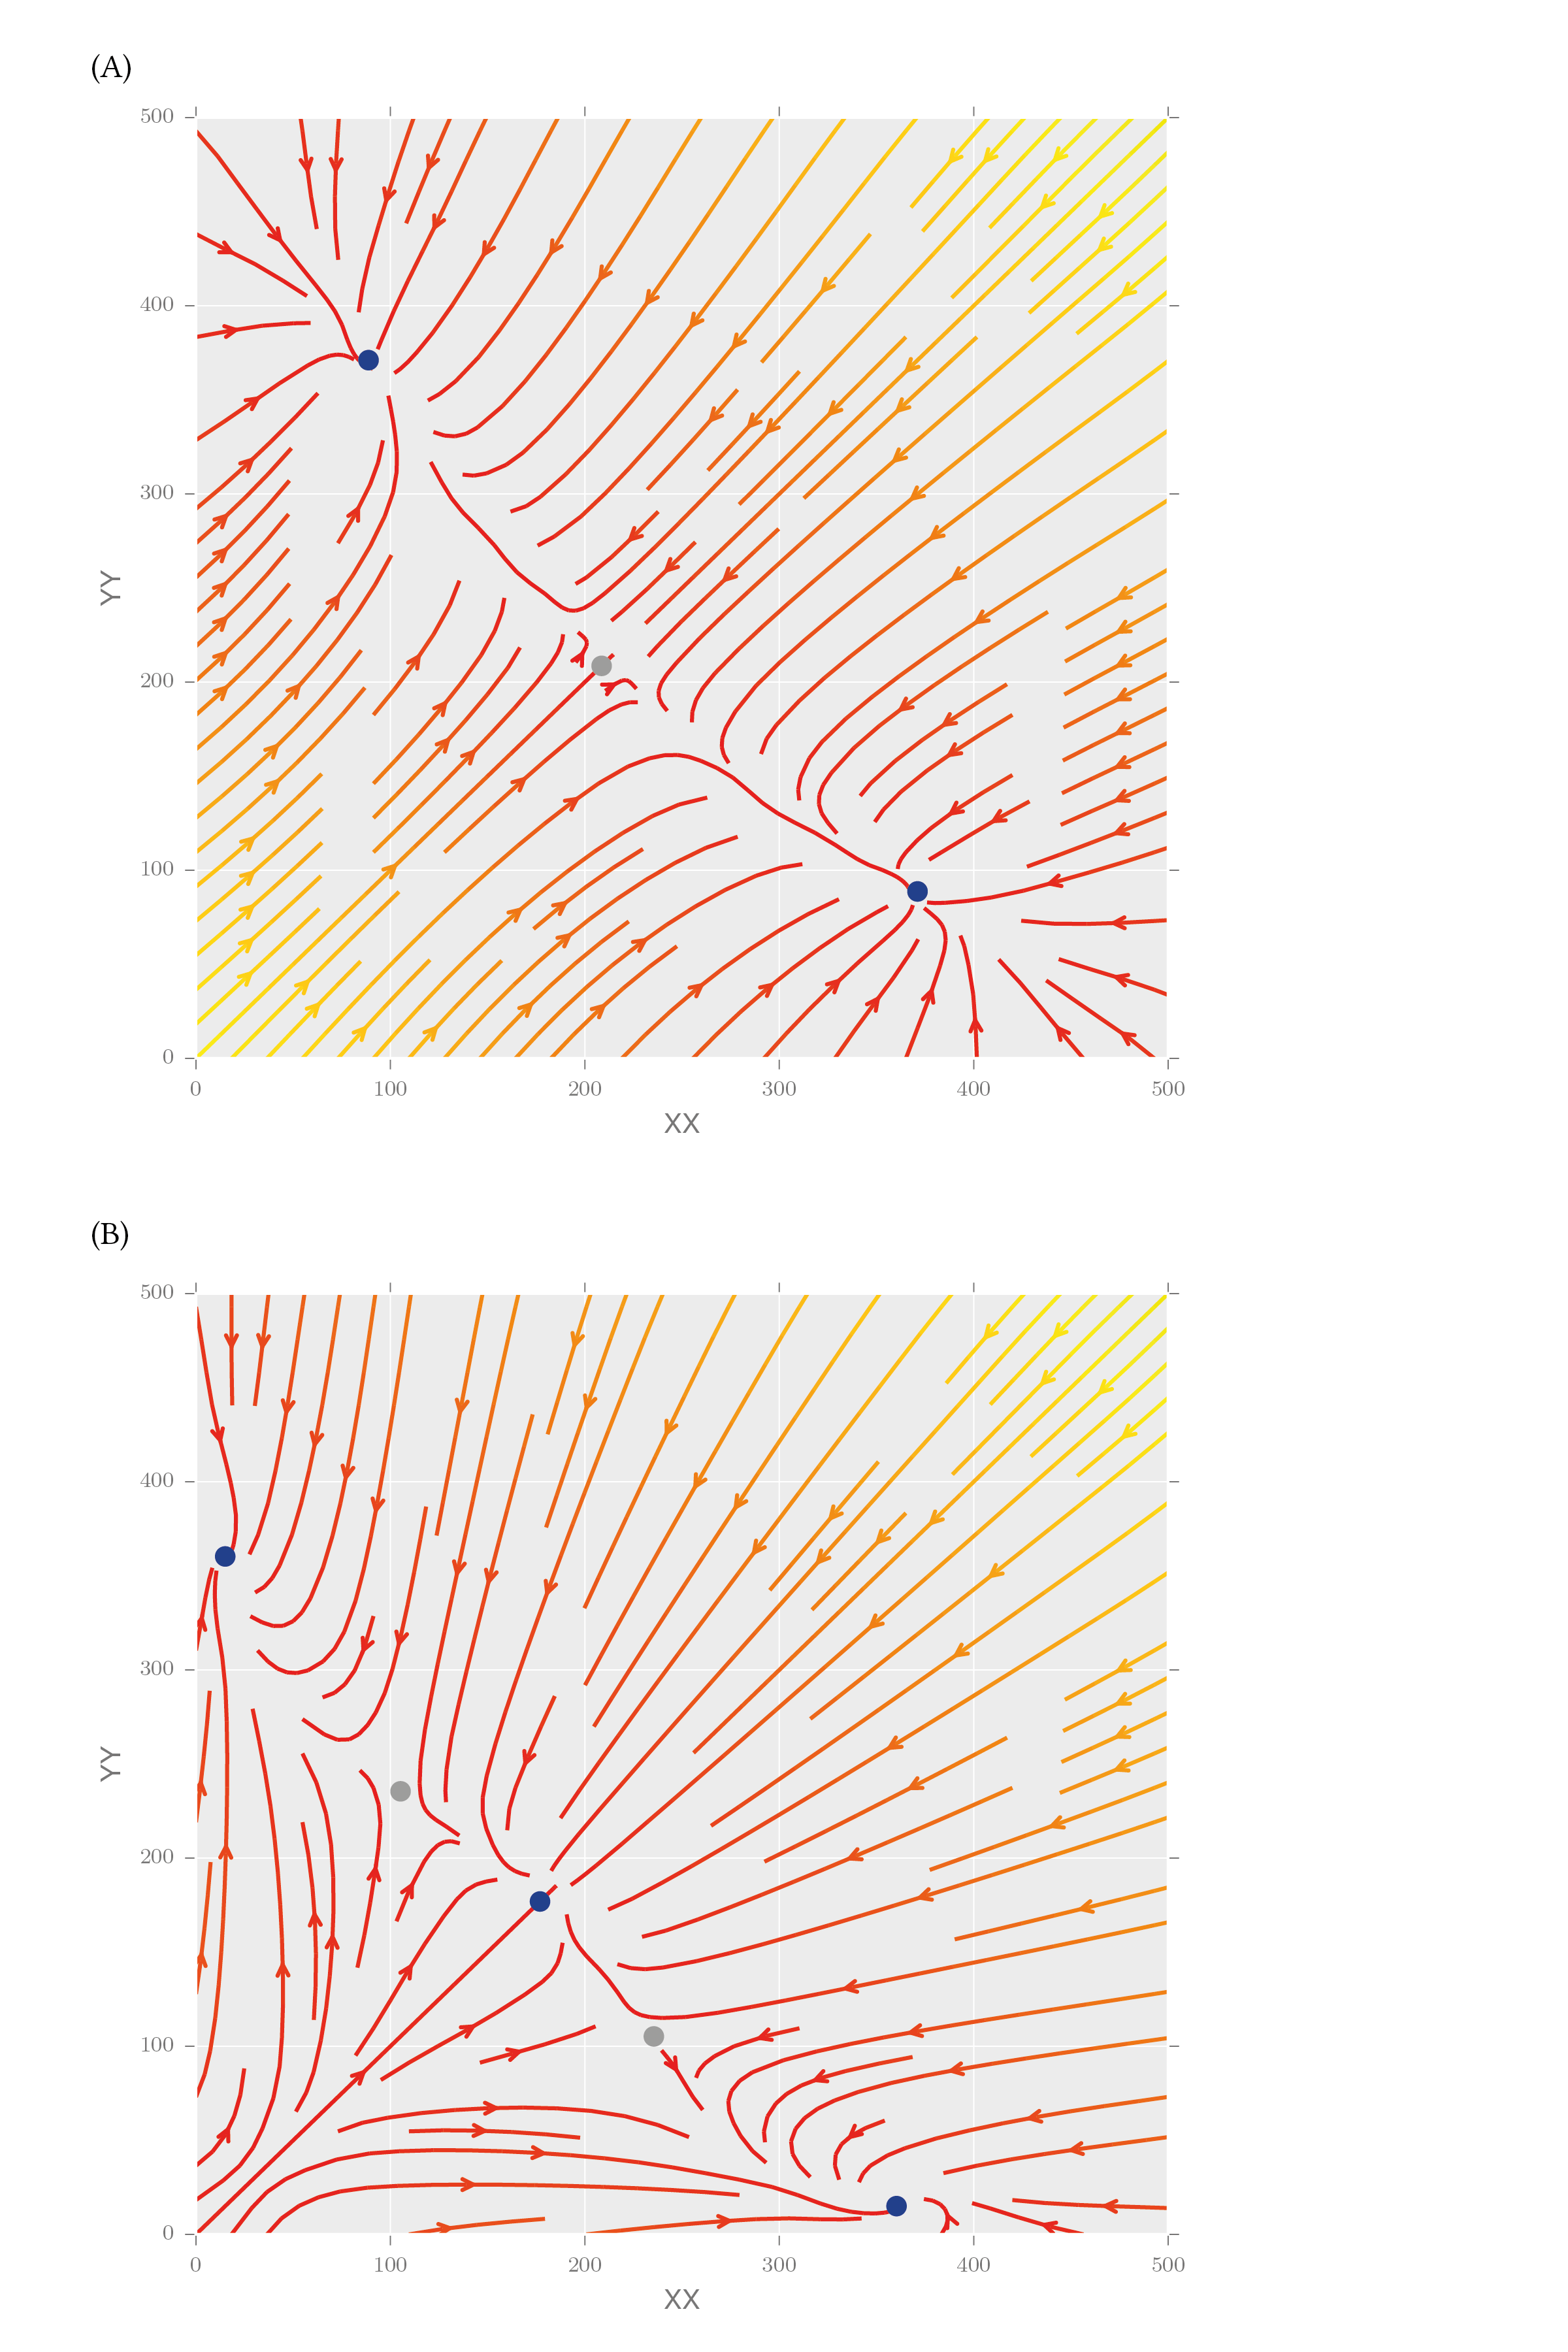
\includegraphics[scale=0.5]{../../chapters/chapterStabilityFinder/images/lu_bifurc.png}
	\caption[Phase plane analysis of the Lu toggle switch models]{\label{fig:lu_bifurc}  Stream plot of the vector plot of the (A) \acrshort{cs-lu} and \acrshort{dp-lu} switches. The colours indicate the magnitude of the vectors, with yellow indicating high and red low values. The blue points represent stable steady states and the grey points represent unstable steady states.  }
\end{center}
\end{figure*}
\clearpage
 
\subsubsection{Extending the Lu models}

I start the analysis of the Lu models by extending their analytical approach to solving the system. I use StabilityFinder to explore a larger parameter space which allows us to distinguish between rare events and robust behaviours. The advantage of using StabilityFinder over solving the system analytically is that the full parameter space is explored rather than solving the system for a single set of parameters. This allows us to deduce model properties that could not otherwise be identified. Robustness to parameter fluctuations can be explored, as well as parameter correlations and restrictions on the values they can take while still producing the desired behaviour. 

It is known that that the addition of positive autoregulation to the classical toggle switch can induce tristability~\autocite{Lu:2014kc}. Here I investigate the interplay of positive autoregulation on the values of the other parameters in the model. I extended the analysis presented in~\textcite{Lu:2014kc} by including the switch with single positive autoregulation (model \acrshort{sp-lu}), where an asymmetry of positive feedbacks is present between the two genes. The three switches considered in this analysis are shown in Figure~\ref{fig:lu_mods}.  


\begin{figure*}[tb]
\begin{center}
	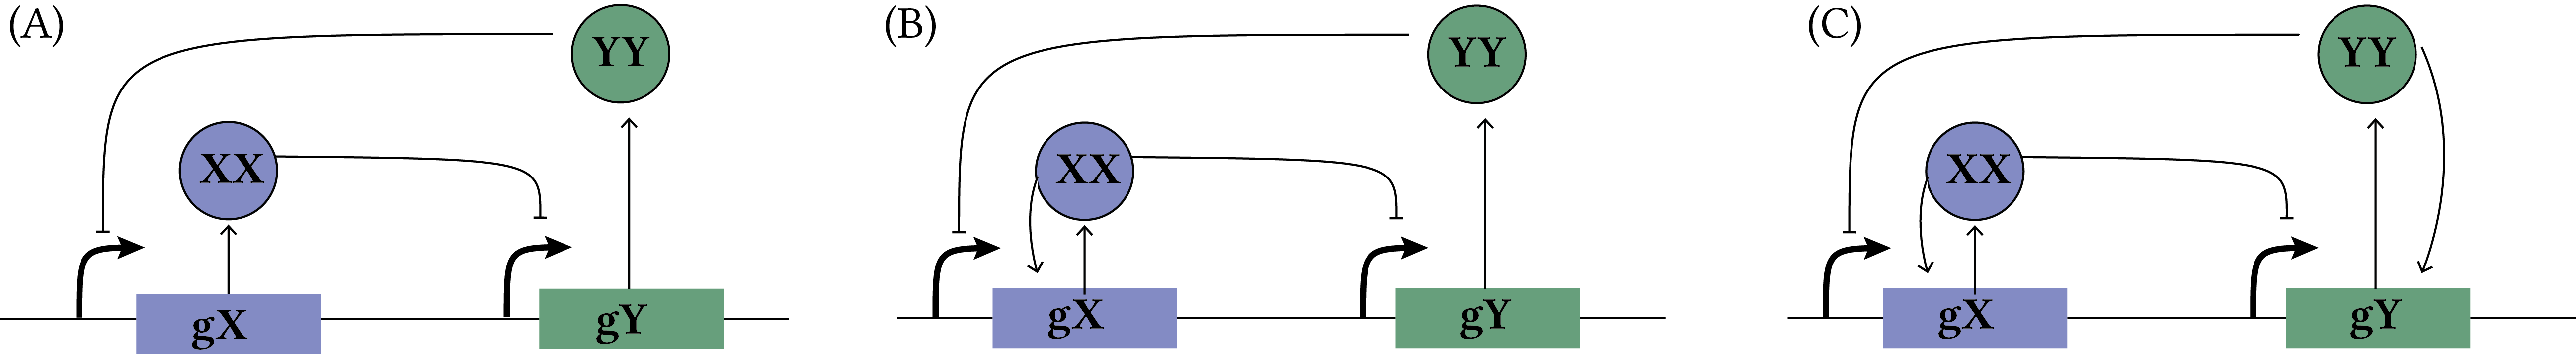
\includegraphics[width=\textwidth]{../../chapters/chapterStabilityFinder/images/LU_diagrams.png}
	\caption[The three Lu toggle switch models.]{\label{fig:lu_mods} The three LU toggle switch models. (A) \acrshort{cs-lu}, (B) \acrshort{sp-lu} and (C) \acrshort{dp-lu}.   }
\end{center}
\end{figure*}


The \acrshort{sp-lu} switch is modelled using the following \acrshort{ode} system
\begin{align}
\dot{x} & = g_{x}\, H^{S}_{xy}(y)\, H^{S}_{xx}\,(x)-k_{x}x \\
\dot{y} & = g_{y}\,H^{S}_{yx}(x) - k_{y}y.
\end{align}


Using StabilityFinder with priors centred around the parameter values used in the original paper (see Table~\ref{tab:lu_all}), we can identify the most important parameters for achieving the models' stability. The phase plots of the final populations of the models are shown in Figure~\ref{fig:lu_paper_phase} and the posterior distribution of these models are shown in Figure~\ref{fig:fig3}A. We find that the parameters representing the rates of degradation of the transcription factors in the system ($k_x$, $k_y$) must both be large in relation to the prior ranges for bistability to occur. Protein degradation rates have been shown to be important for many system behaviours including oscillations \autocite{Woods:2016eh}.

\begin{table}[htpb]
\centering
\caption{Priors of the classical (\acrshort{cs-lu}), single positive (\acrshort{sp-lu}) and double positive (\acrshort{dp-lu}) models.}
\label{tab:lu_all}
\begin{tabular}{@{}ccccc@{}}
\toprule
Parameter                                            & Symbol & \acrshort{cs-lu}        & \acrshort{sp-lu}         & \acrshort{dp-lu}       \\ \midrule
\multirow{2}{4cm}{Production rate (Proteins/Minute)}                & gx        & 30-50   & 1-2       & 1-100    \\
                                                & gy        & 30-50   & 20-25     & 1-100    \\[4pt]
\multirow{2}{4cm}{Degradation rate (Minute-1)}               & kx        & 0-0.5   & 50-55     & 0-1      \\
                                                & ky        & 0-0.5   & 48-52     & 0-1      \\[4pt]
\multirow{2}{4cm}{Hill coefficient}               & nxy       & 1-5     & 30-35     & 0-10     \\
                                                & nyx       & 1-5     & 0.1-0.2   & 0-10     \\[4pt]
\multirow{2}{4cm}{Hill thresholds concentration (Proteins)}  & xxy       & 100-300 & 2-3       & 100-1000 \\
                                                & xyx       & 100-300 & 0.4-0.6   & 100-1000 \\[4pt]
\multirow{2}{4cm}{Transcription rate fold change} & lxy       & 0-0.5   & 0.02-0.04 & 0-1      \\
                                                & lyx       & 0-0.5   & 0.02-0.04 & 0-0.2    \\[4pt]
\multirow{2}{4cm}{Hill coefficient}               & nXX       & -       & 25-30     & 0-10     \\
                                                & nYY       & -       & 0.01-0.02 & 0-10     \\[4pt]
\multirow{2}{4cm}{Hill thresholds concentration (Proteins)}  & xXX       & -       & 0.4-0.5   & 50-500   \\
                                                & xYY       & -       & 1-3       & 50-500   \\[4pt]
\multirow{2}{4cm}{Transcription rate fold change} & lXX       & -       & 65-72     & 1-20     \\
                                                & lYY       & -       & 0.02-0.04 & 1-20     \\ \hline
\end{tabular}
\end{table}



\begin{figure*}[p]
\begin{center}
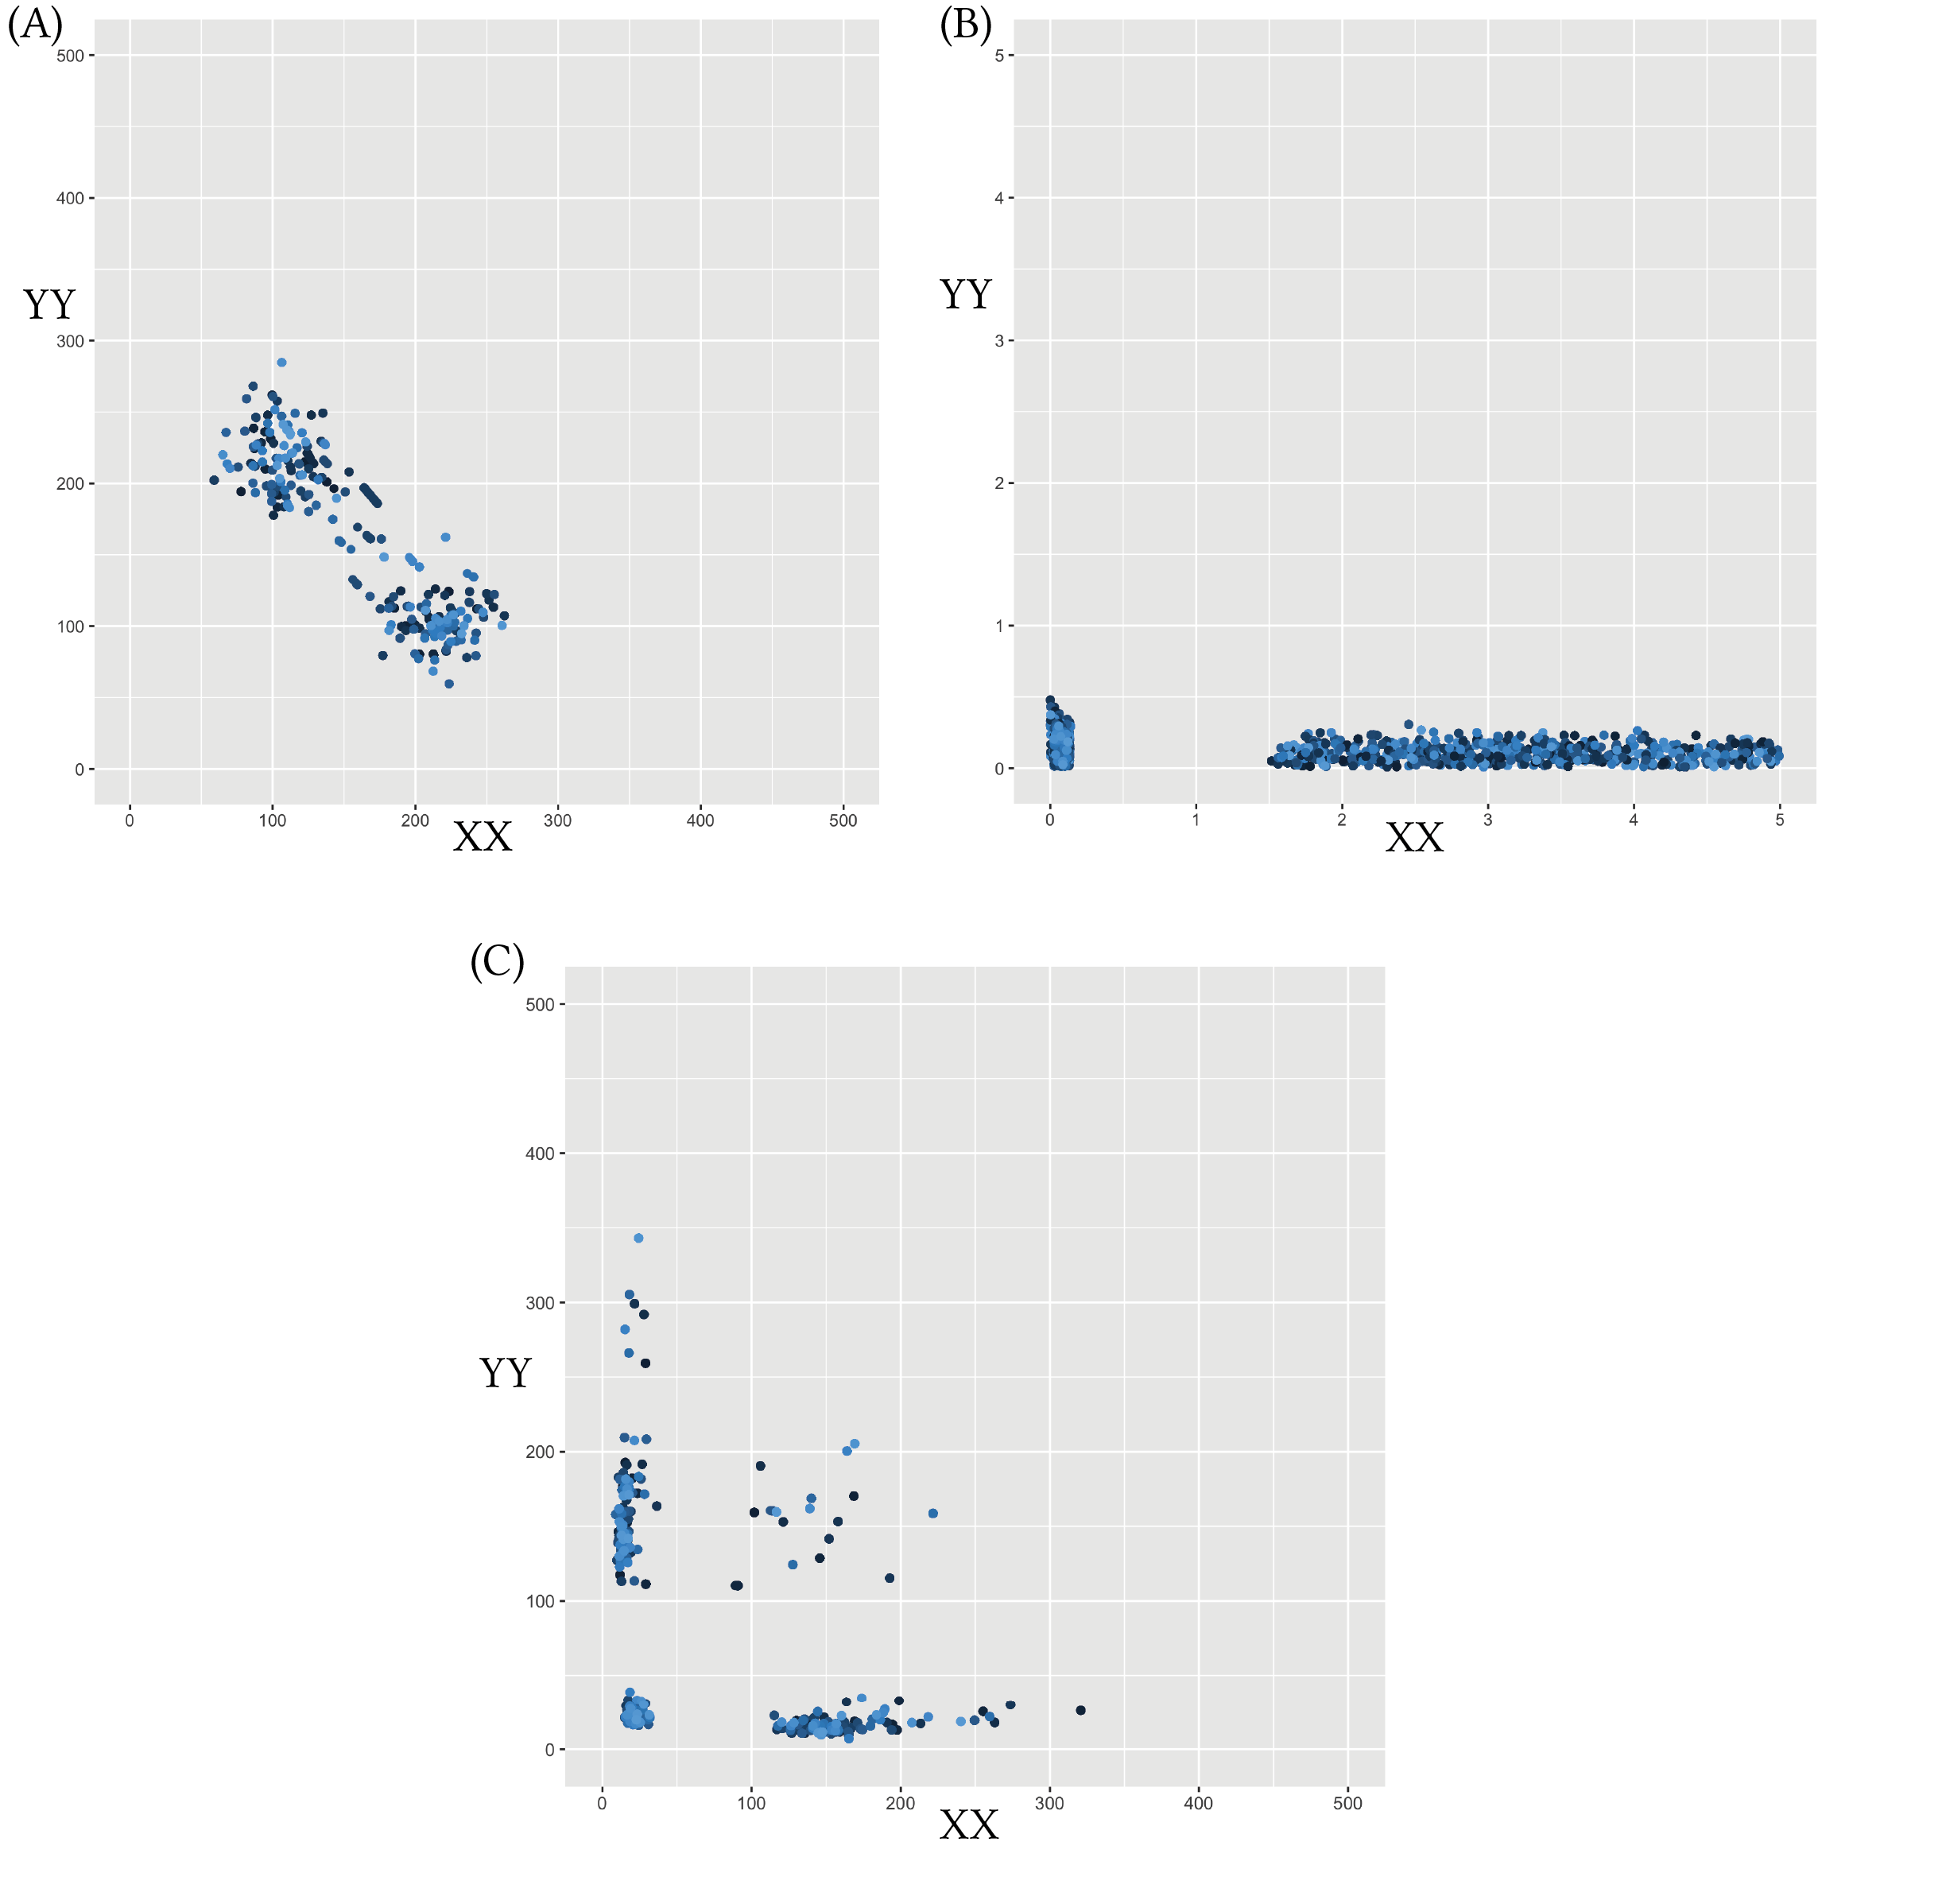
\includegraphics[width=\textwidth]{../../chapters/chapterStabilityFinder/images/lu_paper_phase.png}
\caption[Resulting phase plots from StabilityFinder used on the Lu switches ]{ \label{fig:lu_paper_phase}The phase plots of 100 particles from the last population of the three Lu switches. (A) The bistable \acrshort{cs-lu} (B) The bistable \acrshort{sp-lu} and (C) The tristable \acrshort{dp-lu}. We find two types of tristable behaviour, one where the third steady state is zero-zero and one where the third state is high (non-dead). }
\end{center}
\end{figure*}
\clearpage

\begin{figure*}[p]
\centerfloat
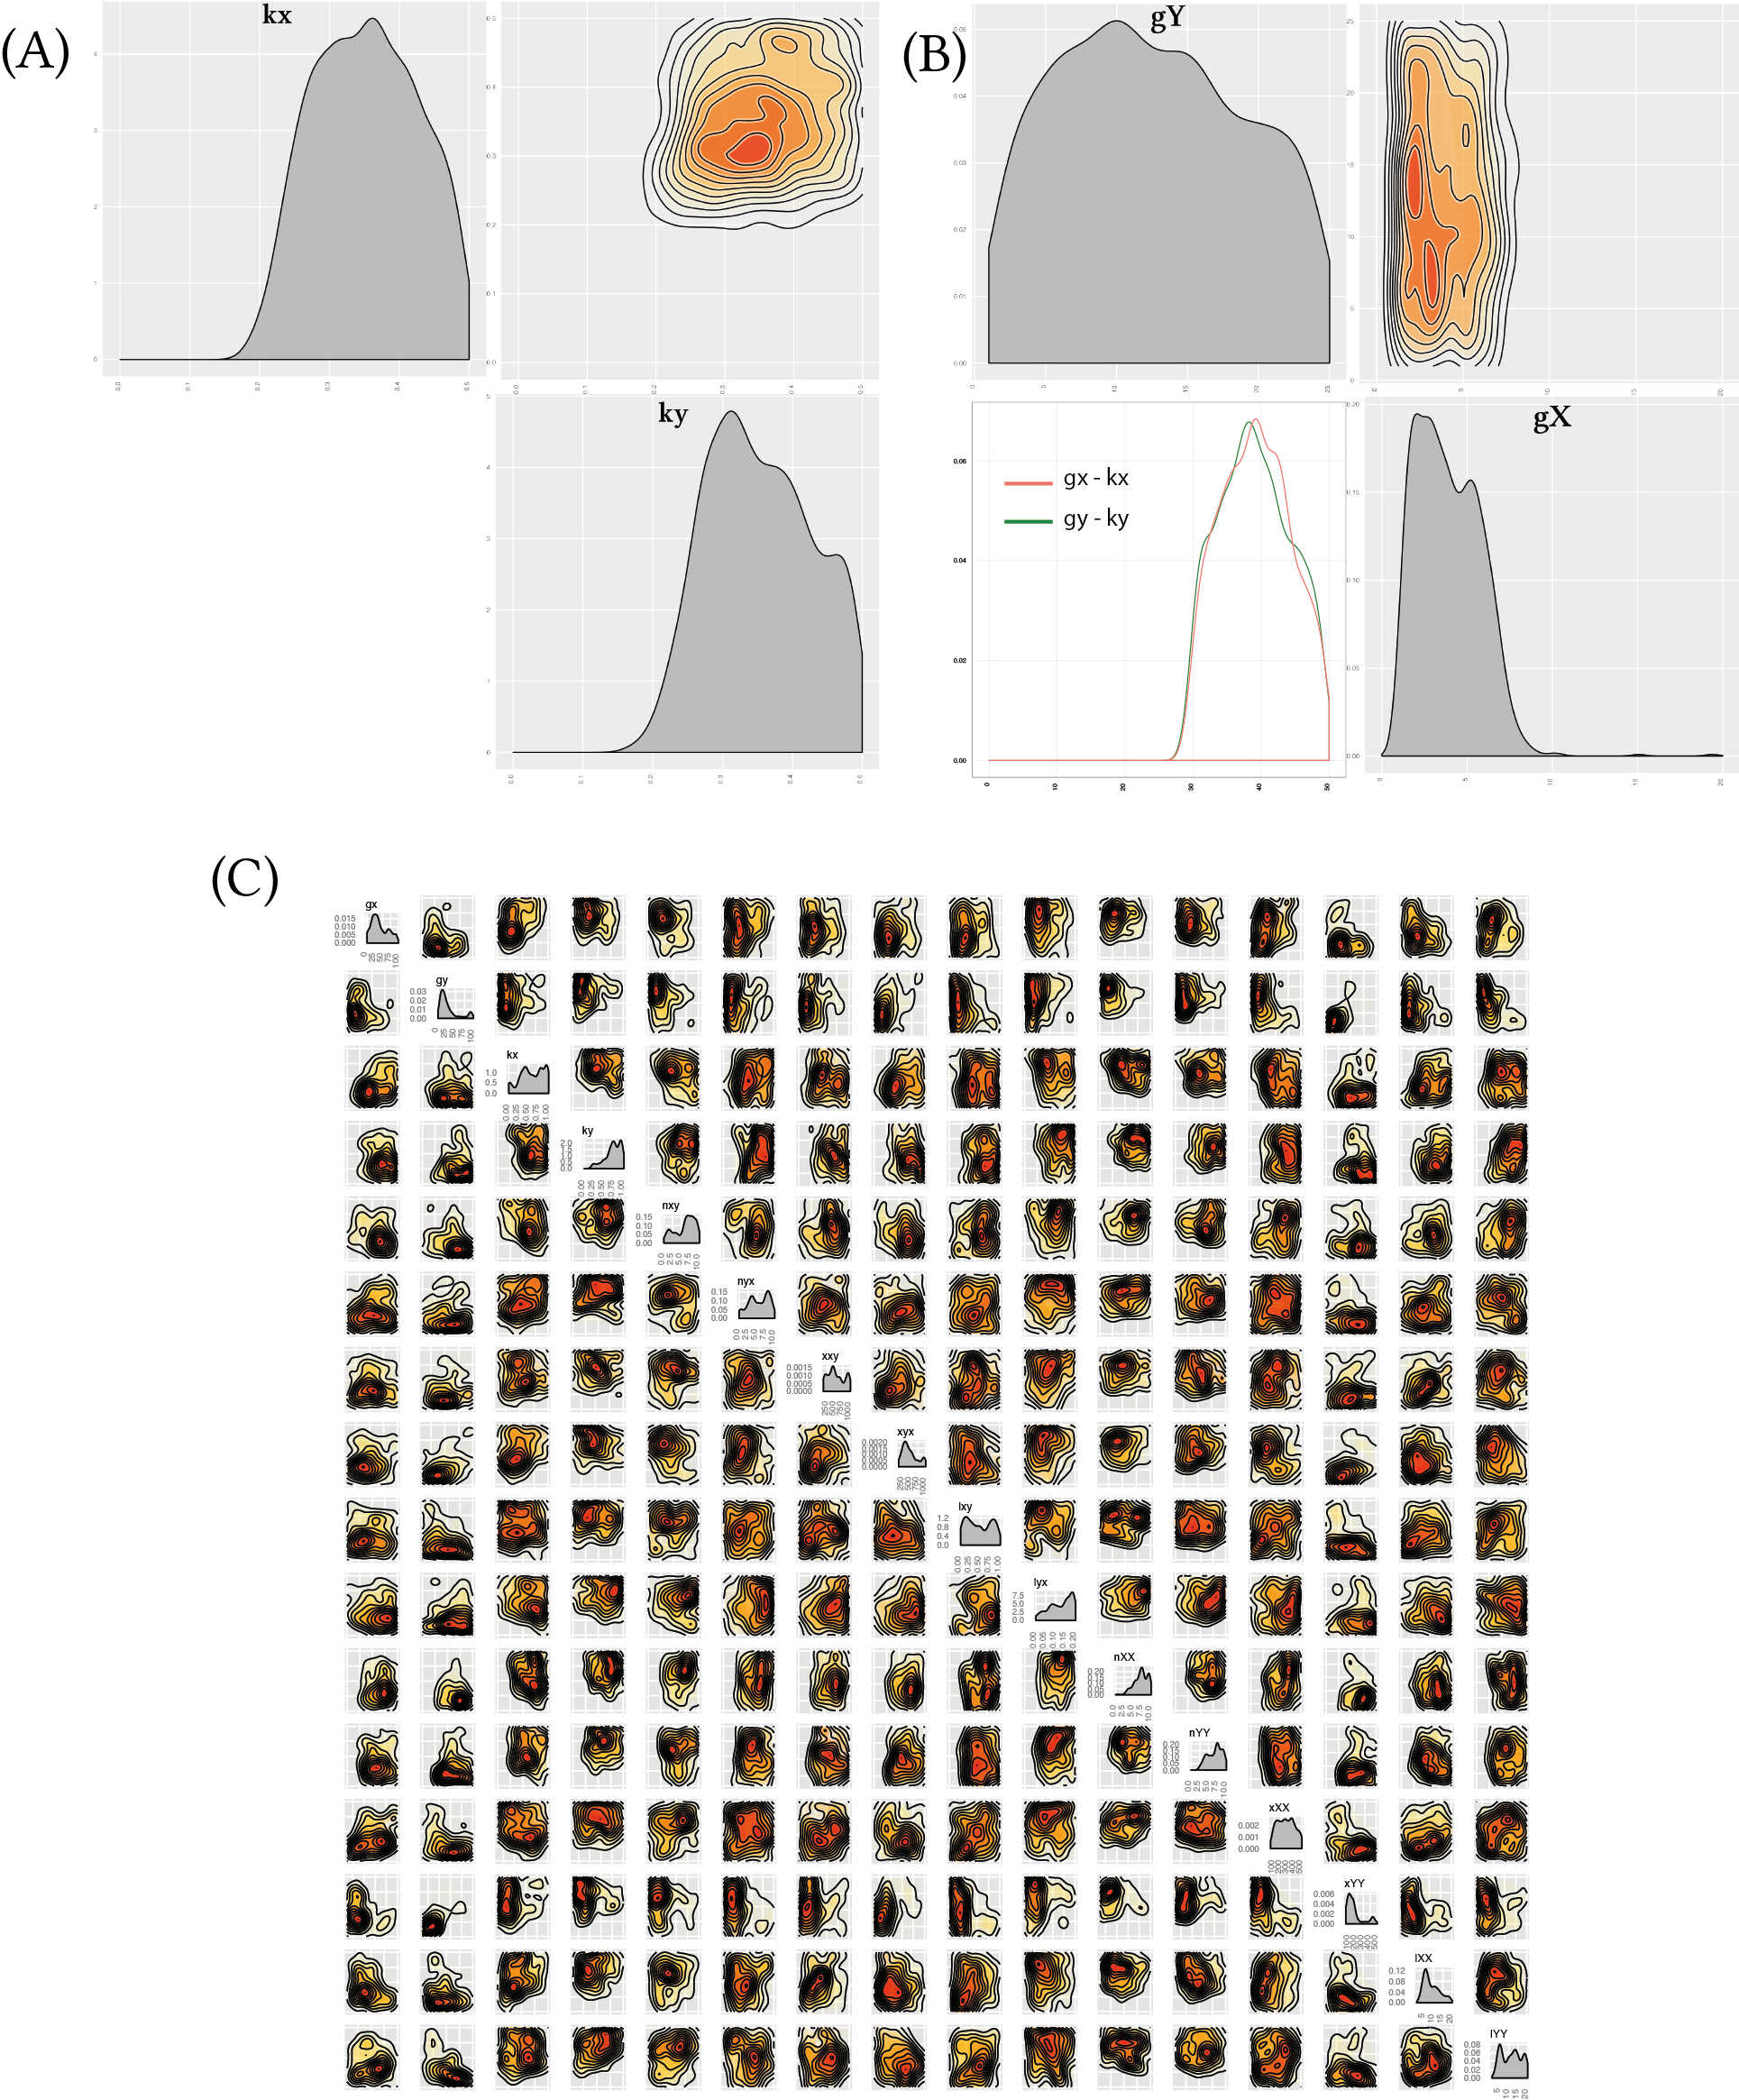
\includegraphics[width=1.3\textwidth]{../../chapters/chapterStabilityFinder/images/lu_paper_post.png}
\caption[Posterior distributions of the Lu switches]{ \label{fig:fig3}The three variants of the Lu models. (A) The \acrshort{cs-lu} switch is bistable. The most restricted parameters for this behaviour are $kx$ and $ky$ which both have to be high relative to the prior while the net protein production for $X$ and $Y$ must be balanced. (B) The extended Lu model with a single positive autoregulation on $X$. This model is bistable when $gx$ is small, but the net production of protein is equal for the two nodes. (C) The Lu model with double positive autoregulaiton is tristable, and its posterior distribution shown here. }

\end{figure*}
\clearpage

We find that the switch with single positive autoregulation is capable of bistable behaviour as seen in Figure~\ref{fig:fig3}B, but this is only possible when the strength of the promoter under positive autoregulation, $gx$, is small (Figure \ref{fig:fig3}). There appear to be no such constraints on the strength of the original, unmodified, promoter, $gy$.  

Upon examination of the \acrshort{dp-lu} model, we also find that tristability in the switch is relatively robust, as tristability is found across a large range of parameter values, with no parameters strongly constrained. Two types of tristable behaviour are identified, one where the third steady state is at (0,0) and and one where the third steady state has non-zero values, as seen in Figure~\ref{fig:lu_paper_phase}. This result agrees with previous work by~\textcite{Guantes:2008gs}, who found that a switch can exhibit two kinds of tristability, one in which the third steady state is high (\RNum{3}$_H$) and one in which it is low (\RNum{3}$_L$)~\autocite{Guantes:2008gs}. %The difference between the two tristable switches is explored in a later section. 

%%%OP EDO PAME GIA BI TRI &&&&
%deterministic dynamics~\autocite{Guantes:2008gs}. The classical switch is also capable of both bistable and tristable behaviour when stochastic dynamics capture small number effects~\autocite{Ma:2012dt}. It is therefore of great interest to understand the conditions under which these two behaviours occur in both stochastic and deterministic scenarios. 
\subsubsection{Multistability in the Lu models}
\label{sec:lu_234}
The DP switch is capable of both bistable and tristable behaviour as well as 4 coexisting states under deterministic dynamics (quadristability)~\autocite{Guantes:2008gs}. It is of great interest to understand the conditions under which these three behaviours occur. A bifurcation analysis of the DP switch was carried out using the PyDSTool~\autocite{Clewley:2012kj} in order to get an indication of the stabilities this model is capable of, and at which parameter ranges these are found.

Since the Lu models can be solved analytically, the bifurcation diagram of the \acrshort{dp-lu} can be obtained by keeping all parameters constant apart from gene expression ($gx$). The result shown in Figure~\ref{fig:lu_234}B, the system can exhibit 2, 3 or 4 steady states depending on the value of the gene expression rate. We observe that if $100 \leq gx\leq 120$ the system exhibits four steady states, if $9 \leq gx\leq 10$ the system is tristable and if $10 \leq gx\leq 100$ the system is bistable. I use the whole range tested above ($0 \leq gx\leq 140$) as prior distributions in StabilityFinder and searched parameter space for 2, 3 and 4 steady states.

Using StabilityFinder a more complex picture of the parameter space that can produce each behaviour can be obtained. This is because, unlike the bifurcation analysis, StabilityFinder does not require any of parameters to be fixed. Since there are no such restraints on the value each parameter can take we obtain a bigger range of parameters that can produce each behaviour than the ranges found during the bifurcation analysis. The priors used for each analysis are identical and include the whole range of values found in the bifurcation diagram, varying only the required number of steady states. In addition, unlike the bifurcation analysis the values for $gx$ and $gy$ are not forced to be equal in the analysis done on StabilityFinder.

%In order to do this using StabilityFinder, we first obtained posterior distributions for bistable and tristable behaviours in the deterministic case (\acrshort{dp-lu} model) and then compared the individual parameter distributions (Figure~\ref{fig:fig6} and Supplementary Information). From analysis of the one dimensional marginal distributions it appears that there is no difference in the parameter values that allow a switch to be bistable versus tristable (Figure~\ref{fig:fig6}B). However, upon examination of the two dimensional marginal distributions we find that the correlation structure of a small subset of the posterior parameter values is in fact different under the two behaviours (Figure~\ref{fig:fig6}C). Most notably, we find differences in the bivariate distribution of the two parameters for gene expression, $gx$ and $gy$, as highlighted in Figure~\ref{fig:fig6}C, box 1. In the tristable case the distribution is more constrained than in the bistable case, as both parameters must be small for tristability to arise. 



\begin{figure*}[htbp]
	\centerfloat
		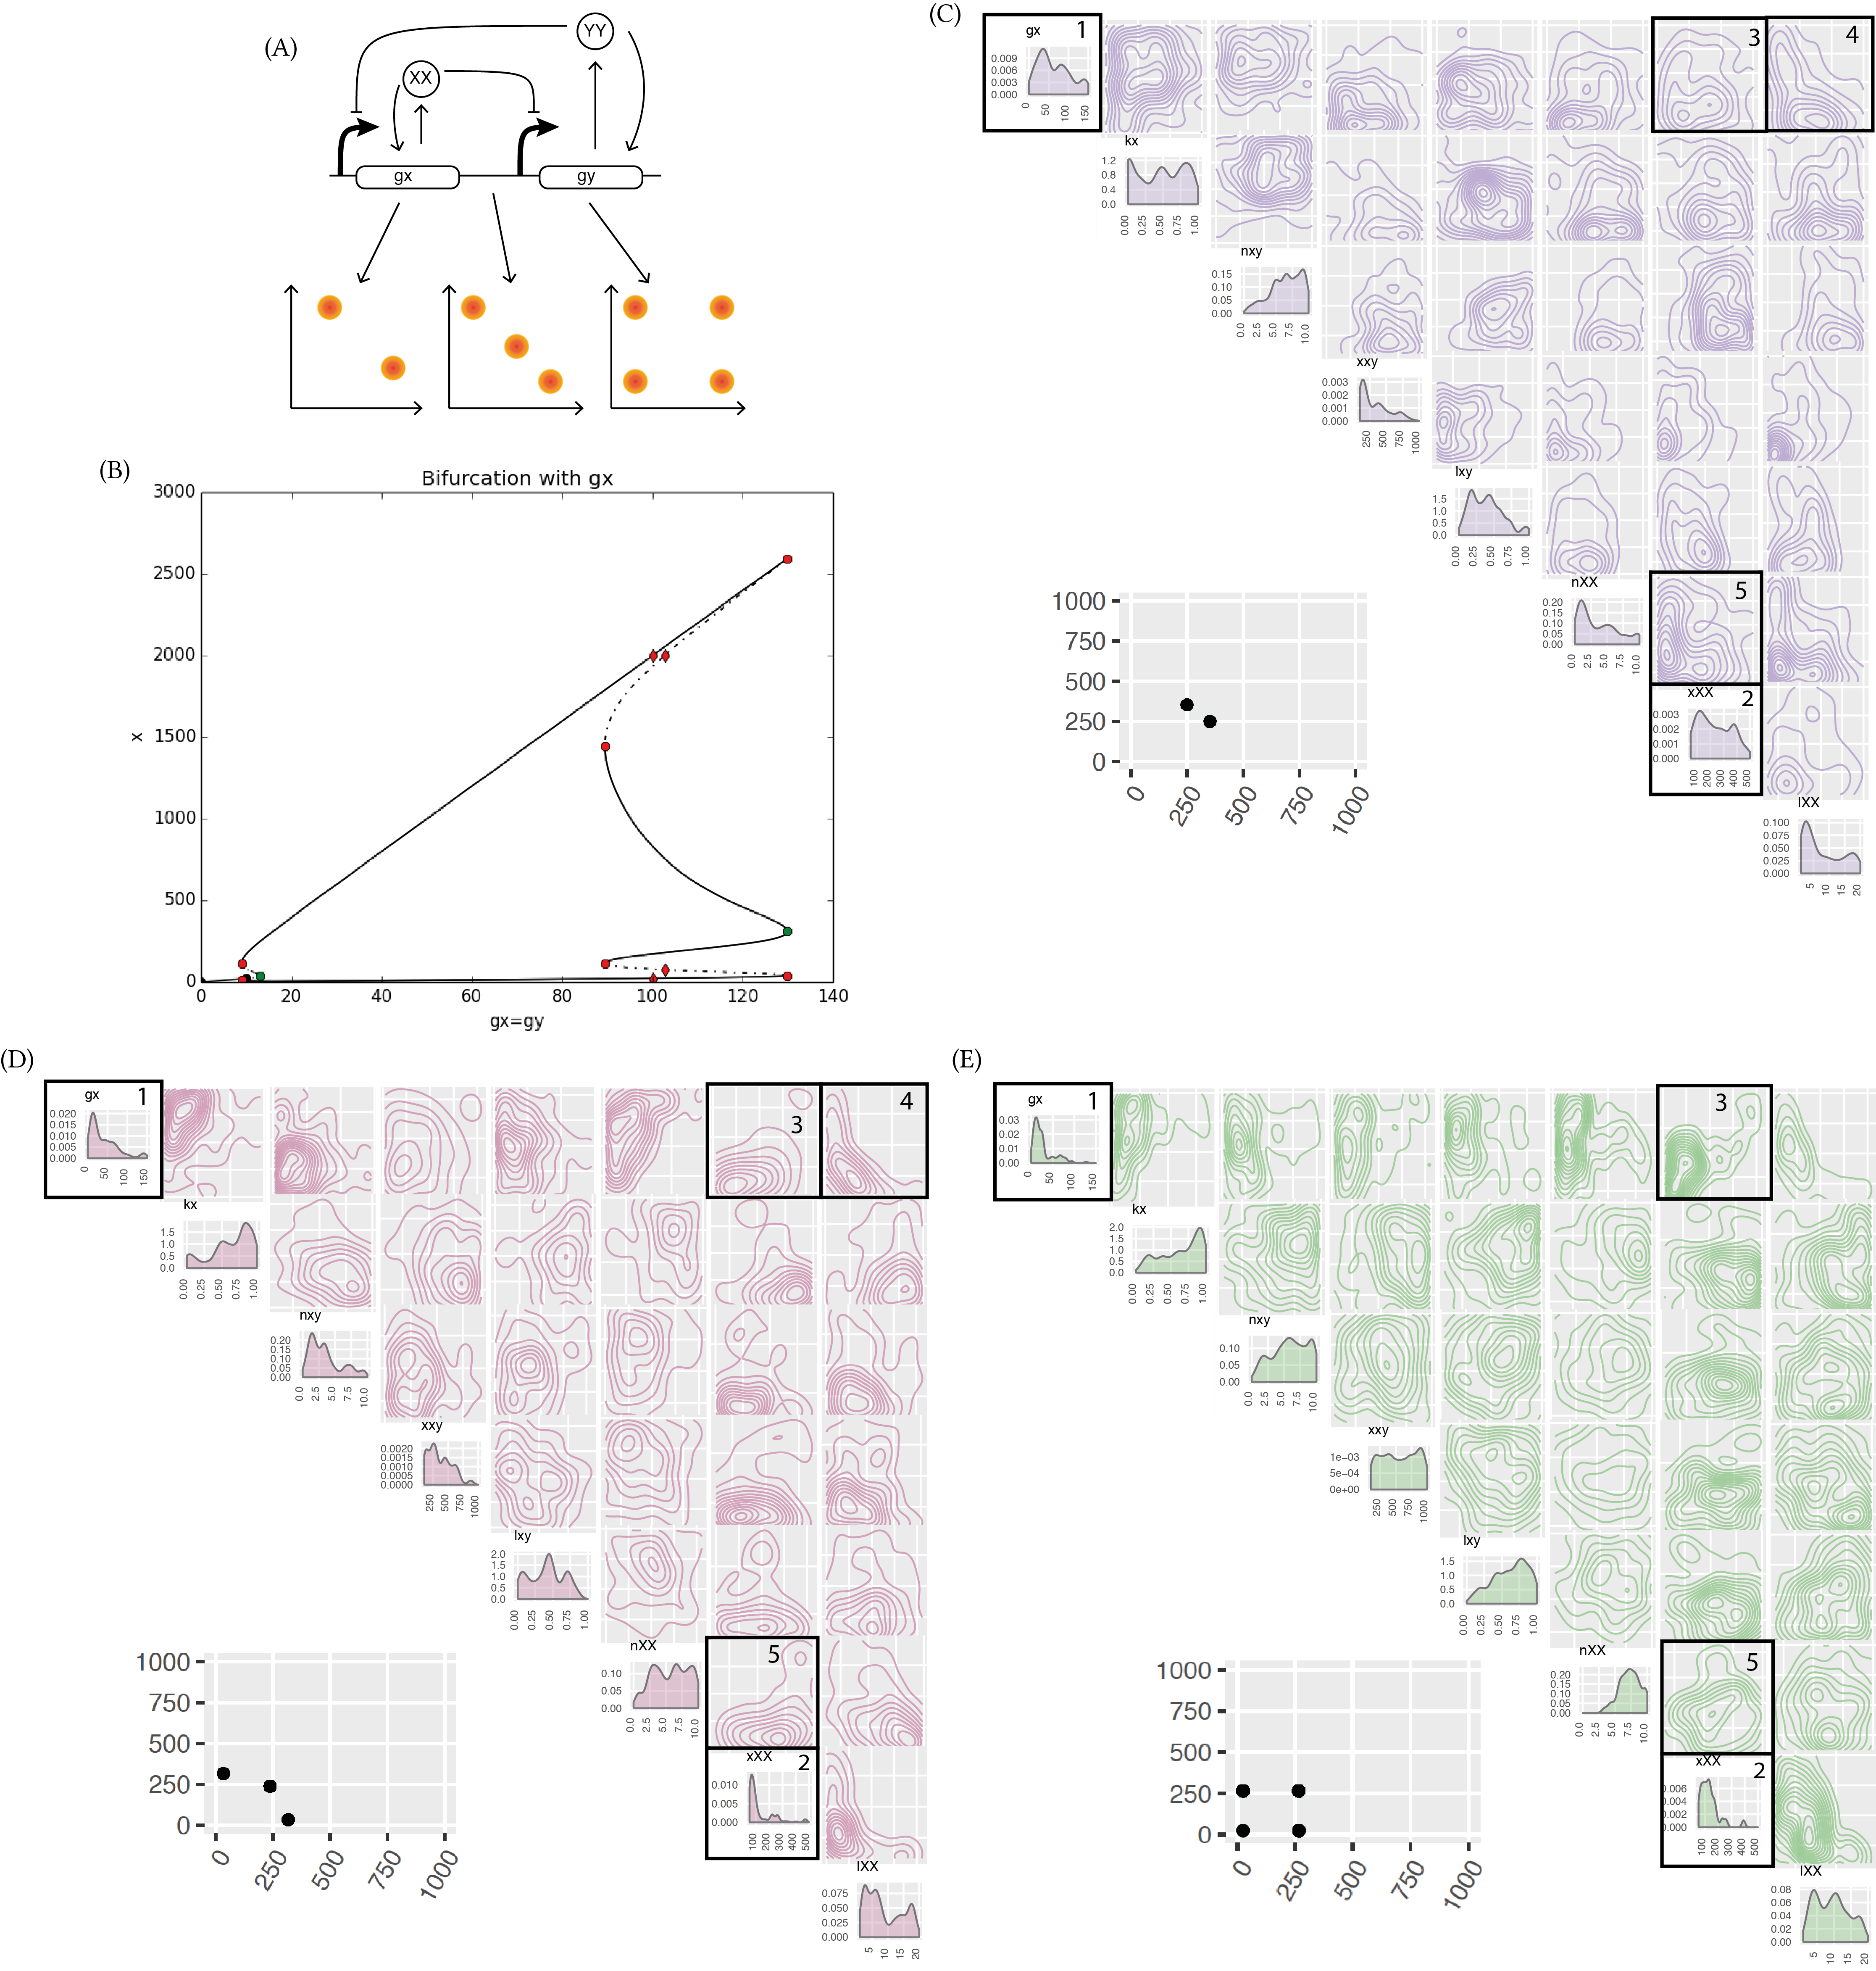
\includegraphics[width=1.2\textwidth]{../../chapters/chapterStabilityFinder/images/Lu_234.png}
		\caption[ Design principles of multistable switches]{ \label{fig:lu_234}: Design principles of multistable switches. (A) Using the Lu model with added positive autoregulation we uncover the design principles dictating if a switch will be bistable, tristable, or will have 4 steady states. (B-D) By considering the bivariate distributions of the parameters we can uncover the differences in the parameters of a bistable switch compared to a tristable switch, compared to a quadristable switch . The posterior distribution of the bistable switch is shown in purple, of the tristable switch in pink and of a quadristable in green. The bivariate distributions for which a difference is observed between the stabilities are in black boxes. An example of a phase plot from each behaviour is shown next to the corresponding posterior distribution.}
\end{figure*}



 Using StabilityFinder, the posterior distributions for bistable, tristable and quadristable behaviours in the \acrshort{dp-lu} model were obtained and then the posterior parameter distributions compared (Figure~\ref{fig:lu_234}). Upon examination of the posterior distributions for all three switches we observe that a subset of the posterior parameter values is different under the three behaviours. Differences are found in the univariate distribution of the parameters for gene expression, $gx$, as highlighted in Figure~\ref{fig:lu_234}, box 1. This parameter must be small for a quadristable switch to occur but there are no such restraints for a bistable or a tristable switch. Furthermore, parameter $xXX$ must be small for three and four steady states to be achieved but there are no such restraints for a bistable switch, as can be seen in Figure~\ref{fig:lu_234}, box 2. Parameter $xXX$ represents the Hill threshold concentration, and is equivalent to to the Hill constant described in Section~\ref{sec:hill}. This parameter dictates the substrate concentration at which the switch occurs. We find that the Hill constant has to be small in order to observe three or four steady states.

We also find a difference in the bivariate distributions in the posterior. Most notably, we find that parameters $xXX$ and $gX$ are tightly constrained in the tristable and the four steady state cases, where both parameters are required to be small, but less so in the bistable case (Figure~\ref{fig:lu_234}, box 3). Another notable difference is between parameters $xXX$ and $nXX$ shown in Figure~\ref{fig:lu_234}, box 5, where they are constrained in the tristable and quadristable cases but not the bistable case. There parameters represent the Hill constant and the Hill coefficient respectively. The Hill constant dictates the substrate concentration that results in half of the response, i.e. it is substrate concentration at which switching is observed. The Hill coefficient affects the steepness of the switching curve, as a higher Hill coefficient results in a steeper response, as illustrated in Figure~\ref{fig:hill_ex}.

Interestingly, we also find parameter correlations conserved between the three behaviours, as seen in Figure~\ref{fig:lu_234}, box 4, where parameters $lXX$ and $gx$, positive autoregulation and gene expression are negatively correlated in both cases.  This highlights the importance of treating unknown parameters as distributions rather than fixed values when studying the parameter values of a model, as they are capable of uncovering not only the ranges and values needed but also the correlations between parameters that would not have otherwise been detected. 






%Upon examination of the two dimensional marginal distributions we find that the correlation structure of a small subset of the posterior parameter values is in fact different under the two behaviours (Figure~\ref{fig:lu_234}). Most notably, we find differences in the bivariate distribution of the two parameters for gene expression, $gx$ and $gy$. In the tristable case the distribution is more constrained than in the bistable case, as both parameters must be small for tristability to arise. 


%Parameters $xYY$ and $gy$ are tightly constrained in the tristable case and both required to be small, but less so in the bistable case (Figure~\ref{fig:fig6}C, box 3). Another notable difference is between parameters $xXX$ and $lXX$ shown in Figure~\ref{fig:fig6}C, box 4, where they are constrained in the bistable case but not the tristable case. Interestingly, we also find parameter correlations conserved between the bistable and tristable case, as seen in Figure~\ref{fig:fig6}C, box 2, where parameters $lXX$ and $gx$, positive autoregulation and gene expression are negatively correlated in both cases.  This highlights the importance of treating unknown parameters as distributions rather than fixed values when studying the parameter values of a model, as they are capable of uncovering not only the ranges and values needed but also the correlations between parameters that would not have otherwise been detected.

I further analyse these models by studying the phase plots resulting from simulating the particles from the posterior distribution to steady state. The phase plots from 100 particles from each posterior are shown in Figure~\ref{fig:lu_234_phase}. We find that there is a strong conservation on the locations of the steady states between each particle. This indicates that the steady states in a two-node toggle switch tend to be symmetrical. This gives rise to the patterns seen in Figure~\ref{fig:lu_234_phase}. It is important to highlight that this was not set as a requirement for the behaviour of the switch in StabilityFinder, but the behaviour that these models gave rise to. There were no constraints on the level or location of the steady states. 

The symmetrical steady states are especially evident in the quadristable switch.  For every steady state at (0,0) there is another steady state on its diagonal, at $XX$ = $YY$. All the combinations of these two steady states form the straight line seen in Figure~\ref{fig:lu_234_phase}C. This indicates that two of the four steady states exist where $XX$ = $YY$. The other two exist where one of the two proteins dominates the other.  There are four distinct states of the system: both proteins high, both low, XX high/YY low and XX low/YY high. 


This same principle can be seen in the bistable and the tristable switches. In the bistable switch the two steady states are also symmetrical and one never completely dominates the other. For the tristable case we observe that two of the steady states exist where the levels of one protein is much larger than the other, and a third steady state exists where $XX$ = $YY$. This finding can be exploited in a synthetic biology application. Building a switch whose states are always symmetrical makes it easy to distinguish which state the system is in. By measuring one of the proteins in the system it can be inferred what the levels of the other are. 

We also observe that the third steady state is not necessarily a 'dead' state, but they can exist over a range of values for $XX$ and $YY$.

\begin{figure*}[bp]
	\begin{center}
		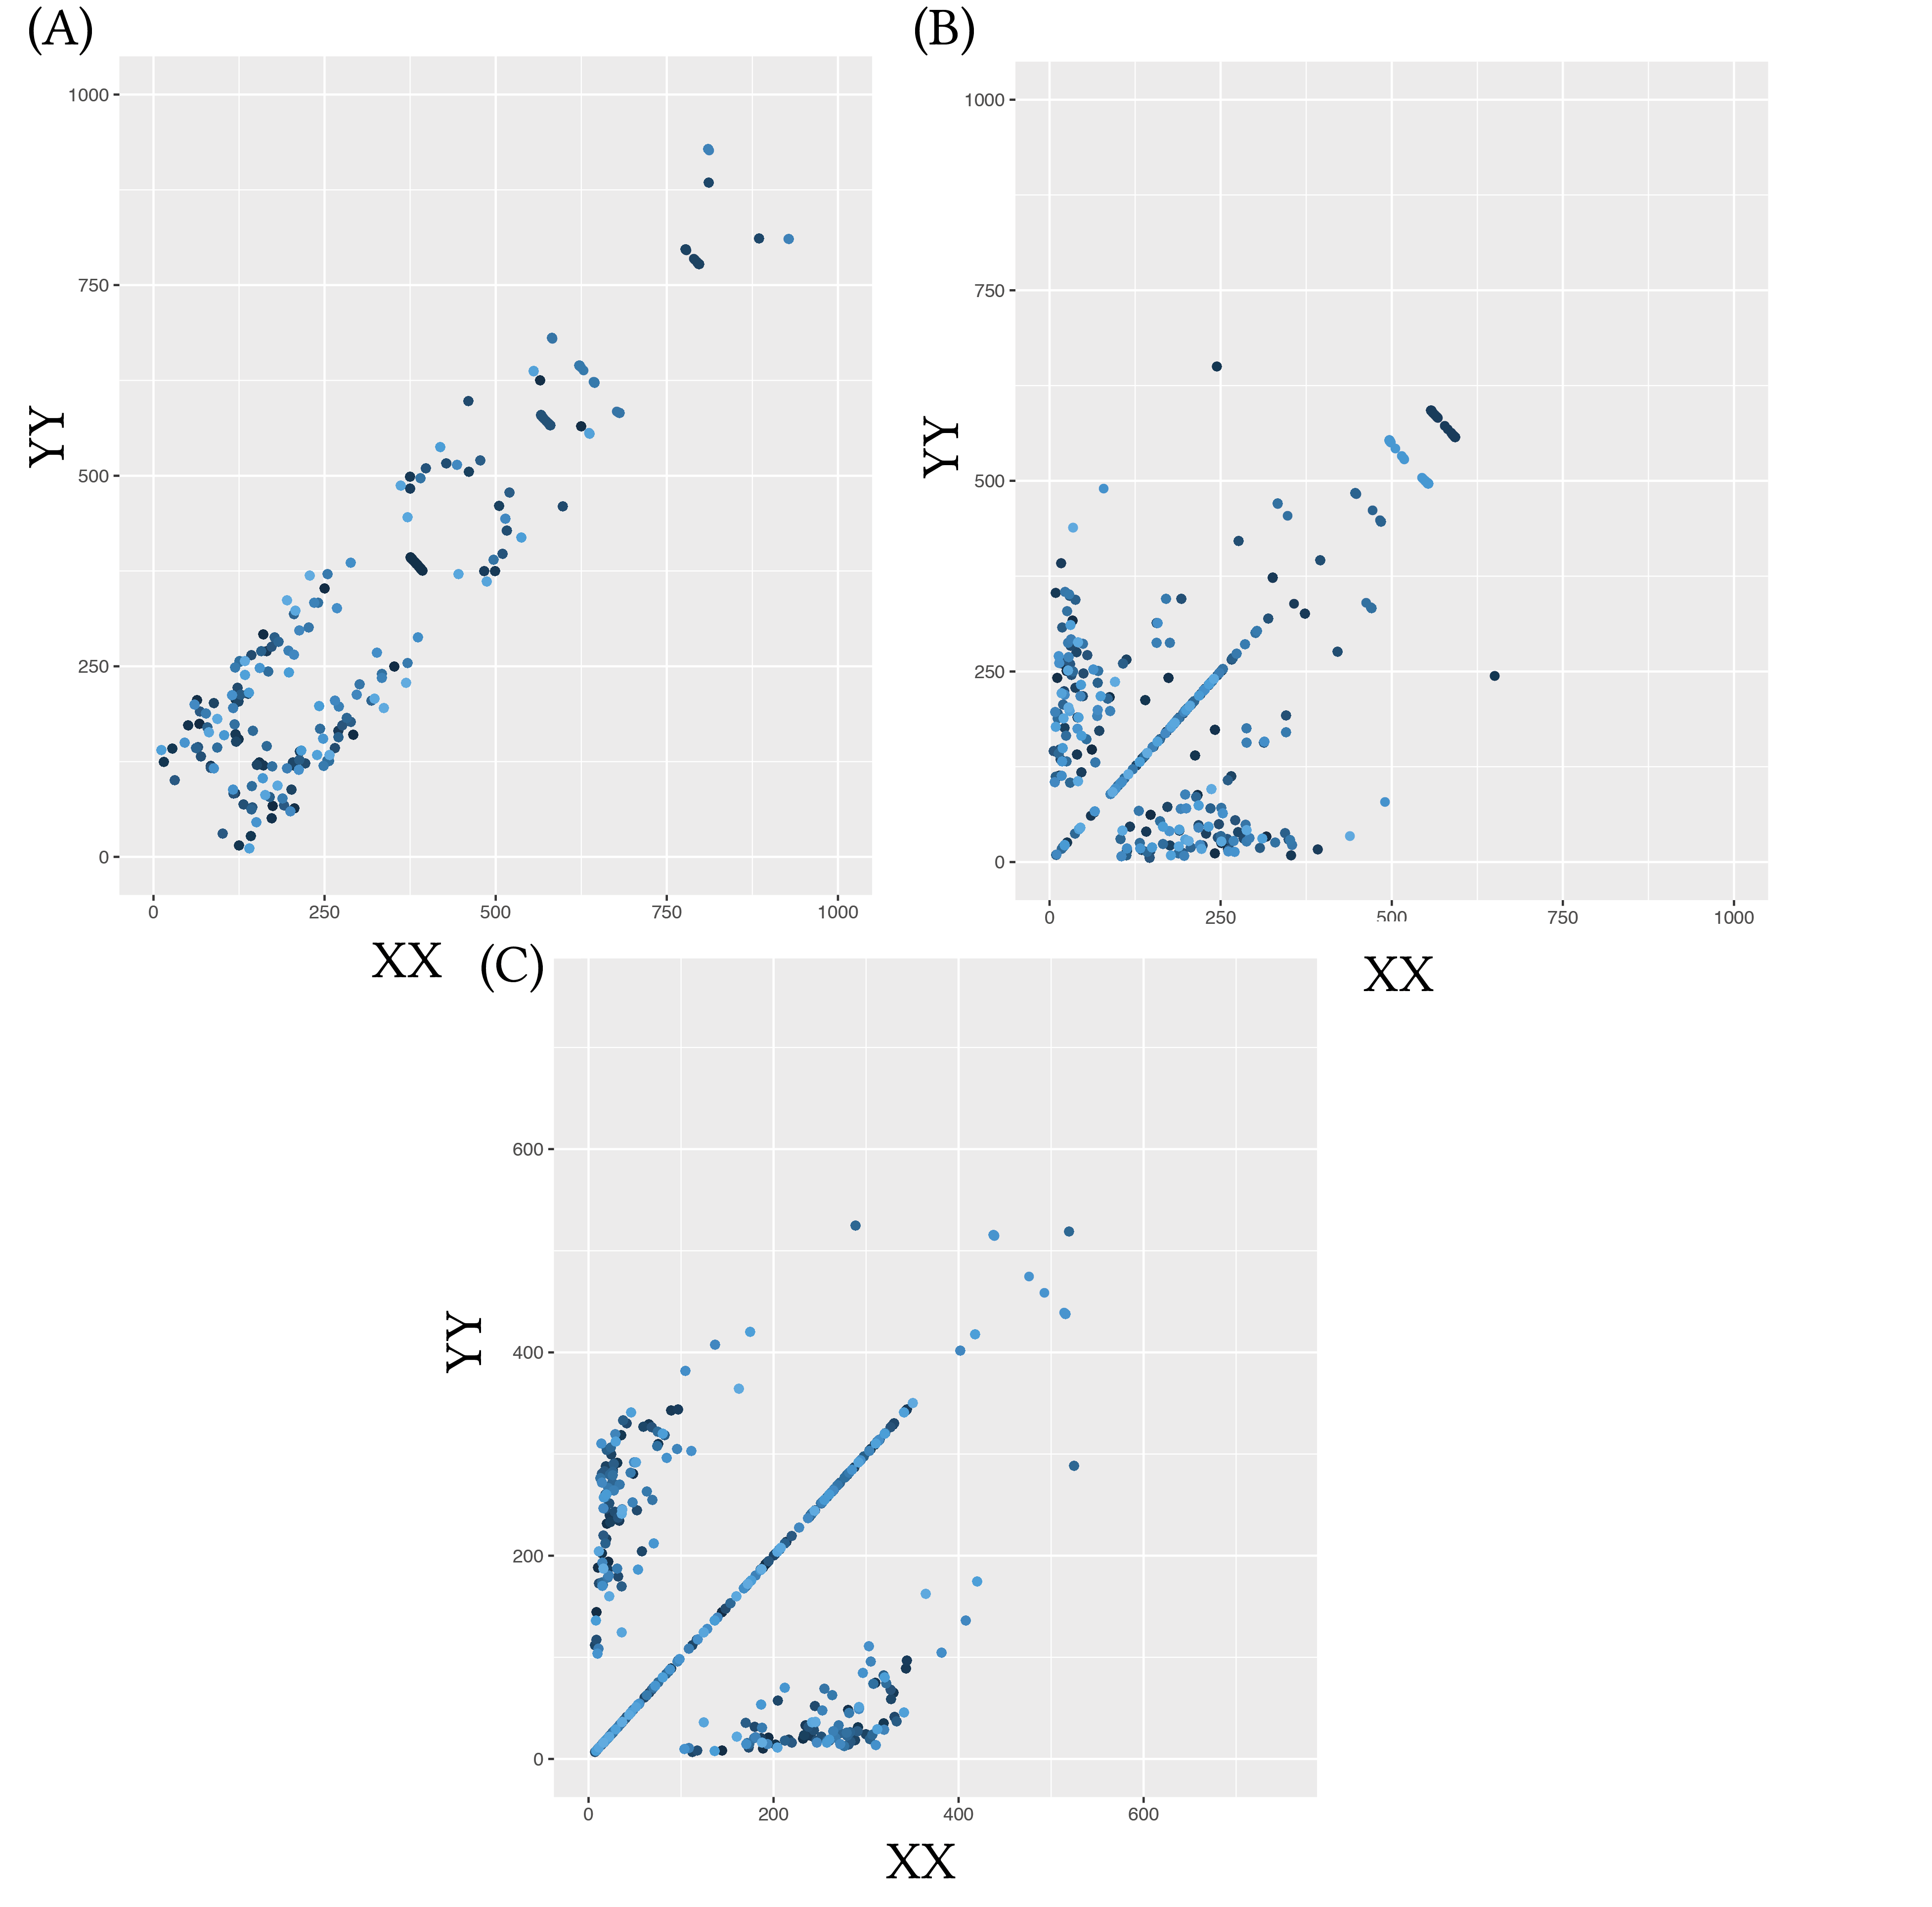
\includegraphics[width=\textwidth]{../../chapters/chapterStabilityFinder/images/LU-234-phase-all.png}
		\caption[Phase plots of multistable switches]{ \label{fig:lu_234_phase}: The phase plots from 100 particles from each posterior. (A) The \\acrshort{cs-lu} (B) \acrshort{sp-lu} and (C) \acrshort{dp-lu}. Each particle is represented by a different shade of blue. We find a strong conservation on the location of the steady states between particles.  }
	\end{center}
\end{figure*}

%\begin{figure*}[h]
%\begin{center}
%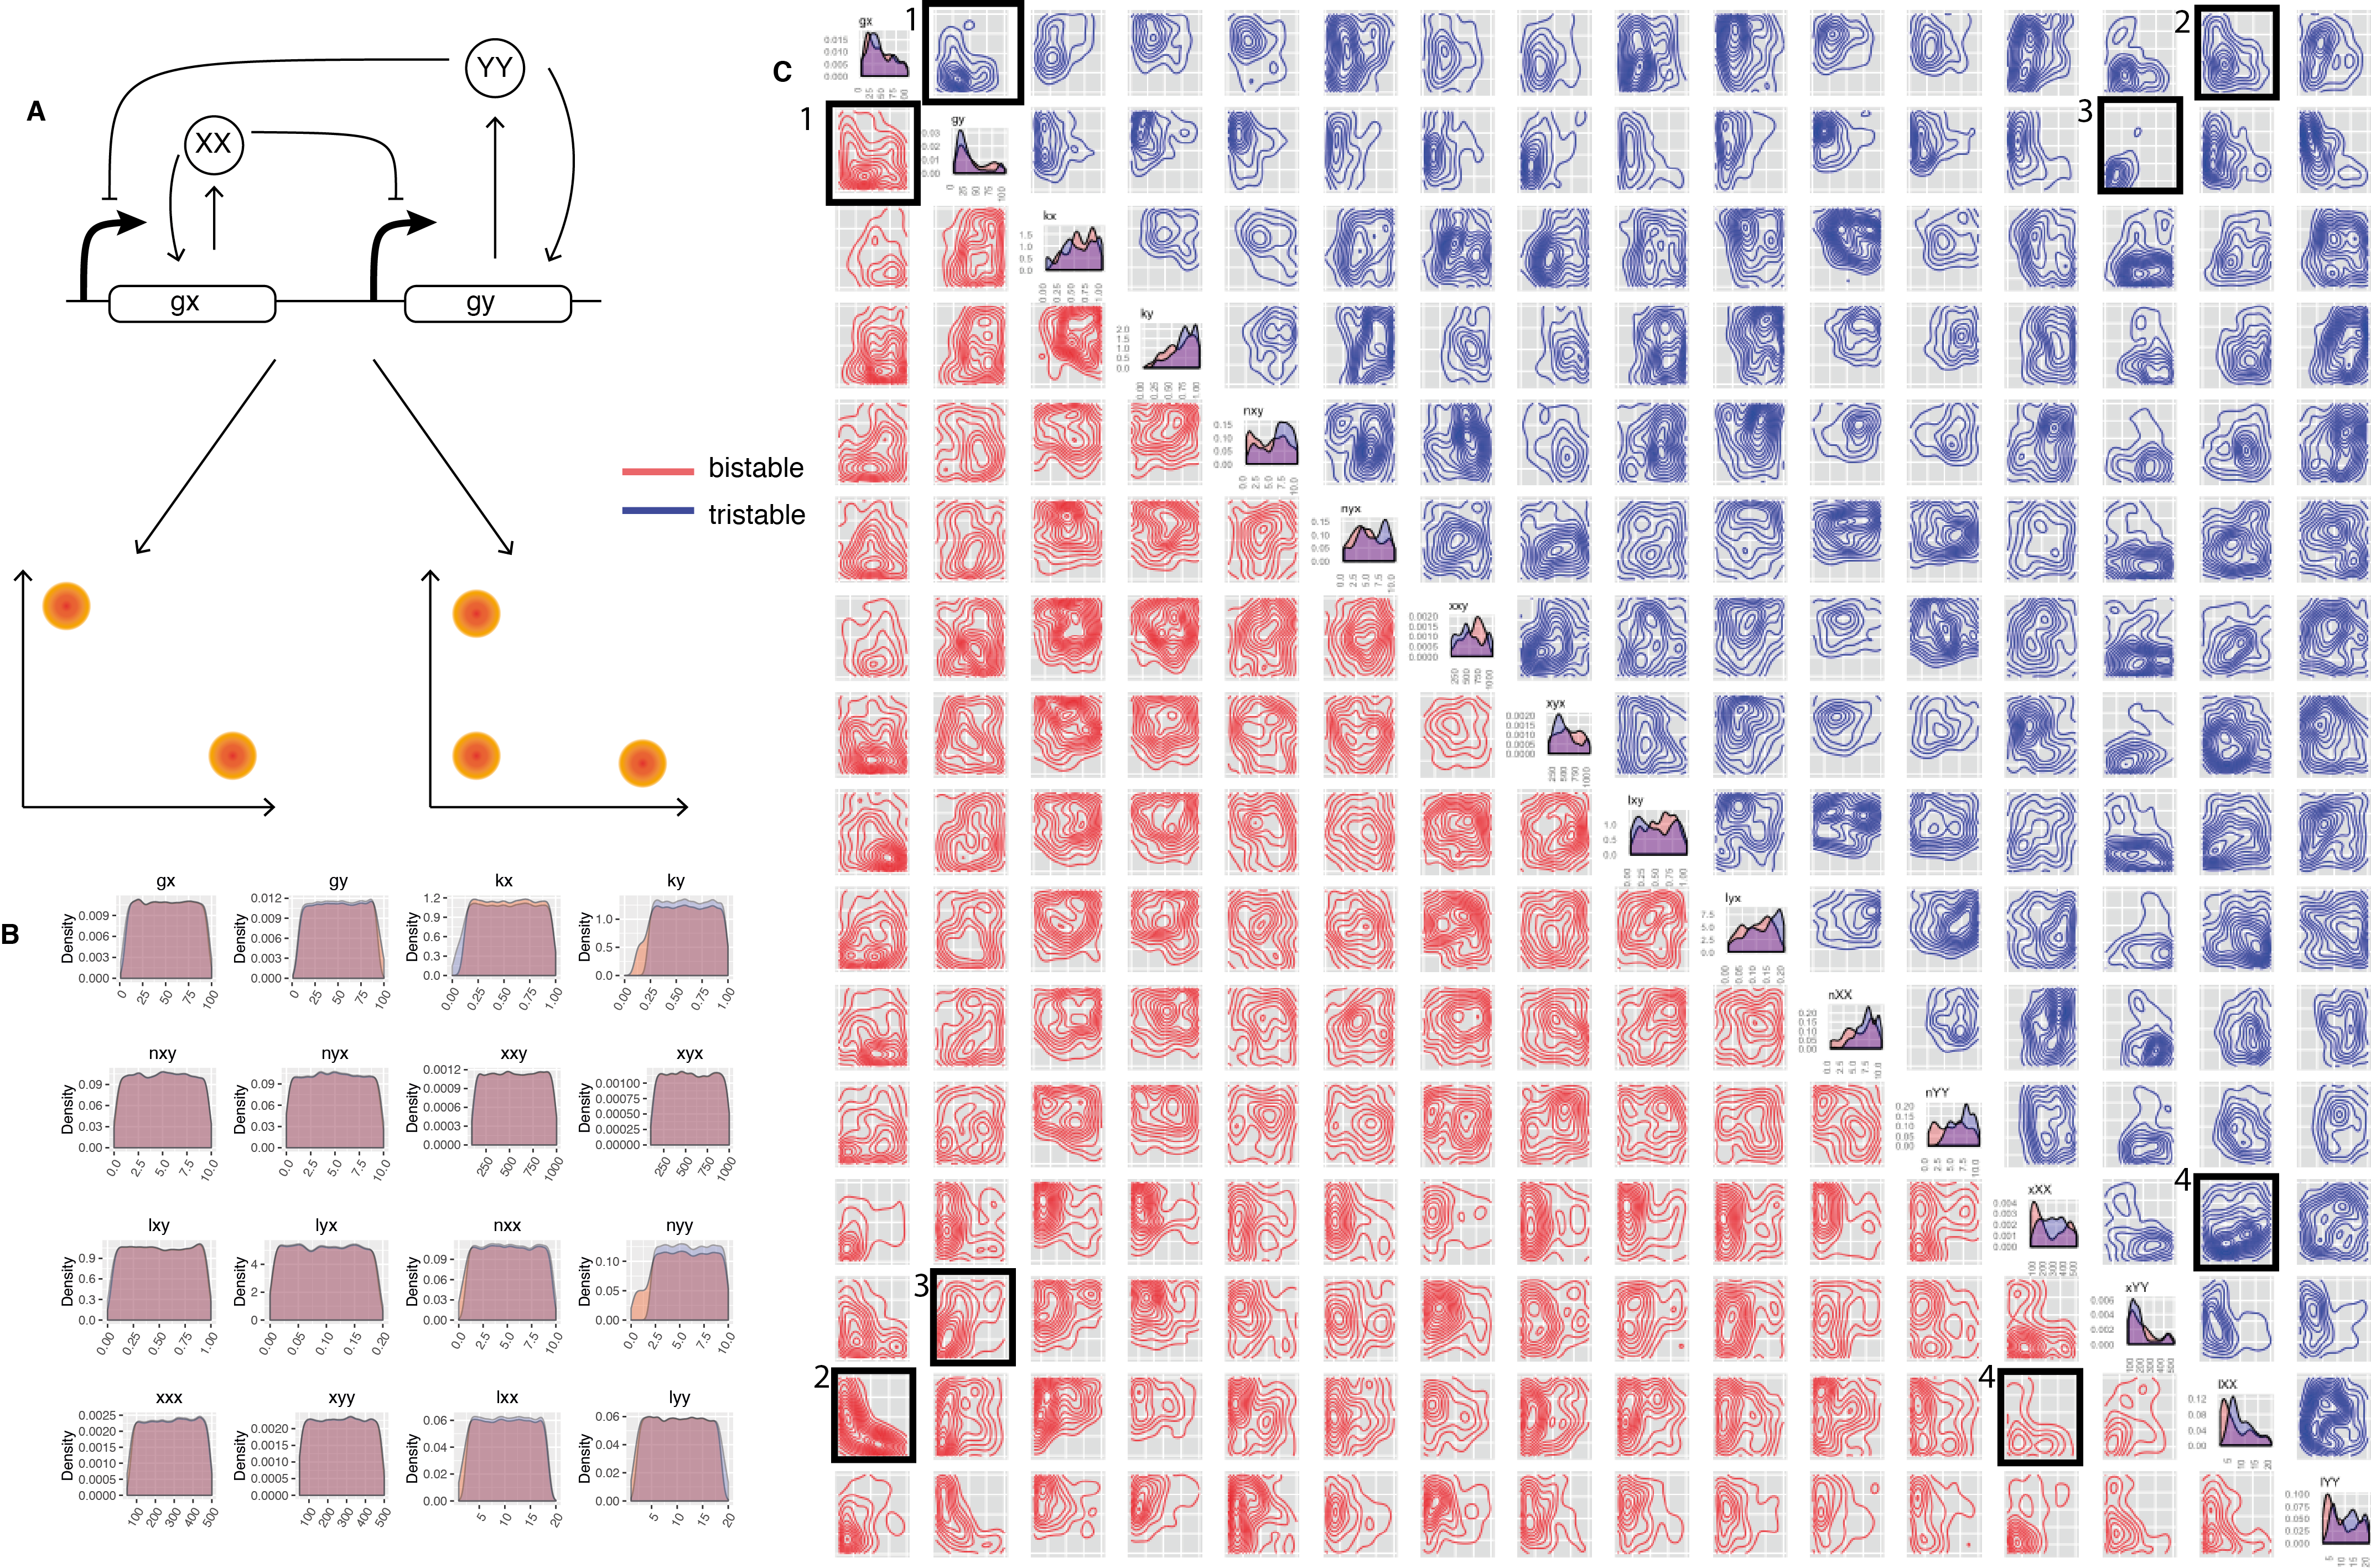
\includegraphics[width=\textwidth]{../../chapters/chapterStabilityFinder/images/Lu_bi_tri_design_princ.png}
%\caption[LoF caption]{ \label{fig:fig6}: Design principles of a tristable switch. (A) Using the Lu model with added positive autoregulation we uncover the design principles dictating if a switch will be bistable or tristable. (B) By considering each parameter separately we cannot find a significant difference in the parameter values acceptable for a bistable versus a tristable switch. (C) By considering the bivariate distributions of the parameters we can uncover the differences in the parameters of a bistable switch compared to a tristable switch. The posterior distribution of the bistable switch is shown in red and of the tristable switch in blue. The bivariate distributions for which a difference is observed between a bistable and a tristable switch are in black boxes. }
%\end{center}
%\end{figure*}


\clearpage
\subsubsection{Extending the Lu switch to three nodes}
To further demonstrate the flexibility of StabilityFinder I investigated a system capable of higher stabilities. Multistability is found in differentiating pathways, like the myeloid differentiation pathway~\autocite{Ghaffarizadeh:2014bt, Cinquin:2005go}. I allow for these more complex dynamics by extending the \acrshort{dp-lu} model by adding another gene, making it a three gene switch.  This new system is depicted in Figure~\ref{fig:fig8}A. This model has symmetric parameters, which means that the parameters for equivalent reactions (e.g. gene expression) are the same. In StabilityFinder I look for six steady states, the output being in nodes $X$ and $Y$ and using the priors shown in Table~\ref{tab:multi_priors}. We successfully find that the system is capable of six steady states, as shown in Figure~\ref{fig:fig8}C. 

\begin{table}[htpb]
\centering
\caption{Priors used in the three-node switch}
\label{tab:multi_priors}
\begin{tabular}{@{}lll@{}}
\toprule
Parameter                           & Symbol & Range (nM/min)  \\ \midrule
Production rate (Proteins/Minute)               & gx        & 3-5    \\
Degradation rate  (Minute\textsubscript{-1})             & kx        & 0-0.2     \\
Hill coefficient               & nxy       & 0-2    \\
Hill thresholds concentration (Proteins) & xxy       & 140-160 \\
Transcription rate fold change & lxy       & 0-0.2     \\
Hill coefficient               & nxx       & 2-4     \\
Hill thresholds concentration (Proteins) & xxx       & 90-110  \\
Transcription rate fold change & lxx       & 8-12    \\ \bottomrule
\end{tabular}
\end{table}

\begin{figure*}[h]
\begin{center}
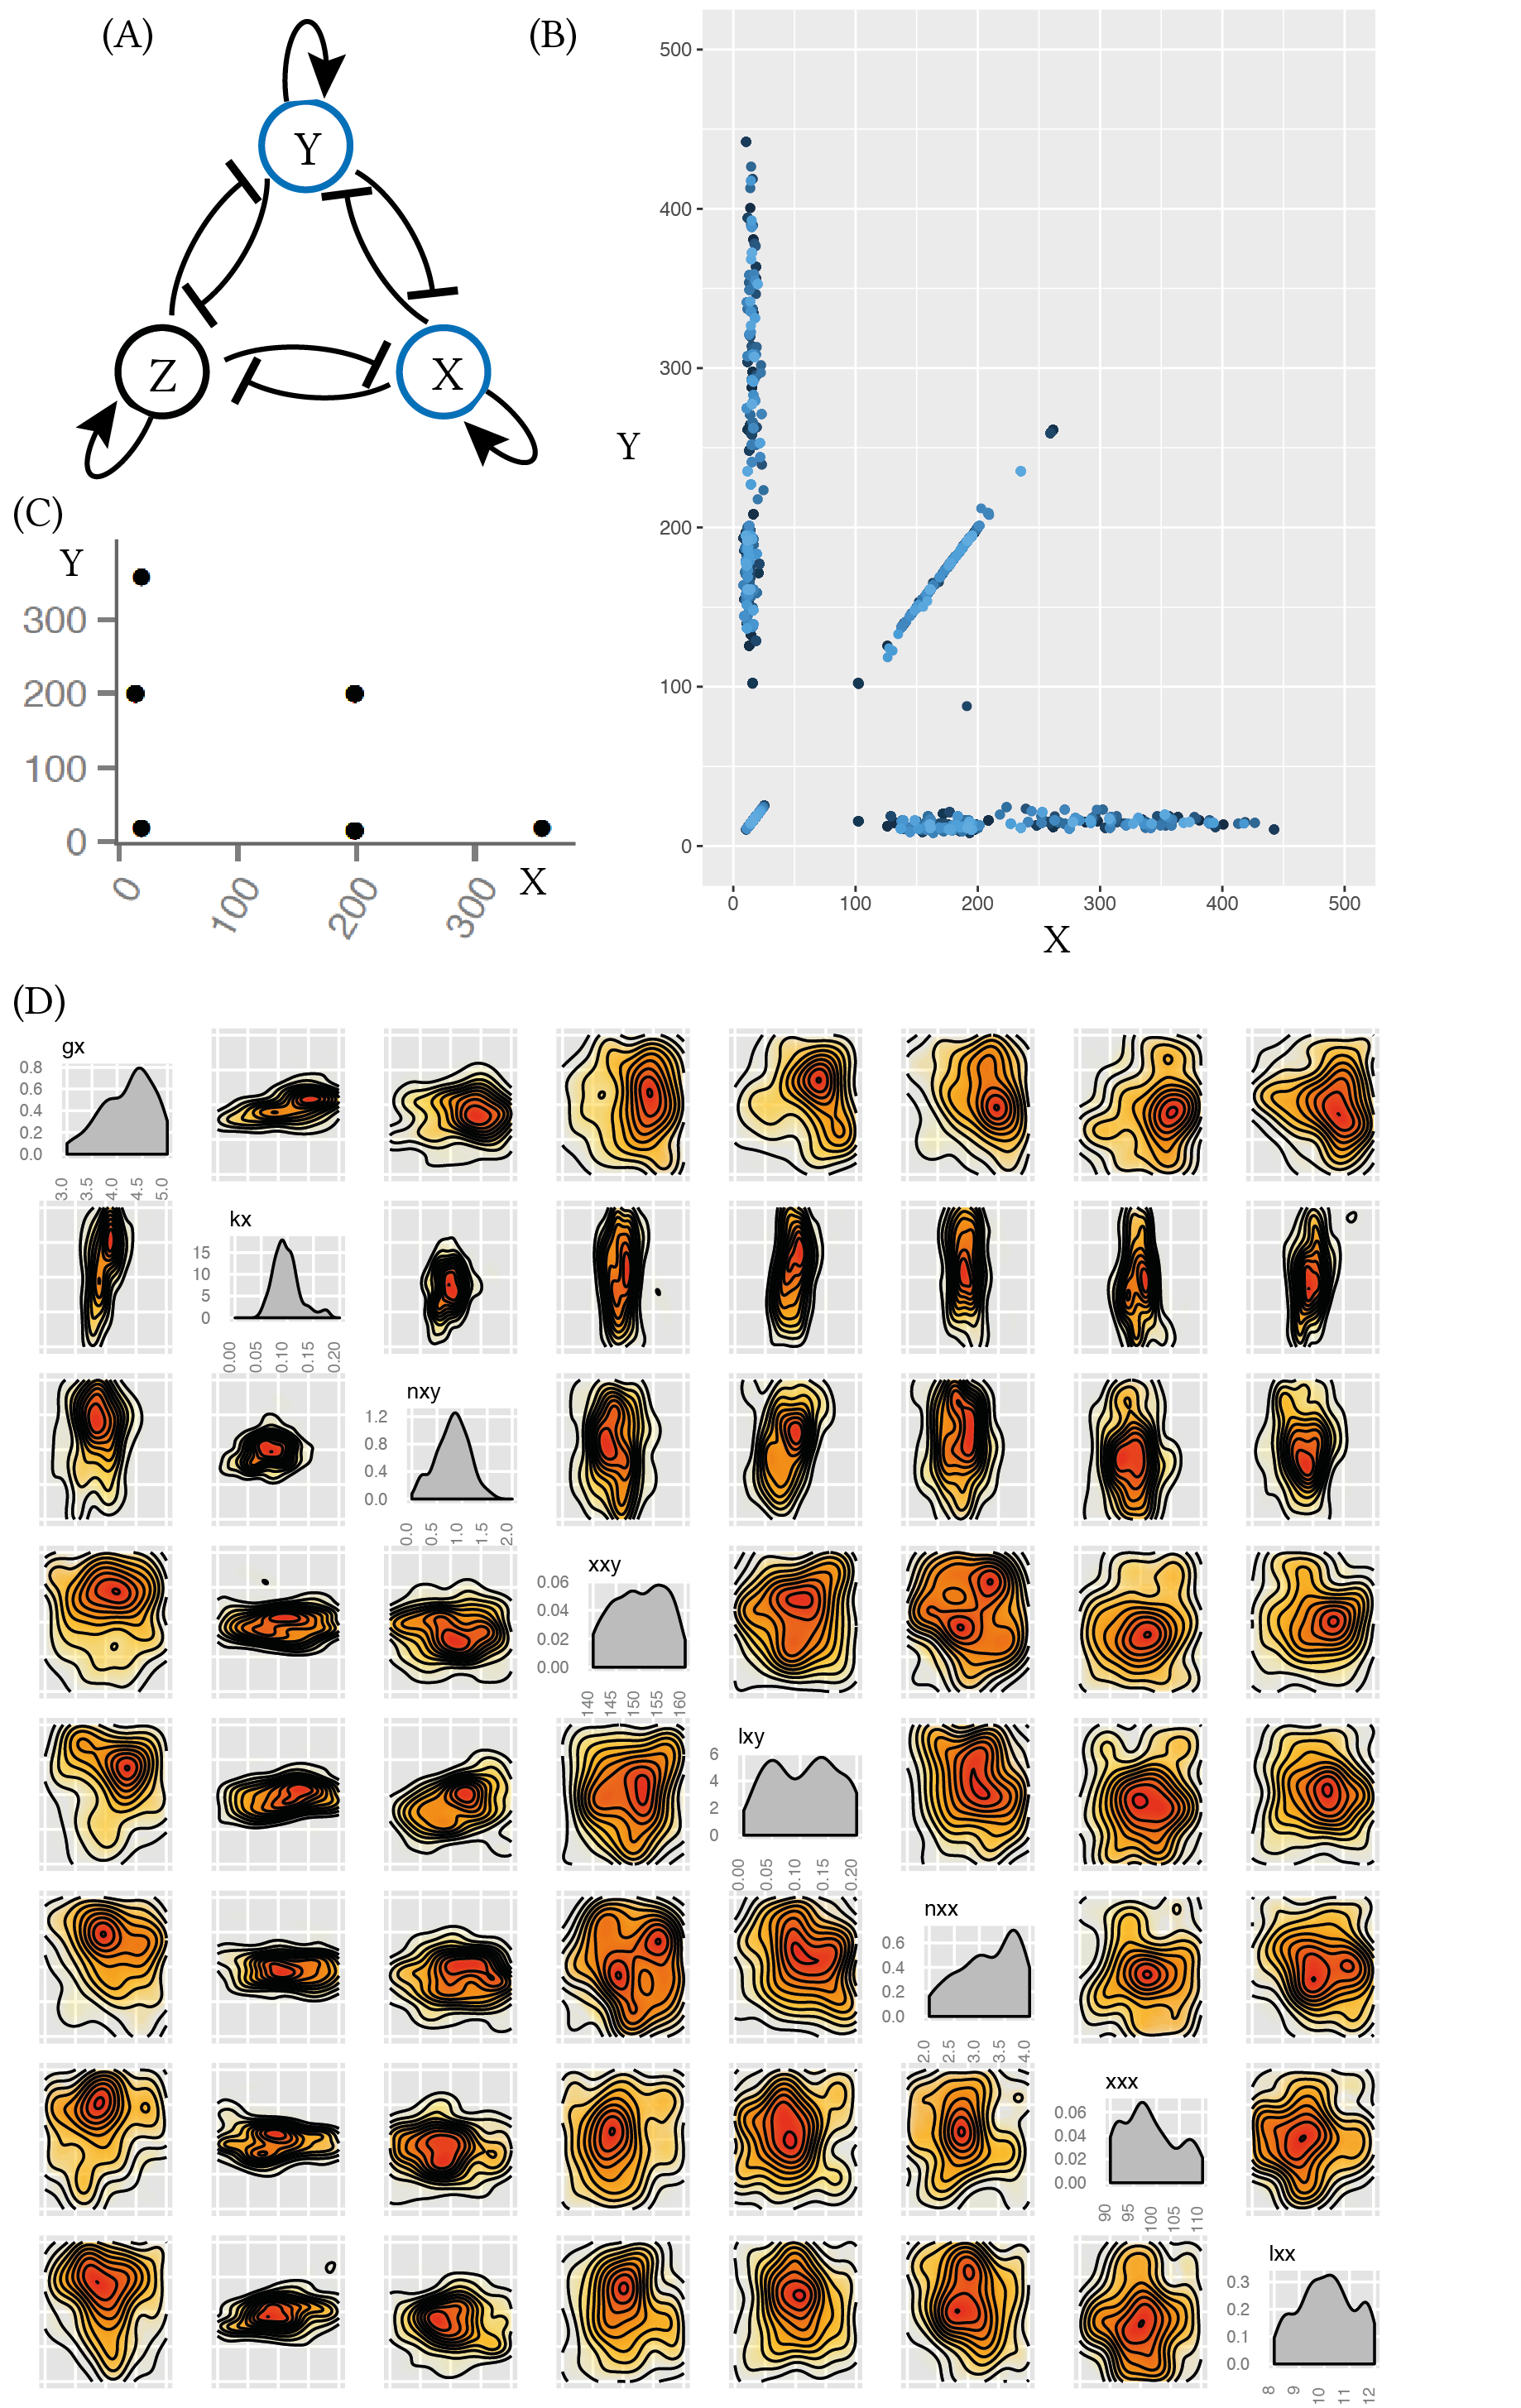
\includegraphics[scale=0.6]{../../chapters/chapterStabilityFinder/images/lu_6ss.png}
\caption[The three-node mutual repression model, with added positive auto-regulation on each node.]{ \label{fig:fig8}: The three-node mutual repression model, with added positive auto-regulation on each node. (A) The model. The model is studied in two dimensions using StabilityFinder, for nodes $X$ and $Y$. (B) The phase plot of 100 particles from the posterior found by StabilityFinder. There are 6 steady states. (C) The posterior distribution of the 6-steady state three-node system. Parameters $kx$ and $nxy$ are the most constrained.}
\end{center}
\end{figure*}


We find that the most constrained parameters for this behaviour are again the degradation rate of the proteins, $kx$. If they are too large or too small the system will not exhibit hexa-stability. Additionally we find that the Hill coefficients for the repressors, $nxy$, are constrained to be smaller than 1.5 as seen in Figure~\ref{fig:fig8}D. 

Consistently with the results found in section~\ref{sec:lu_234}, we find that the steady states are symmetric (Figure~\ref{fig:fig8}B). Each of six steady states exists in symmetry with another one, in tightly constrained regions. This example demonstrates that StabilityFinder can be used to elucidate the dynamics of more complex network architectures, which will be key to the successful design and construction of novel gene networks as synthetic biology advances.


\clearpage
\subsection{StabilityFinder used on the more general mass action switches}
\label{sec:ma_sw}						
%Although the DP switch can achieve tristability, we investigated how the addition of positive autoregulation alters the robustness of the switch for bistable behaviour. Here we define a robust system as a device that can withstand fluctuations in parameter values and still produce the desired behaviour (parametric robustness). Feedback loops are well known key regulatory motifs~\autocite{Brandman:2005ci}. Although negative feedback loops are essential for homeostasis and buffering~\autocite{Thomas:1995id} and can increase robustness to extrinsic noise sources, we focussed on the addition of positive feedback because this has been shown to increase robustness in other systems \autocite{XXX}. We use StabilityFinder to compare the two models, and determine whether its worthwhile building a bistable circuit with added positive feedback.
%StabilityFinder allows us to study more complex systems and to take stochasticity into account. This is relevant in a biological systems in which realistic models tend to involve many species and interactions and where small molecule numbers and external noise are non negligible. 

In order to study the switch system in a more realistic way, I developed an extension to the switches used in Sections~\ref{sec:gard} and~\ref{sec:lu}. This new set of switches does not use the \acrfull{qssa} that is often used in modelling the toggle switch. Using mass action, this changes the two-equation system used in~\textcite{Gardner:2000vha} and~\textcite{Lu:2014kc} into a system of 8 \acrshort{ode}s and 10 parameters in the classical switch case with no autoregulation (model \acrshort{cs-ma}). The equations describing the system are shown below. 
$$
\begin{array}{cccc}
      \textrm{gA}\stackrel{\textrm{geA}}{\longrightarrow}\textrm{gA} + \textrm{A} \\
      \textrm{gB}\stackrel{\textrm{geB}}{\longrightarrow}\textrm{gB} + \textrm{B} \\
      \textrm{A} + \textrm{A} \stackrel{\textrm{dim}}{\longrightarrow}\textrm{A2} \\
      \textrm{A2} \stackrel{\textrm{dim r}}{\longrightarrow}\textrm{A} + \textrm{A} \\
      \textrm{B} + \textrm{B} \stackrel{\textrm{dim}}{\longrightarrow} \textrm{B2} \\
      \textrm{B2} \stackrel{\textrm{dim\_r}}{\longrightarrow}\textrm{B} + \textrm{B} \\
      \textrm{gA} + \textrm{B2} \stackrel{\textrm{repA}}{\longrightarrow}\textrm{B2gA} \\
      \textrm{B2gA} \stackrel{\textrm{rep\_r}}{\longrightarrow}\textrm{B} + \textrm{gA} \\
      \textrm{gB} + \textrm{A2} \stackrel{\textrm{repB}}{\longrightarrow}\textrm{A2gB} \\
      \textrm{A2gB} \stackrel{\textrm{rep\_r}}{\longrightarrow}\textrm{A2} + \textrm{gB} \\
      \textrm{A} \stackrel{\textrm{deg}}{\longrightarrow}\textrm{\O}\\
      \textrm{A2} \stackrel{\textrm{deg\_dim}}{\longrightarrow} \varnothing\\
      \textrm{B2} \stackrel{\textrm{deg\_dim}}{\longrightarrow}\varnothing\\
\end{array}
$$

For the model with added double positive autoregulation (model \acrshort{dp-ma}) the following equations are added to the system: 

$$
\begin{array}{cccc} 
    \textrm{A2} + \textrm{gA} \stackrel{\textrm{aut 1}}{\longrightarrow} \textrm{A2gA} \\
    \textrm{A2gA} \stackrel{\textrm{aut 2}}{\longrightarrow} \textrm{A} + \textrm{A2gA}\\
    \textrm{A2gA} \stackrel{\textrm{aut 3}}{\longrightarrow} \textrm{A2}+ \textrm{gA}  \\
    \textrm{B2} + \textrm{gB} \stackrel{\textrm{aut 1}}{\longrightarrow} \textrm{B2gB} \\
    \textrm{B2gB} \stackrel{\textrm{aut 2}}{\longrightarrow} \textrm{B} + \textrm{B2gB}\\
    \textrm{B2gB} \stackrel{\textrm{aut 3}}{\longrightarrow} \textrm{B2}+ \textrm{gB}  \\
\end{array}
$$

The \acrshort{ode}s describing the above switches are shown in Appendix~\ref{ap:ODEs}. These models are too complex to be solved analytically and I use StabilityFinder to fit the models to a bistable behaviour. The two models used and the resulting phase plots are shown in Figure~\ref{fig:ma-cs-dp-phase} and the posterior distributions  obtained are shown in Figure~\ref{fig:ma-sym-det-post}. 

\begin{figure*}[htbp]
\begin{center}
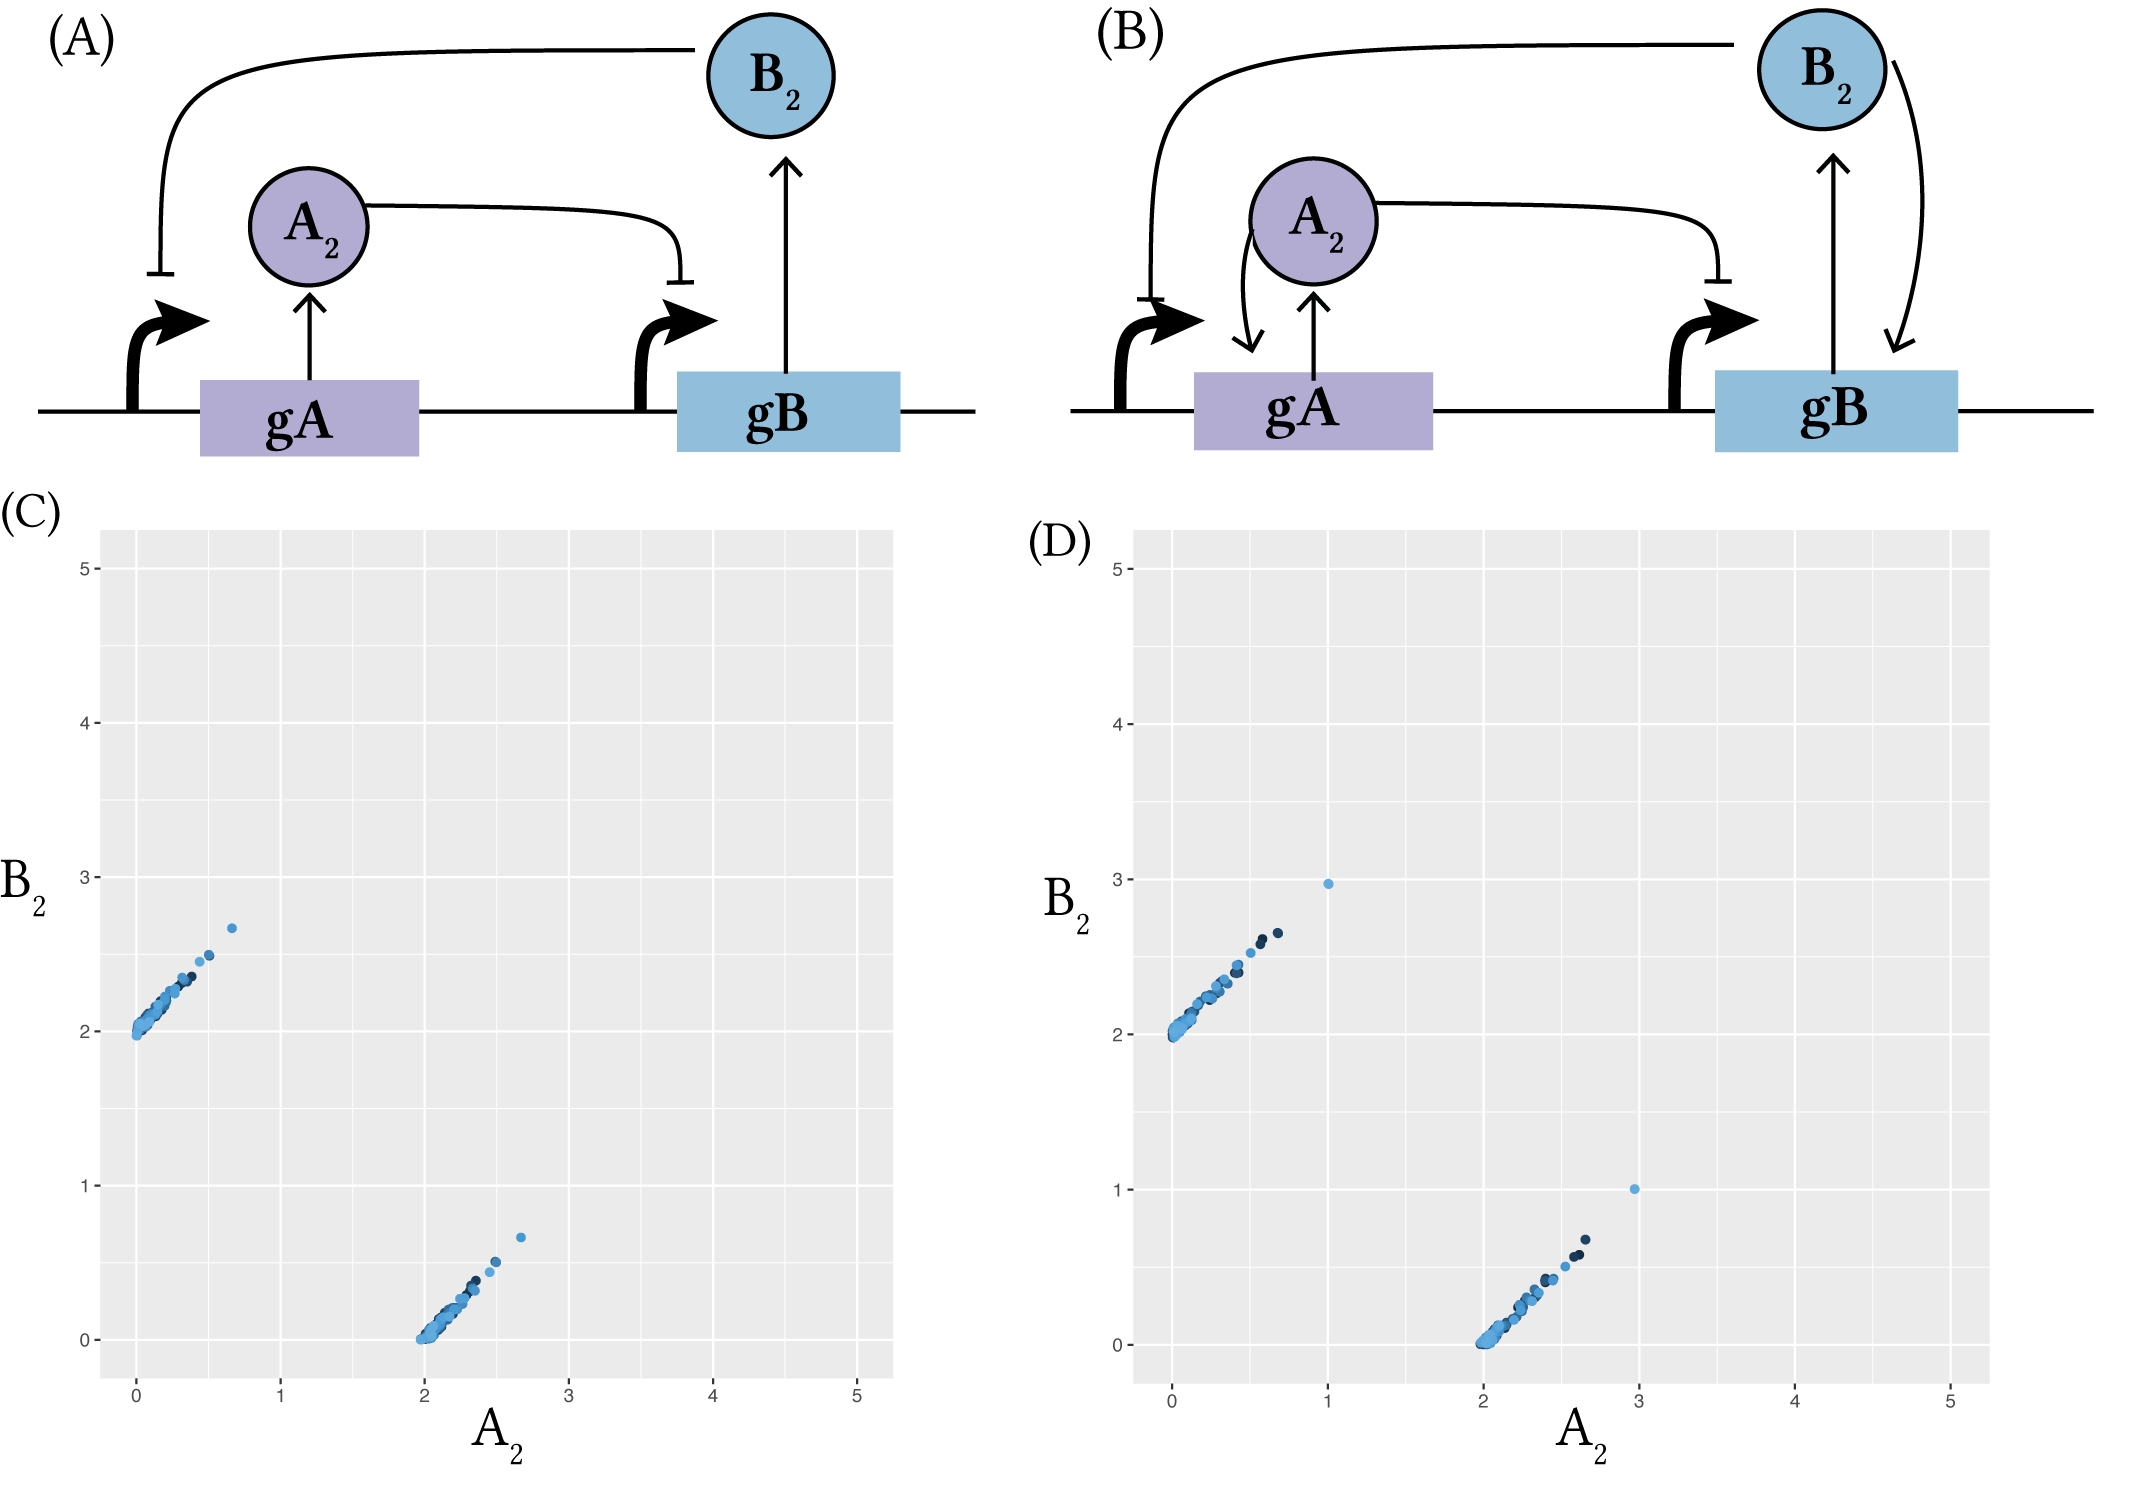
\includegraphics[scale=0.7]{../../chapters/chapterStabilityFinder/images/MA-cs-dp-phase.png}
\caption[The mass action togge switches and phase plots]{ \label{fig:ma-cs-dp-phase}: The two mass action switches I developed. (A) The simple switch \acrshort{cs-ma} (B) The switch with double positive autoregulation \acrshort{dp-ma}. (C, D) The phase plots of 100 particles simulated from the posterior distributions of the bistable mass action switches.}
\end{center}
\end{figure*}


\begin{figure*}[htbp]
\centerfloat
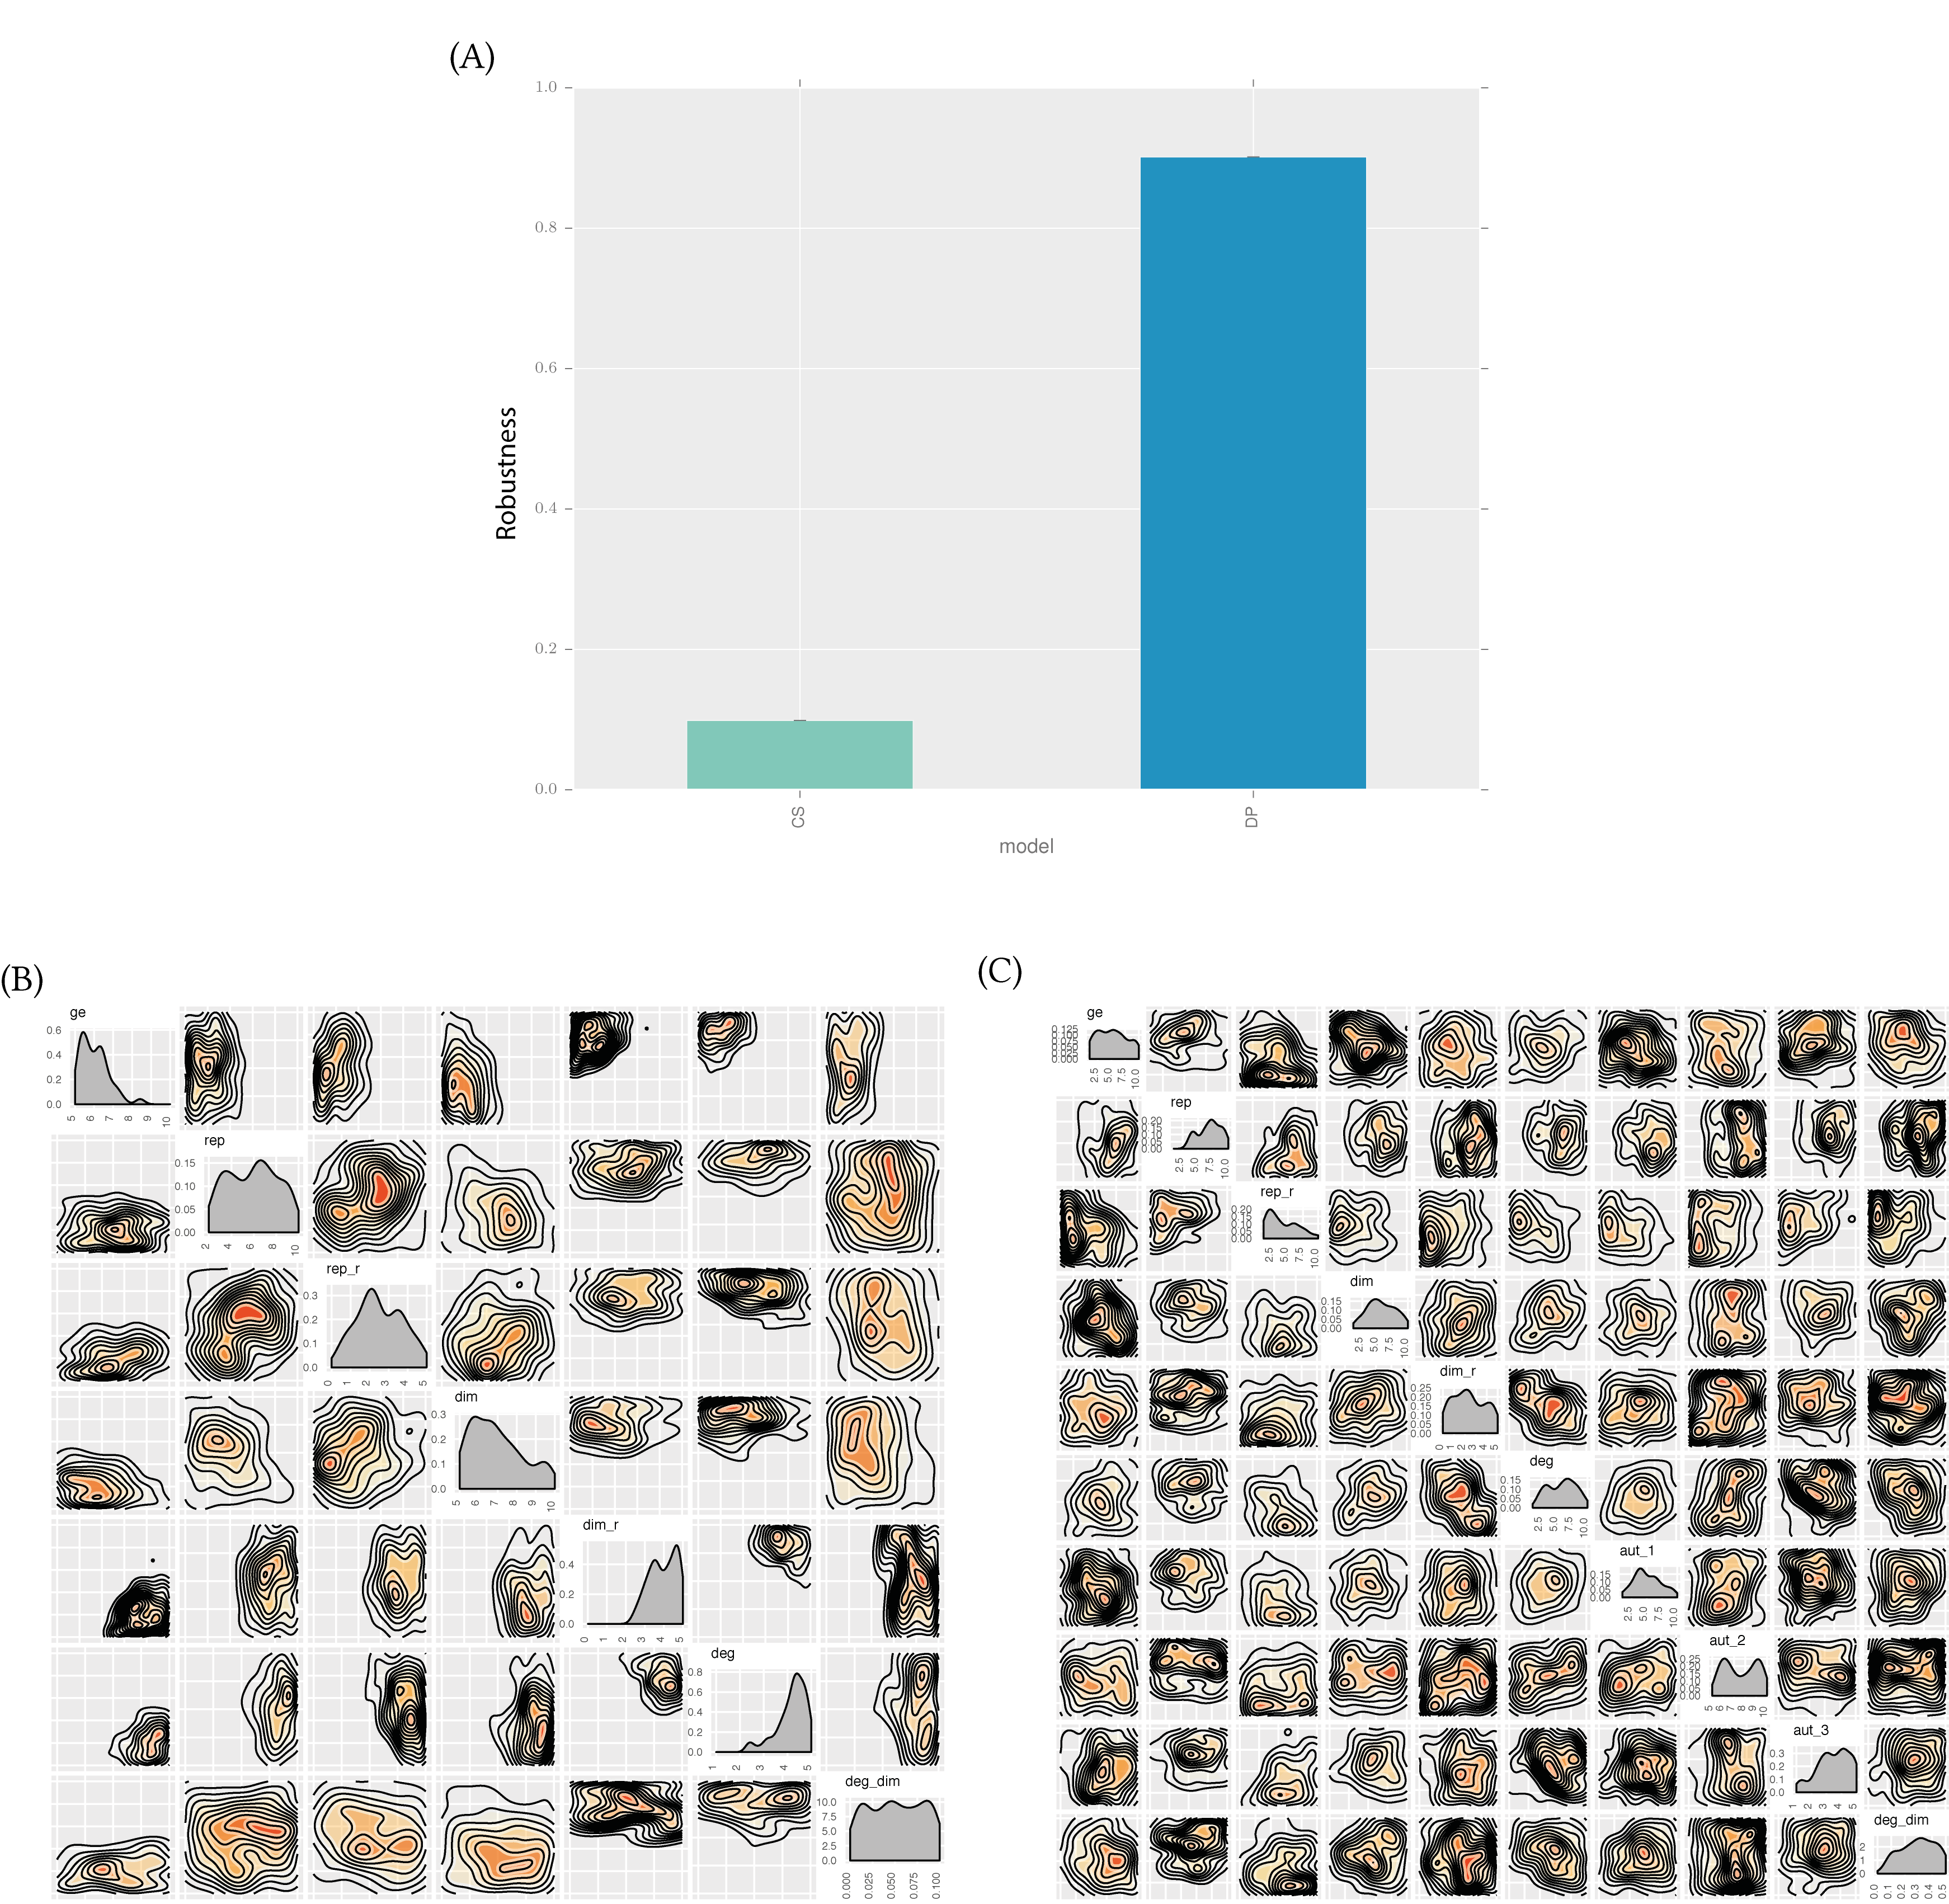
\includegraphics[width=1.1\textwidth]{../../chapters/chapterStabilityFinder/images/MA_sym_post.png}
\caption[Robustness comparison of the \acrshort{cs-ma} and \acrshort{dp-ma} switches]{ \label{fig:ma-sym-det-post}: The posterior distributions of the symmetric deterministic (A) Robustness comparison of the two models. The Bayes factor of $\frac{p(B|CS)}{p(B|DP)}$ was found to be 9.14. (B) \acrshort{cs-ma} and  (C) \acrshort{dp-ma} switches. }
\end{figure*}


By examining the posterior distributions shown in Figure~\ref{fig:ma-sym-det-post} we see that the \acrshort{cs-ma} is much more constrained that the \acrshort{dp-ma} switch. We find that gene expression must be low for bistability to occur in the \acrshort{cs-ma} model but there is no such constraint in the \acrshort{dp-ma} model. We also find that the monomerization rate $dim\_r$ and the monomer degradation rate $deg$ must both be larger than 2. This is not found in the \acrshort{dp-ma} model. 

Next I compare the two models for robustness using the ellipsoid method described in Section~\ref{sec:cal_rob}. We find that the addition of positive feedback loops greatly increases the system's robustness to parameter fluctuations as seen in Figure~\ref{fig:ma-sym-det-post}A, The Bayes factor of $\frac{p(B|CS)}{p(B|DP)}$, where $B$ is bistable behaviour, was found to be 9.14.. Adding positive feedback loops to the model allows it to be bistable over a greater range of parameter values. This indicates that small fluctuations in parameters in the cellular environment will not revert it to monostability and thus makes it more suitable for use in synthetic biological applications where inconsistent stability profile of a system could be detrimental. This makes it a better candidate for building new synthetic devices based on the toggle switch design. We identified the parameter region within which these models are bistable, information that is important when building such a device in the lab.

The models used in the above analysis assume the parameters for equivalent reactions are equal. This is a constraint that simplifies the model. When building this model into a synthetic system in the lab, this assumption is not necessarily justified. When choosing promoters to build this synthetic system two promoters can be chosen to have similar strength but their strength will not necessarily be identical.  In order to study how this might affect the results, I further eliminate modelling assumptions made in the toggle switch by making the parameters representing gene expression ($ge$) and repression ($rep$), as well as the protein degradation parameters asymmetric (independent parameters for each protein, versus fixed to be equal). We find that the features of the posterior distributions of the symmetric and the asymmetric models remain the same. The reader is referred to Appendix~\ref{ap:figures} for the posterior distributions of the asymmetric models. 

%The posterior distribution of the asymmetric \acrshort{cs-ma} model was more constrained than the posterior distribution of the asymmetric \acrshort{dp-ma} model. 

I further study the asymmetric mass action models by examining the \acrshort{qssa}. As stated in Section~\ref{sec:qssa}, the \acrshort{qssa} is a common analytical tool for model simplification. By examining the posterior distributions of the \acrshort{cs-ma} we can determine whether the \acrshort{qssa} is justified in these models. As stated in Section~\ref{sec:qssa}, the assumption that has to be made for the \acrshort{qssa} to hold is that the rate of binding and unbinding of the transcription factors to the promoters is very fast. The rates have to be much faster than the rates of their production and decay in the system in order to justify that the reaction take place in separate time scales and can thus be assumed to always be at steady state. The \acrshort{qssa} is also made for the dimerization of the transcription factors. Therefore, for the \acrshort{qssa} to be justified in the toggle switch, the rates for association ($rep$) and dissociation ($rep\_r$) of the transcription factors to the promoters, as well as the rates for dimerization ($dim$) and monomerization ($dim\_r$) of the transcription factors have to be much larger than any other rate.


In order to determine whether this is the case here, I plot the marginal distributions of each of the parameters assumed to be very large ($rep$, $rep\_r$, $dim$, $dim\_r$) against each of the parameters involved in the expression and decay of the proteins. This is shown in Figure~\ref{fig:ma_qssa}. We find that the \acrshort{qssa} can be justified only with respect to the rate of degradation of the transcription factor dimers ($deg\_dim$). All parameters under consideration for the \acrshort{qssa} ($rep$, $rep\_r$, $dim$, $dim\_r$) are found to be much larger than $deg\_dim$. On the other hand, the \acrshort{qssa} cannot be justified with respect to gene expression ($ge$) or protein degradation ($deg$). It is seen in Figure~\ref{fig:ma_qssa} that the rates under consideration for the \acrshort{qssa} are not much larger than the rates of protein production and decay, and thus it cannot be assumed that they are always at steasdy state. This means that the CS-MA model functions as a switch even when the \acrshort{qssa} does not hold. These assumptions, necessary for the reduction of the model, are therefore not always justified in this case. 

% If $rep$, $rep_r$, $dim$ and $dim_r$ are much larger than the rates for production and decay of the proteins, the distribution will be  




\begin{figure*}[htbp]
\begin{center}
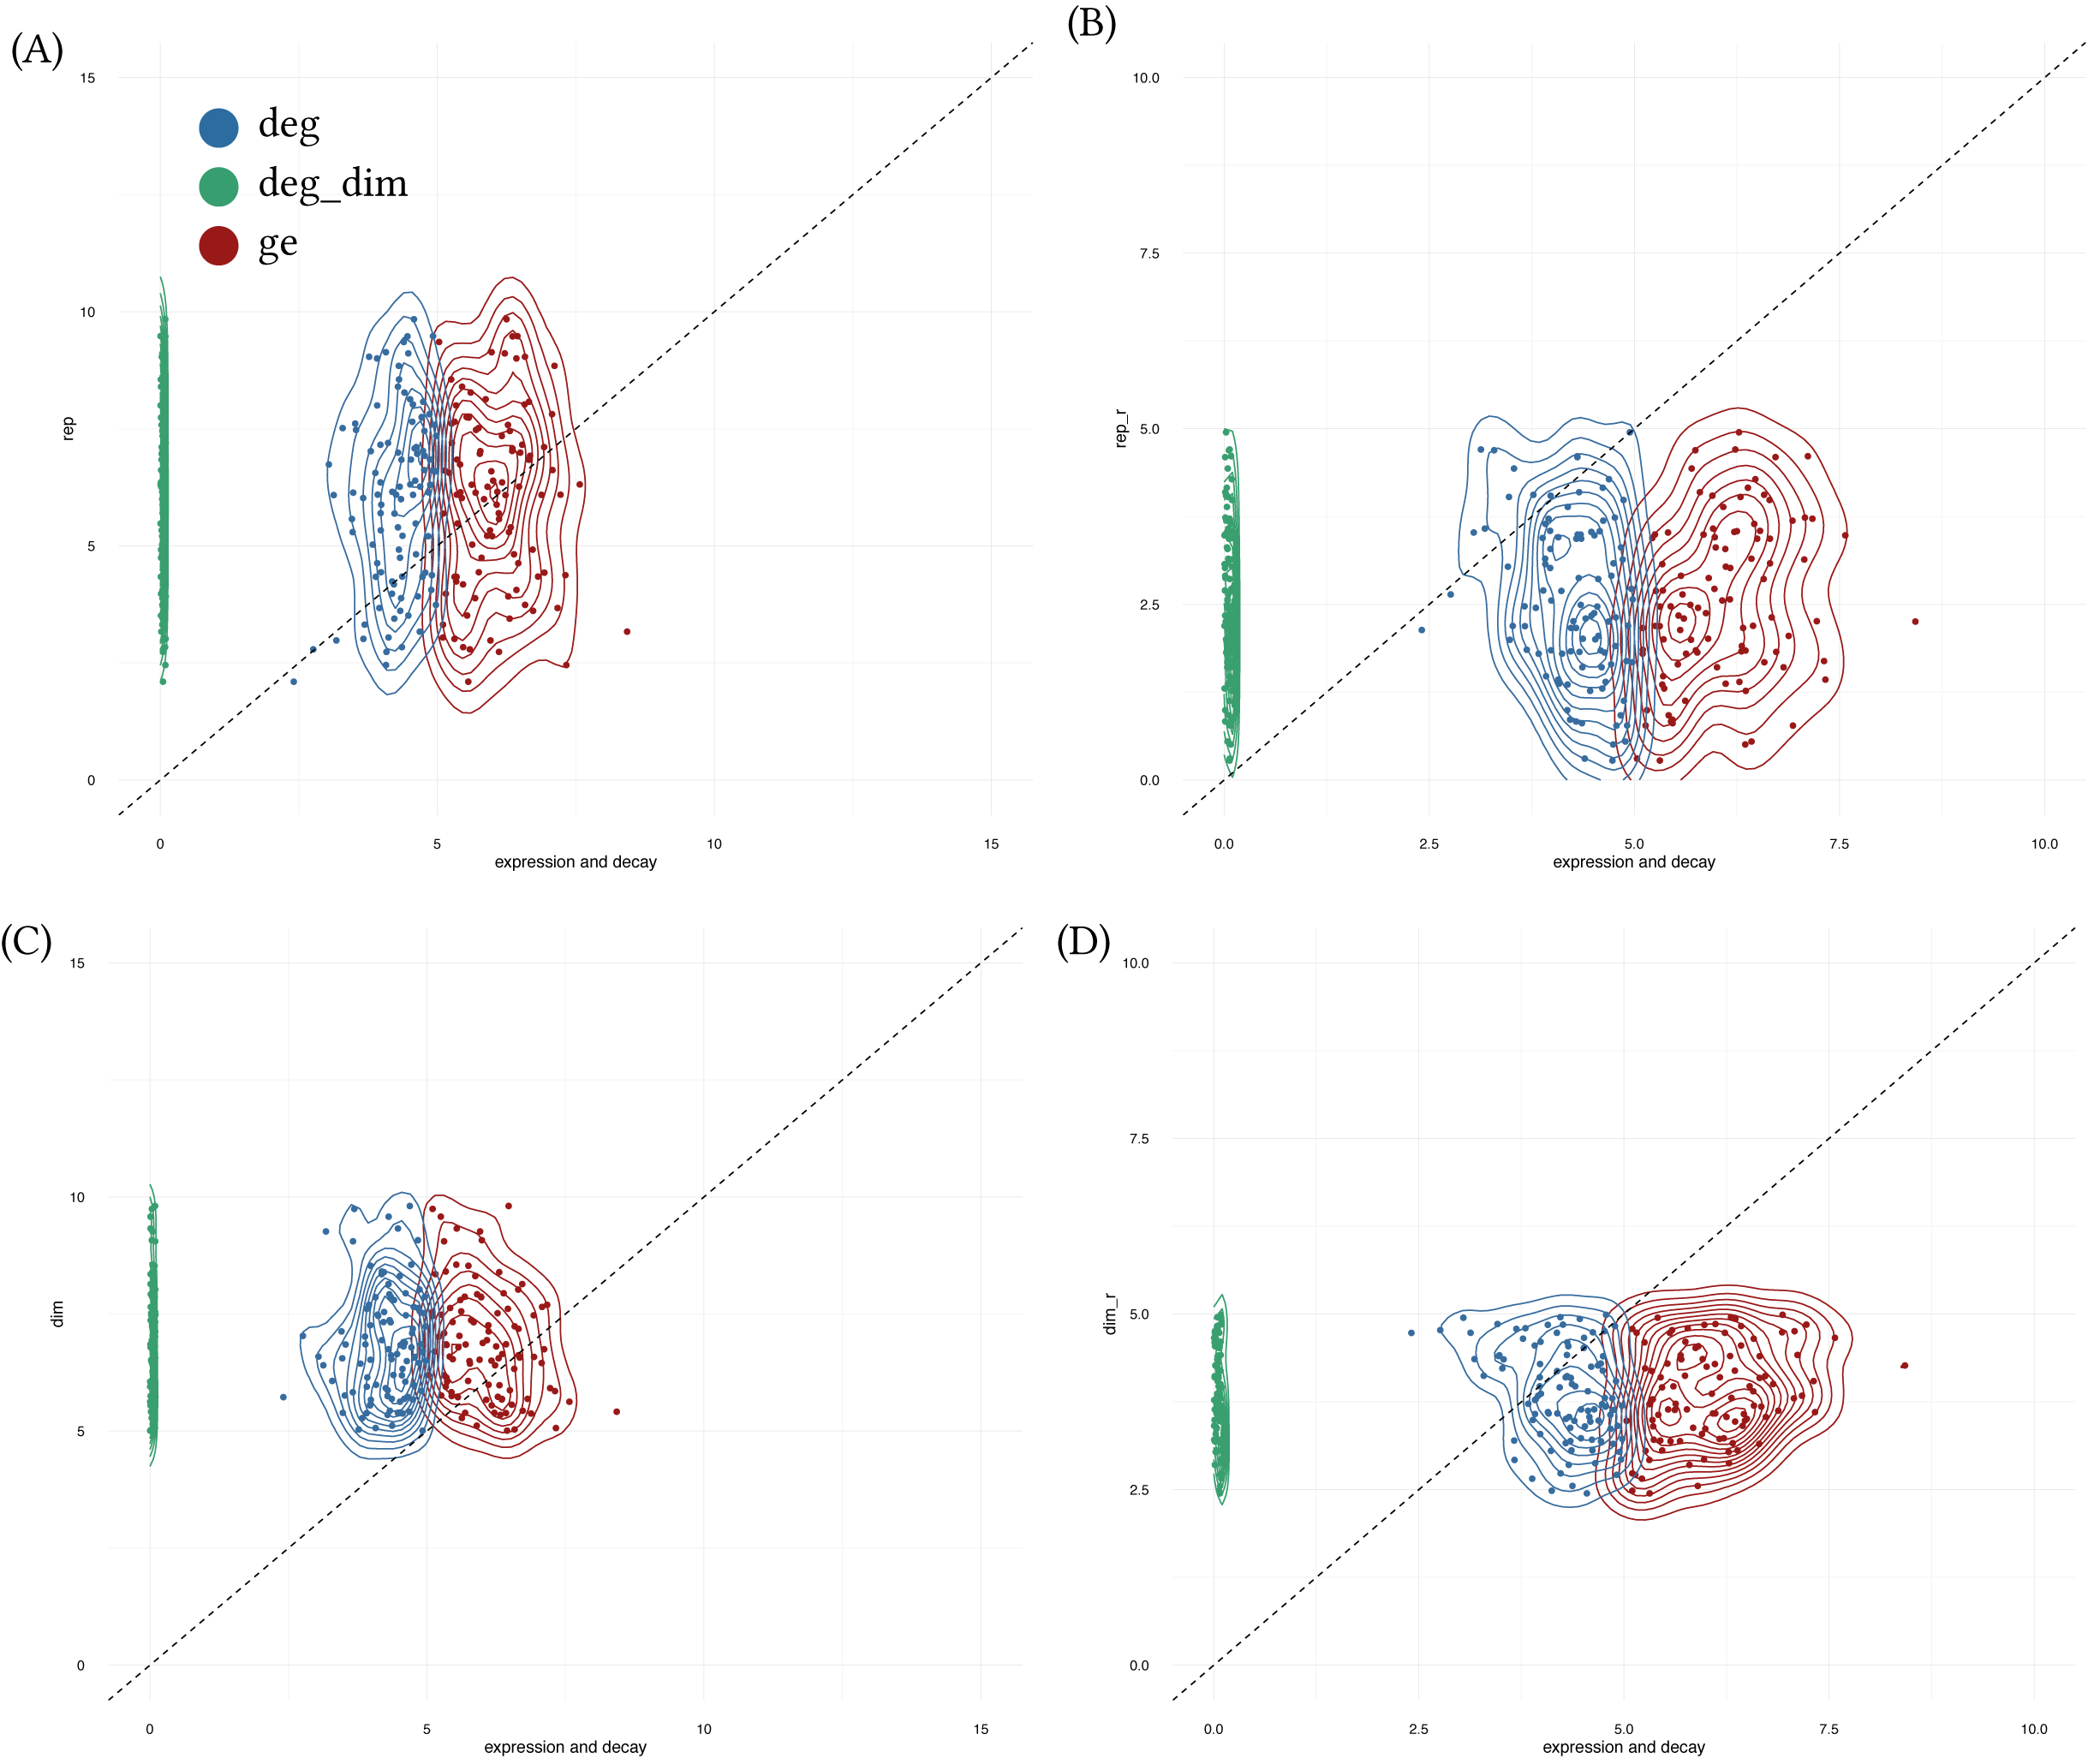
\includegraphics[width=\textwidth]{../../chapters/chapterStabilityFinder/images/qssa-cs-sym.png}
\caption[Testing the QSSA assumptions on the mass action models]{ \label{fig:ma_qssa}: The \acrshort{qssa} cannot be justified for the CS-MA model. The dotted line denotes the line where $x = y$. The posterior distributions of the rates under consideration, $rep$, $rep\_r$, $dim$, $dim\_r$, are all much larger than the rate of degradation of the transcription factor dimer. (A) The rate of binding of the repressors to the promoter is not much larger than the rate of protein expression and degradation. (B) The rate of protein expression and decay are both larger than the rate of dissociation of the dimer to the promoter. (C) The rate of transcription factor dimerization is larger than the rates of protein production and decay, but not by a big amount. (D) The rate of monomerization of the transcription factors is smaller than the rates of protein expression and decay.}
\end{center}
\end{figure*}
\clearpage


%I further investigated modelling assumptions by separating transcription and translation into two separate steps. This makes the models more realistic but also more complex and StabilityFinder is ideal for analysing them.  It is known that transcription in prokaryotes occurs in bursts~\cite{Golding:2005uv} so an interesting question is whether transcriptional bursting has an effect on bistability. To investigate this I added a multiplicative term to the \acrshort{ode}s for mRNA production. Using StabilityFinder on these models we find that transcriptional bursting does not affect a system's ability to be bistable. 

\subsubsection{Multistability in the stochastic mass action switches}

To investigate how the level of abstraction affects switch design principles, I expand the analysis under the assumption of mass action kinetics and stochastic dynamics. The asymmetric \acrshort{cs-ma} and \acrshort{dp-ma} models are simulated using the Gillespie algorithm~\autocite{Gillespie:1977ww}.

\textcite{Ma:2012dt} found that the stochastic fluctuations in a system involving such a small number of molecules, like the toggle switch, uncovers effects that can not be predicted by the fully deterministic case~\autocite{Ma:2012dt}. We find that in the stochastic case, both the simple switch, \acrshort{cs-ma} , and positive autoregulation switch, \acrshort{dp-ma}, are capable of both bistable and tristable behaviour. The fact that tristability can occur in the classical model is consistent with the effect of small molecule numbers; if gene expression remains low, it provides the opportunity for small number effects to be observed, and the third steady state to stabilise \autocite{Ma:2012dt}. In order to ensure that the tristable switches found in the stochastic case are truly tristable, I re-sample the posterior distributions and simulate to steady state. If the resulting phase plots are tristable then we know that the posterior truly represents tristability. 


\begin{table}[tb]
\centering
\caption{Design principles of the stochastic MA bistable and tristable switches}
\label{tab:des_prin}
\begin{tabular}{@{}ccccc@{}}
\toprule
                    & \multicolumn{2}{c}{\textbf{\acrshort{cs-ma}}} & \multicolumn{2}{c}{\textbf{\acrshort{dp-ma}}} \\ \cmidrule(l){2-3}\cmidrule(l){4-5}
                    & \textit{Bistable}    & \textit{Tristable}   & \textit{Bistable}    & \textit{Tristable}   \\\cmidrule(l){2-2}\cmidrule(l){3-3}\cmidrule(l){4-4}\cmidrule(l){5-5}
dimerisation        & High        & Low         & High        & Low         \\
protein degradation & -           & -           & -           & Low         \\
dimer degradation   & Low         & -           & Low         & -           \\\bottomrule
\end{tabular}
\end{table}

As can be seen in Figure~\ref{fig:fig7}, differences in the parameter values are observed between the bistable and tristable switches, in both\acrshort{cs-ma} and \acrshort{dp-ma} models. We find that the simple switch is tristable when dimerisation rate is low and bistable when it is high. The degradation of the dimer proteins must have a low rate for bistability but there are no restraints in the case of the tristable switch. For the case of the DP switch, we find that the rates for dimerisation, degradation and dimer degradation are different for the bistable and tristable behaviours (Figure~\ref{fig:fig7}). The rate of dimerisation must be low for tristability to occur and large for bistability, as observed for the simple switch. The parameter for protein degradation must be low for tristability whereas there are no constraints for the bistable case. Finally, the parameter for dimer degradation must be low for bistability whereas it has no constraints for tristability, as observed in the simple switch. The design principles for both the \acrshort{cs-ma} model and the \acrshort{dp-ma} model are summarised in Table~\ref{tab:des_prin}



\begin{figure*}[htbp]
\centerfloat
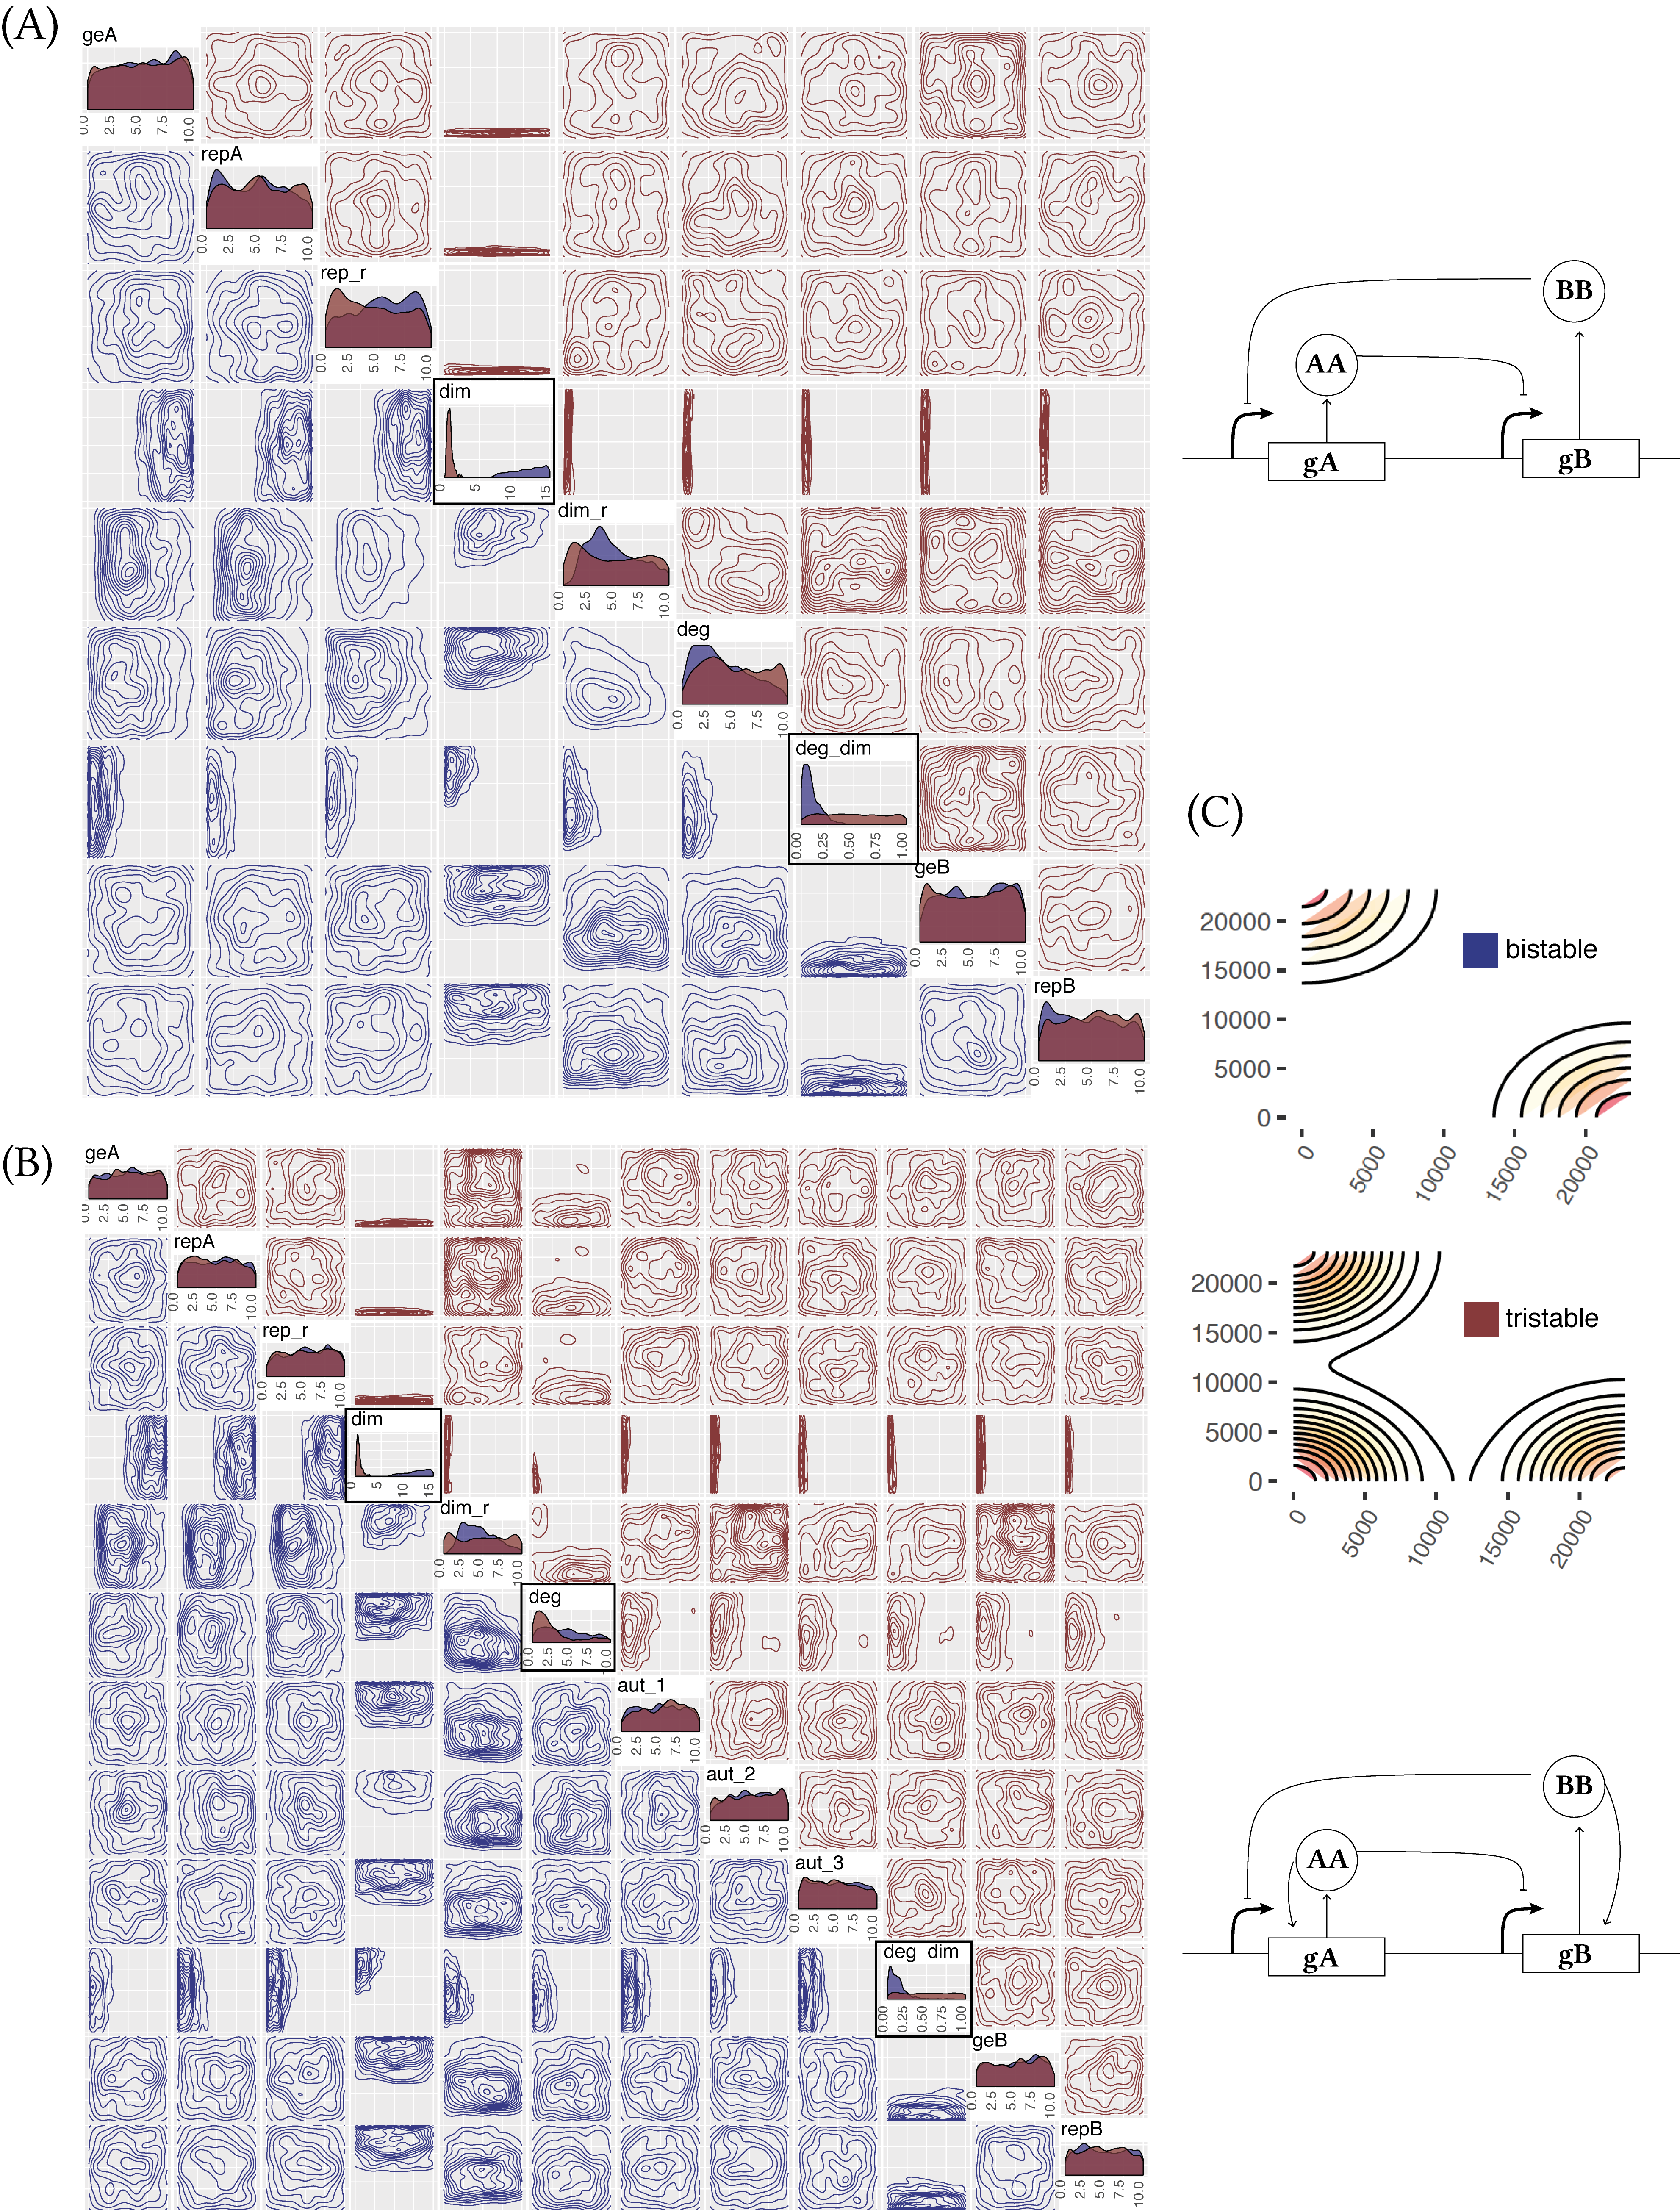
\includegraphics[width=1.1\textwidth]{../../chapters/chapterStabilityFinder/images/MA_stoch_design_princ.png}
\caption[Multistability in the stochastic mass action models]{ \label{fig:fig7}: Tristability is possible in the mass action toggle switch models only when simulated stochastically. (A) The simple toggle switch with no autoregulation can be both bistable and tristable. The two posteriors are shown, where the posterior distribution of the bistable switch is shown in red and of the tristable switch in blue. From the posterior distribution we can deduce the the dimerization parameter must be small for tristability to occur but large for bistability. The switch with double positive autoregulation and its posterior distributions for the bistable and tristable case are shown in (B). (C) A sample phase plot of a stochastic tristable and bistable mass action switch. }
\end{figure*}
\clearpage


\subsubsection{Bayes factors depend on the choice of priors}

An important aspect of Bayes factors, and thus robustness, that must be investigated is its dependence on the prior distributions. From Equation~\ref{eq:final_bayes} we can expect that the measure for robustness will depend on the size of the prior. The prior distributions for model comparison are ideally chosen by using related data that can inform the choice. But this situation can be rare and priors are selected by using information from the literature in combination with rough guesses~\autocite{Kass:1995eh}. Often simplifications are made and the choice of large prior ranges can seem like like an attractive option, as to impose less bias to the priors. Nevertheless this can have an effect on the Bayes factors calculated. The choice of improper, or very large priors can skew Equation~\ref{eq:final_bayes} to favour one model over the other~\autocite{Kass:1995eh}. In this section I demonstrate that the choice of priors for the toggle switch models has a significant effect on the calculated robustness of the models. This has to be taken under consideration when analysing candidate models for use in synthetic biology applications, as a poor choice of priors can skew the robustness analysis in favour of one model over the other, when no such robustness gain will be observed \textit{in vivo}.    

In order to demonstrate the effect of prior choice on robustness, I use the \acrshort{cs-ma} model. I use StabilityFinder to approximate the posterior distribution that makes this model bistable using two ranges of prior distributions. The two sets of prior distributions used here are denoted as very narrow (VN2) and wide (W) in Table~\ref{tab:prior_study}. The posterior distributions obtained corresponding to the VN priors and W priors are shown in Figure~\ref{fig:priors_matter}A and B respectively. It can be seen that the posterior distribution of the model with VN2 priors is more constrained that the model with W priors. This indicates that if one of the parameters is able to have a larger value, then the constraints on the rest of the parameters are not necessary any more. This results in the unconstrained posterior distribution observed in Figure~\ref{fig:priors_matter}B.

\begin{table}[tb]
\centering
\caption{Priors used for studying the effect of priors to robustness}
\label{tab:prior_study}
\begin{tabular}{@{}cccc@{}}
\toprule
         & VN2 & N1  & W    \\ \midrule
ge       & 5 - 10      & 1 - 10  & 1 - 100 \\
rep      & 2 - 10      & 1 - 10  & 1 - 100 \\
rep\_r   & 0 - 5       & 1 - 10  & 0 - 10  \\
dim      & 5 - 10      & 1 - 10  & 0 - 10  \\
dim\_r   & 0 - 5       & 0 - 5   & 0 - 10  \\
deg      & 1 - 5       & 0 - 10  & 0 - 100 \\
deg\_dim & 0 - 0.1     & 0 - 0.5 & 0 - 1   \\ \bottomrule
\end{tabular}
\end{table}

Furthermore, I test the effect of the prior range to the robustness of the model for each parameter separately. For each test, the prior distributions of all the parameters correspond to the range given in column VN2 in Table~\ref{tab:prior_study} except for the parameter being tested. For each run one parameter is being tested and has a prior range equal to the range given in column W in Table~\ref{tab:prior_study}. StabilityFinder is then used to approximate the posterior distribution of the model, given the priors and bistable behaviour. Therefore, there are 7 posterior distributions of the bistable CS-MA switch, each one corresponding to one parameter having a wide prior range. For each run, the Bayes factor of the model compared to the \acrshort{dp-ma} model used in Figure~\ref{fig:ma-sym-det-post} is calculated, using Algorithm~\ref{alg:robustness}. The posterior distribution for \acrshort{dp-ma} remains the same every time. Figure~\ref{fig:priors_matter}C shows the Bayes factors calculated for the DP-MA model against each run of the \acrshort{cs-ma}. We can see from Figure~\ref{fig:priors_matter}C that when the priors for $ge$ are much larger, the Bayes factor increases. The evidence for choosing DP-MA over CS-MA changes from substantial to strong, as defined in Table~\ref{tab:BAYES_FACTS}, by using a larger prior for parameter $ge$. This change is attributed to the fact the $ge$ is constrained to be low. If the prior range is much larger, it is evident that the ratio of the volumes of the functional region to the prior will be much smaller for CS-MA. %On the other hand, the range of the prior of parameter $deg\_dim$ does not increase the Bayes factor in favour of model DP-MA. This is in agreement with~\textcite{Kass:1995eh}, who 
 

\begin{figure*}[h]
\begin{center}
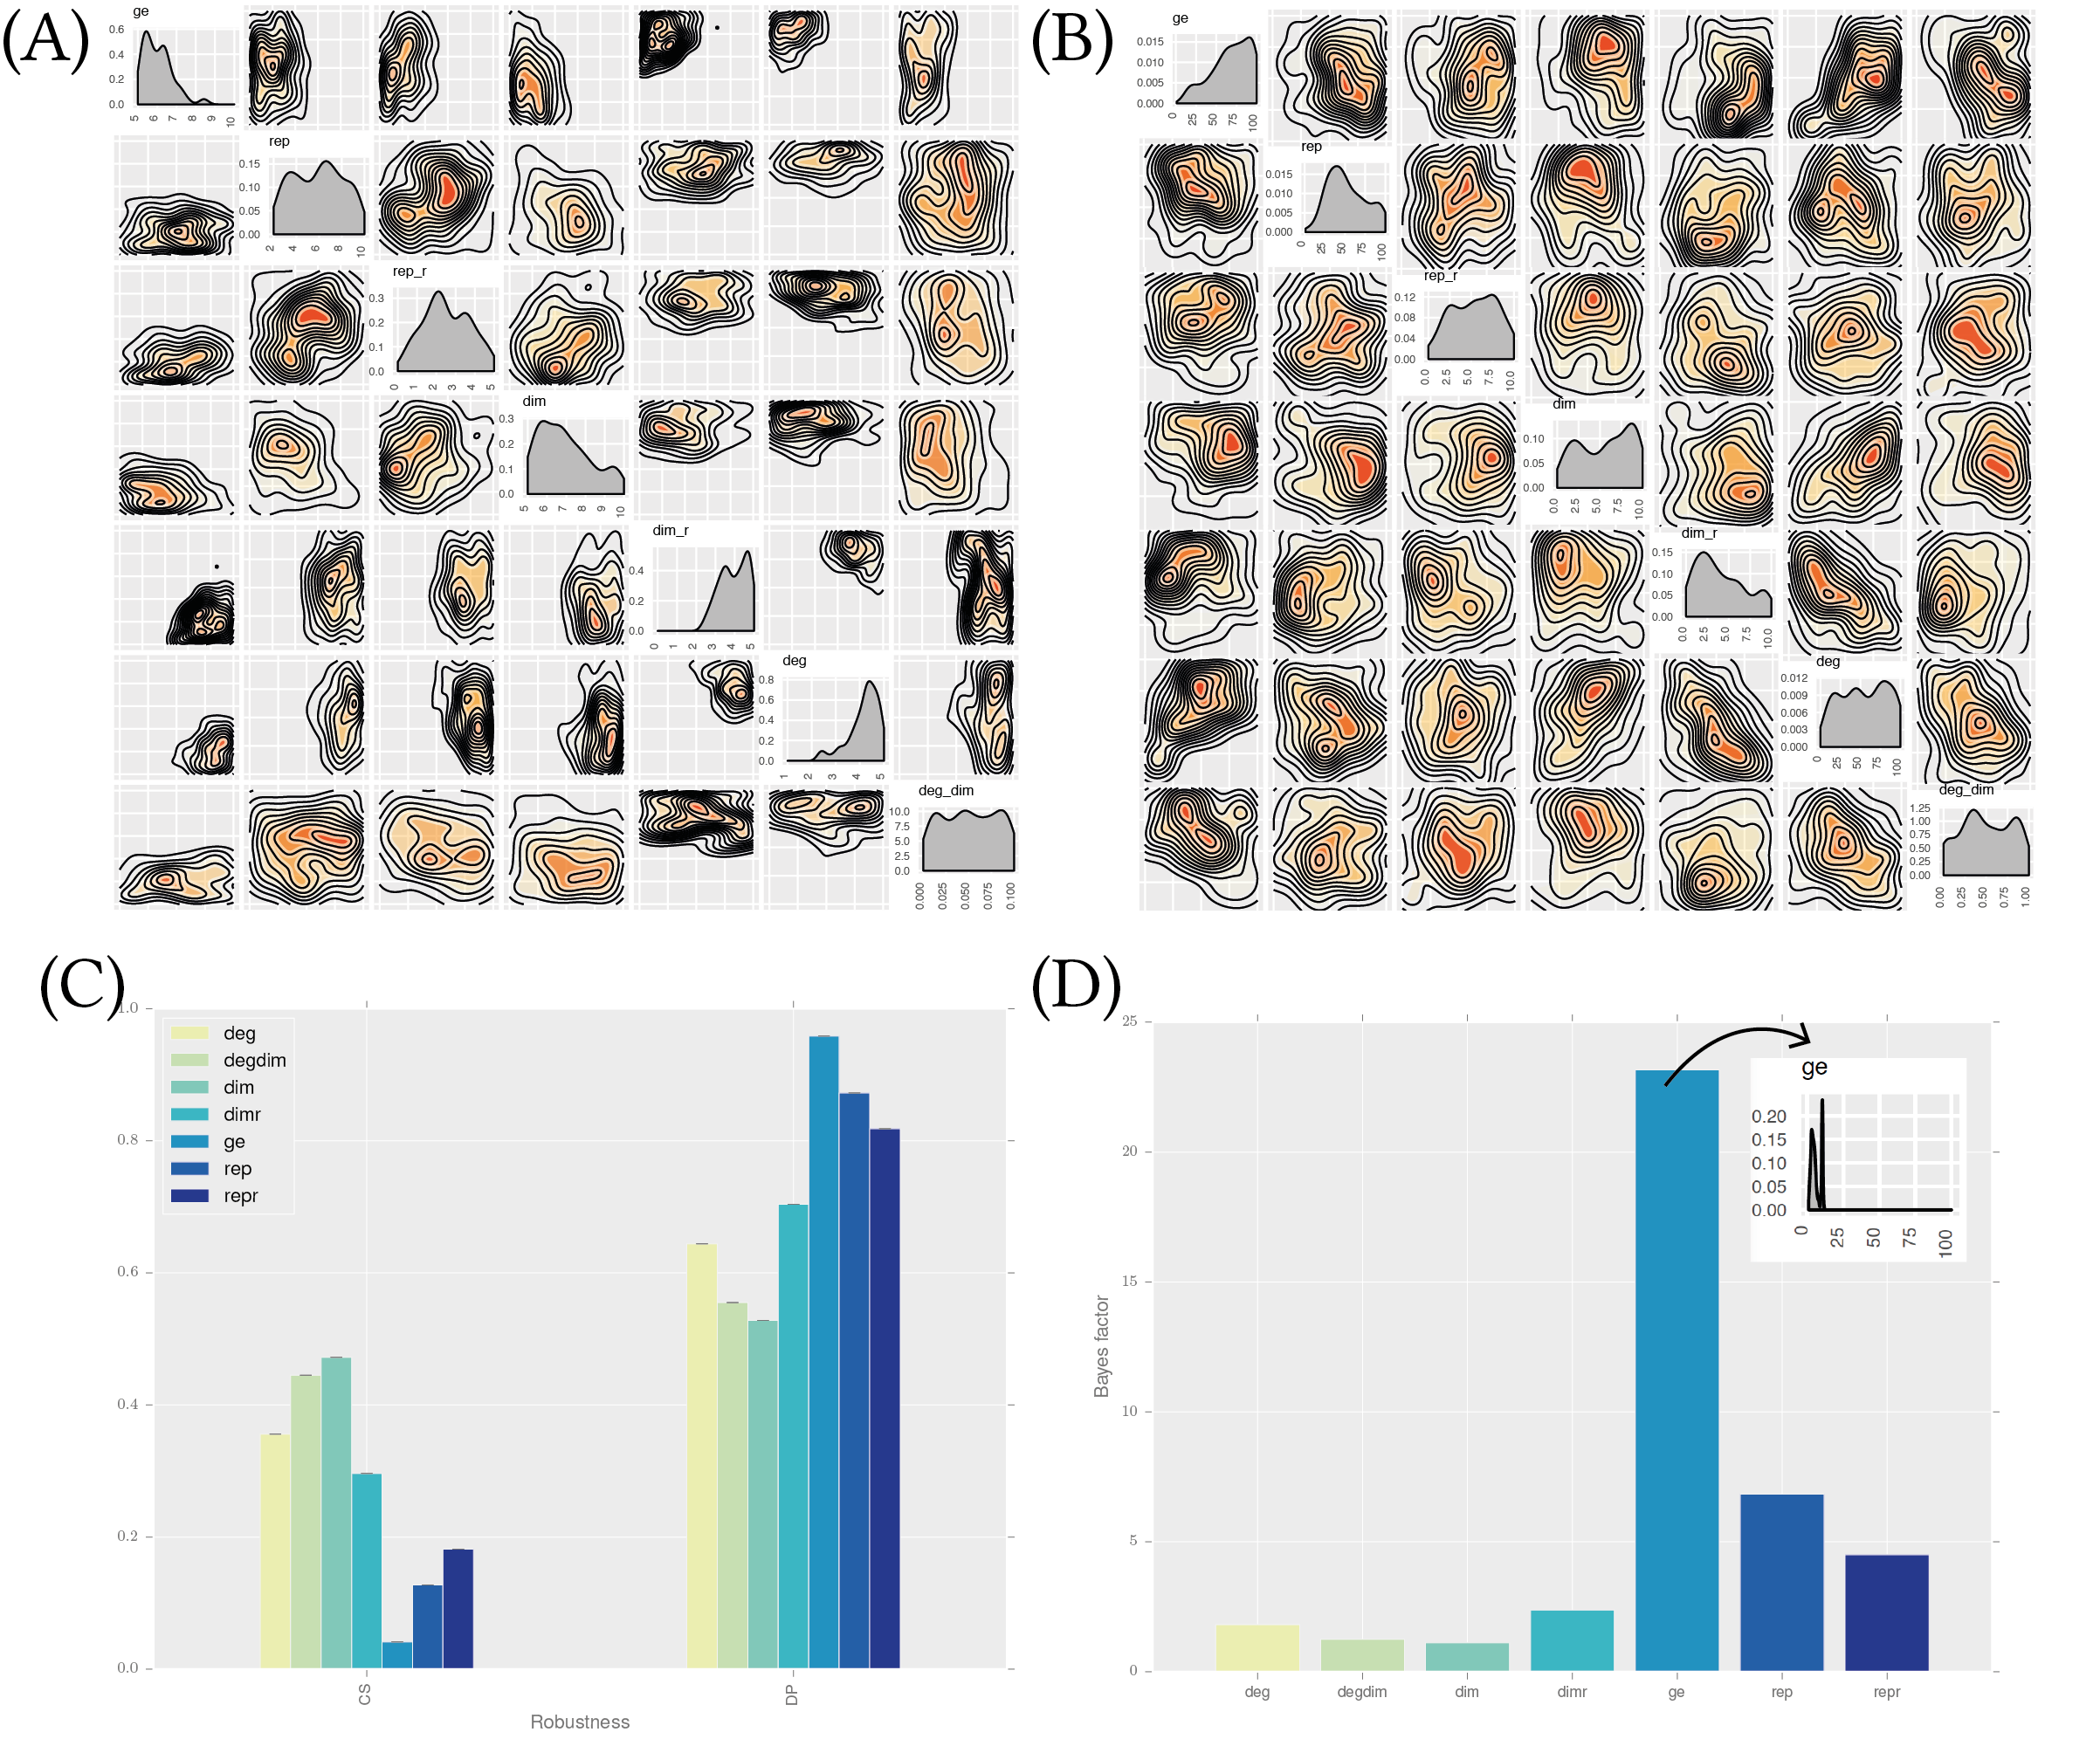
\includegraphics[width=1.2\textwidth]{../../chapters/chapterStabilityFinder/images/priors_matter.png}
\caption[The volume of the priors has an effect on the posterior distribution obtained.]{ \label{fig:priors_matter}: The volume of the priors has an effect on the posterior distribution obtained. (A) The \acrshort{cs-ma} model with VN2 priors and (B) the \acrshort{cs-ma} with W priors. (C) The increase in robustness seen is due to the gene expression parameter prior being wide while the functional region remains constrained.}
\end{center}
\end{figure*}



In Section~\ref{sec:ma_sw} we found that the \acrshort{dp-ma} is more robust than the \acrshort{cs-ma} model. Here I want to test whether this result still remains when the priors of the models are made wider. In order to test that, I change the prior ranges of both models and measure their robustness each time using Algorithm~\ref{alg:robustness}. The classes of priors used are given in Table~\ref{tab:prior_study}. The robustness measures calculated, which corresponds to the fraction of the volume of the functional region over the volume of the prior, are shown in Figure~\ref{fig:priors_matter2}A. 

%The Bayes factors, corresponding to the ratio of the robustness measure of \acrshort{dp-ma} to the robustness measure of \acrshort{cs-ma} is given relative to the difference in the volumes of the priors of the two models in Figure~\ref{fig:priors_matter2}B.

We find that the robustness measure changed as the priors of the models changed. When both models have very narrow or when both models have wide priors then their robustness measures are very similar. When both models have vary narrow priors the Bayes factor is equal to 1.32 and when the priors are wide the Bayes factor is equal to 1.06. In both these cases the Bayes factor is less than 3.2, and therefore is considered not significant~\autocite{Kass:1995eh}. When the priors for both models are narrow, the Bayes factor is equal to 2.25, which is still considered not significant. Most notably, when the priors for the \acrshort{cs-ma} model are very narrow and the priors of the \acrshort{dp-ma} model are narrow, the Bayes' factor is at 9.14. The Bayes factor is now greater than 3.2, but less than 10, and is thus considered substantial~\autocite{Kass:1995eh}.  These results are summarised in Table~\ref{tab:bayes_vols}.

\begin{table}[tb]
\centering
\caption{Bayes factors of the \acrshort{dp-ma} against the \acrshort{cs-ma}  model using different volumes of priors}
\label{tab:bayes_vols}
\begin{tabular}{@{}ccc@{}}
\toprule
\multicolumn{2}{l}{Prior volume} & \multirow{2}{4cm}{Bayes factor  ($\frac{p(B|DP-MA}{p(B|CS-MA)}$)  } \\ \cmidrule(r){1-2}
\acrshort{cs-ma}  & \acrshort{dp-ma} &  \\ \midrule
VN2 & VN2 & 1.32 \\
VN2 & N1 & 9.14 \\
N1 & N1 & 2.25 \\
W & W & 1.06 \\ \bottomrule
\end{tabular}
\end{table}

It is evident that the robustness measure depends on the prior volume. It is therefore useful to think of the Bayes factor in terms of the difference in the volume of the priors of the models that are being compared. I carry out this analysis for the above priors and the results are shown in Figure~\ref{fig:priors_matter2}B. Here we see that even though the prior difference is within the same order of magnitude, the Bayes factor increases significantly. This point corresponds to the case where the priors of \acrshort{cs-ma} are very narrow and the priors of \acrshort{dp-ma} are narrow, and that is where we see the Bayes factor between the two models maximise. %We can take advantage of this observation to design a switch with double positive autoregulation that is significantly more robust than the Gardner toggle switch. By choosing the parameter values carefully we can maximise the gain of robustness that adding two positive feedback loops gives. 

\begin{figure*}[h]
\begin{center}
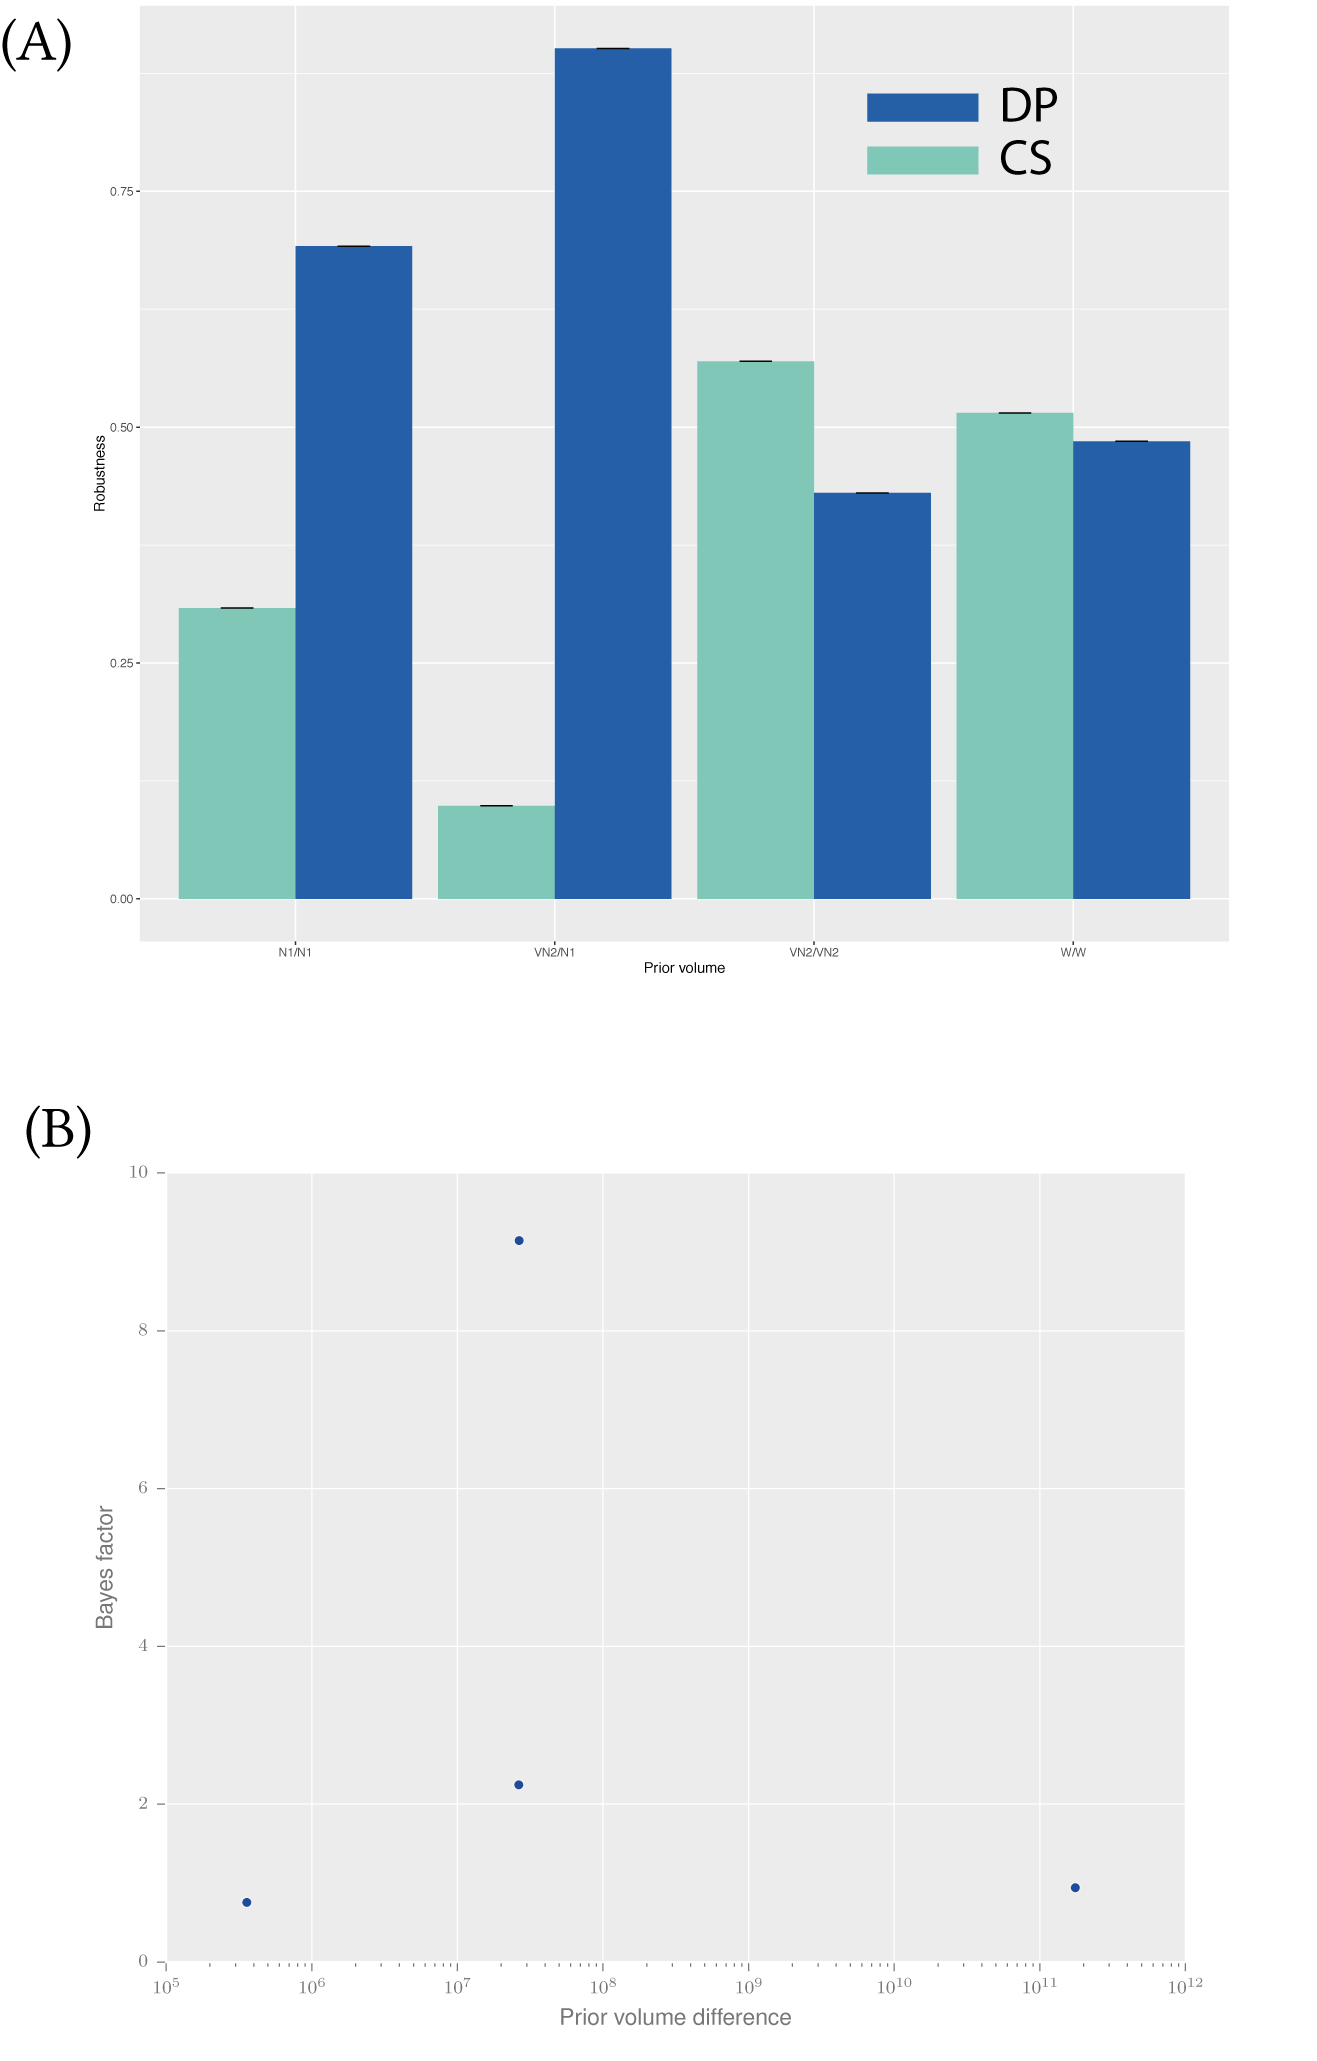
\includegraphics[scale=0.7]{../../chapters/chapterStabilityFinder/images/priors_matter_2.png}
\caption[Changing the priors in both models affects the robustness measure.]{ \label{fig:priors_matter2}: Changing the priors in both models affects the robustness measure. (A) Using different prior ranges for the \acrshort{cs-ma} and the \acrshort{dp-ma} models yields different robustness for each. (B) The Bayes factor as a function of the prior volume difference. }
\end{center}
\end{figure*}

These results highlight the importance of choosing the ranges of priors for the models under consideration carefully. A balance has to be struck between restricting the prior ranges too much, where interesting behaviour in the model can be missed, and making the prior range too wide, where it becomes uninformative. 

\clearpage
%This indicates that small fluctuations in parameters in the cellular environment will not affect the system's ability to be bistable, and thus makes it more suitable for use in synthetic biological applications where a very constrained parameter set can be too restrictive.% This makes it a better candidate for building new synthetic devices based on the toggle switch design.

%We identified the parameter region within which these models are bistable, information that is important when building such a device in the lab. In the future, by selecting the system components accordingly, the parameter values can be adjusted \textit{in vivo}. For example, the desired level of gene expression can be accomplished by selecting the appropriate RBS sequence~\autocite{Salis:2009gk}. Another method to modify the parameter values \textit{in vivo} is to select the promoter to have the strength corresponding to the levels of gene expression and repression desired. Activity of each promoter can be measured and standardised~\autocite{Kelly:2009bj} making this process possible. For a system requiring more than one promoter, these can be efficiently selected from a promoter library using a genetic algorithm~\autocite{Wu:2011bq}. These standardised interchangeable components with known sequence and activity~\autocite{Kelly:2009bj,Canton:2008fv} can be selected and used to construct a desired system and replicate the parameter values found using StabilityFinder.

\section{Discussion}
  
 %This is critical to the design of novel synthetic switches, where the stability of a system has to be well defined and predictable.
 
 Here I developed a novel framework, StabilityFinder, that can be used to infer parameter values that can produce a desired behaviour. The novelty in the framework I developed over existing methodology is that complex models can be analyzed assuming either deterministic or stochastic dynamics. I have used StabilityFinder to uncover the design principles of a bistable, a tristable and a quadristable switch. I found key parameters that are important in determining the number of steady states a system is capable of. This is important to the design of novel synthetic switches, where the genetic parts chosen, with their corresponding reaction rates can have an effect on the stability of the system. A bistable, a tristable or a quadristable switch could each be used for different functions within a synthetic system. 
  
   %This is especially true when multiple such systems are used together, and the success of the whole system depends on all the parts working as expected. 
   
Being able to \textit{in silico} determine the stability a given system will aid in the design of novel synthetic circuits. In the future, by selecting the system components accordingly during sequence design, the parameter values can be selected \textit{in vivo}. For example, the parameter value corresponding to the translation initiation rate can be chosen by selecting the appropriate RBS sequence which given a nucleotide sequence will produce the desired rate~\autocite{Holtz:2010bm}, a method developed by~\textcite{Salis:2009gk}. Another method to tweak the parameter values \textit{in vivo} is to select the promoter to have the strength corresponding to the levels of gene expression and repression desired. Activity of each promoter can be measured and standardised~\autocite{Kelly:2009bj} making this process possible. For a system requiring more than one promoter, these can be efficiently selected from a promoter library using a genetic algorithm created by~\textcite{Wu:2011bq}. These standardised interchangeable components with known sequence and activity are what synthetic biology classes as BioBricks~\autocite{Kelly:2009bj,Canton:2008fv} and can be selected and used to construct a desired system.

 Nevertheless, it is important to note that StabilityFinder predicts the stability of a system in isolation. Recent body of work has shown that modules like the one studied here are not independent of downstream processes~\autocite{DelVecchio:2008gy, Ventura:2010ew, Jiang:2011ch, Lyons:2014iq}.~\textcite{Lyons:2014iq} showed that adding a downstream load to the genetic toggle switch can render it monostable. In order for multi-module systems to be successful, the effect of downstream loads to the system under study will have to be considered. Therefore extrapolation of the conclusions of StabilityFinder for a given module would not be justified when the module is part of a larger system of modules working in tandem.        
    
 %THIS IS ALL WORD FOR WORD FROM BACKGROUND OF CHAPTER ABC-SYSBIO CHANGE ONE OF THEM ASAP
% Tools that can identify parameter regions that give rise to specific behaviours will be key for the success of synthetic biology. In the future, by selecting the system components accordingly, the parameter values can be adjusted \textit{in vivo}. For example, the desired level of gene expression can be accomplished by selecting the appropriate RBS sequence~\autocite{Salis:2009gk}. Another method to modify the parameter values \textit{in vivo} is to select the promoter to have the strength corresponding to the levels of gene expression and repression desired. Activity of each promoter can be measured and standardised~\autocite{Kelly:2009bj} making this process possible. For a system requiring more than one promoter, these can be efficiently selected from a promoter library using a genetic algorithm~\autocite{Wu:2011bq}. These standardised interchangeable components with known sequence and activity~\autocite{Kelly:2009bj,Canton:2008fv} can be selected and used to construct a desired system and replicate the parameter values found using StabilityFinder.

The methodology used here can only be used to study the presence of a given stability and not its absence. If the algorithm is not converging it cannot be concluded that the given model is not capable of the desired stability under these priors. For example, the mass action switches were found to be both bistable and tristable when stochastic effects were taken into account. Using deterministic dynamics the algorithm did not converge using priors within the ranges used in this work. Nevertheless this does not permit the conclusion of absence of tristability in the deterministic classic or double positive mass action switch models. StabilityFinder only permits the interpretation of models that have converged to a given stability. 




StabilityFinder can also be used to study the topology of more complex multistable switches that exist in natural biological systems such as developmental pathways. I also limited this framework to the objective behaviour of a given number of stable steady states. This could be extended to examine systems with a given switching rate or systems robust to a particular set of perturbations, both of which could be of great importance for building more complex genetic circuits.

Importantly I find that the prior distributions used during such an analysis greatly affect the robustness observed. More generally, the assumptions made when building a model can have a significant effect on the predictions made. This is consistent with current understanding~\autocite{Babtie:2014jg} and highlight the importance of a programme of experimental work, combined with systems modelling, in order to understand the rules of thumb for abstraction in model based design of synthetic biological systems.

\section{Summary}

In this chapter I discussed the algorithm I developed and demonstrated how it can identify the parameter regions necessary for a model to achieve a given number of stable steady states. I used it to uncover the underlying principles that govern the stability of a given switch. 

I first tested StabilityFinder on a known switch and then proceeded to apply it to more complex models. I uncovered the design principles that make the Lu switch bistable, tristable or quadristable. I extended the Lu models to a three-node switch and showed how it can achieve 6 steady states. 

Furthermore, I built two novel models of the toggle switch which do not use the \acrshort{qssa} and showed that the \acrshort{qssa} cannot be justified in these models. Using these models I studied the effect positive autoregulation has on the robustness of a model. I also studied the effect the priors have on the posteriors and on the robustness of a model. Finally, using stochastic modelling I showed that these switch models are capable of both bistable and tristable behaviour. 

In the next chapter I study the genetic toggle switch in the lab and fit the toggle switch models used here to experimental data. 




